\documentclass[a4paper, usecolor, twoside, onehalfspacing, 11pt]{bwthesis}
% The usecolor option sets the titles in blue, as requested by
% the Ghent University housestyle. Remove this to get a black
% and white version of things.
\usepackage[dutch]{babel} %Use dutch headings and titles

%-------------------------------------------------------------------------------
% FILL IN YOUR DETAILS
%
% Keep in mind that UGent doesn't use copromotors any longer. However,
% if it is required to add, please uncomment the line starting with
% \copromotor below and fill in the correct details.
%
\title{Design van een machine learning-algoritme voor aanbevelingen van restaurants op basis van gelabelde en tekstuele data}
%\subtitle{}
\author{Arnoud De Jonge en Arno Vermote}

%\wordcount{6.431} % Fill in the number of words if needed
\studentnr{01808870 - 01806792} % Fill in your student number

\promotor{prof. dr. ir. Toon De Pessemier en prof. dr. ir. Luc Martens} % TODO: Moet prof. Martens hier ook staan?
%\copromotor{Dr. FirstName LastName}
\tutor{}

\degree{master} % Mogelijkheid: bachelor of master
\richting{Informatica}

\academicyear{2022 - 2023}

%-------------------------------------------------------------------------------
% The preamble. Note that the following packages are already loaded by
% the class bwthesis: geometry, amsmath, amsfonts, amssymb, graphicx,
% xcolor, ulem, setspace

% This package provides the lstlisting environment
\usepackage{listings}
\definecolor{mygreen}{rgb}{0,0.6,0}


\lstset{ %
	language=Python,                % choose the language of the code
	basicstyle=\footnotesize\ttfamily,       % the size of the fonts that are used for the code
	numbers=left,                   % where to put the line-numbers
	numberstyle=\scriptsize,      % the size of the fonts that are used for the line-numbers
	stepnumber=1,                   % the step between two line-numbers. If it is 1 each line will be numbered
	numbersep=5pt,                  % how far the line-numbers are from the code
	backgroundcolor=\color{white},  % choose the background color. You must add \usepackage{color}
	showspaces=false,               % show spaces adding particular underscores
	showstringspaces=false,         % underline spaces within strings
	showtabs=false,                 % show tabs within strings adding particular underscores
	frame=none,           % adds a frame around the code
	tabsize=2,          % sets default tabsize to 2 spaces
	captionpos=b,           % sets the caption-position to bottom
	breaklines=true,        % sets automatic line breaking
	breakatwhitespace=false,    % sets if automatic breaks should only happen at whitespace
	xleftmargin=15pt,
	xrightmargin=5pt,
	commentstyle=\color{mygreen}, %teal
	keywordstyle=\color{blue},
	stringstyle=\color{orange}       % if you want to add LaTeX within your code
} % contains settings for the package listings
% this package provides an environment for algorithms (cfr. Pseudocode)
\usepackage[ruled]{algorithm2e} 
% This package provides extra possibilities for tables
\usepackage{booktabs}
% this package is used to produce both author-date and standard numerical citations for BibTeX bibliographies
\usepackage{biblatex}
\bibliography{Thesis_bib}
\usepackage{csquotes}
\usepackage{float}
\usepackage{hyperref}
% This packages adds the Appendix name in the toc. See below
\usepackage[titletoc]{appendix}

% ---- ADDITIONAL SETTINGS
\graphicspath{{fig/}} % path to the figure directory

% In the preamble, you can also define your own extra commands:
%---------------------------------------------------------------------------
% Short version commando to introduce figures. 
%---------------------------------------------------------------------------
%\mijnfiguur[H]{width=5cm}{bestandsnaam}{Het bijschrift bij deze figuur}{label}
\newcommand{\mijnfiguur}[5][ht]{            % Het eerste argument is standaard `ht'.
    \begin{figure}[#1]                      % Beginnen van de figure omgeving
        \begin{center}                      % Beginnen van de center omgeving
            \includegraphics[#2]{#3}        % Het eigenlijk invoegen van de figuur (2: opties, 3: bestandsnaam)
        \end{center}
        \caption{#4}          % Het bijschrift (argument 4) en het label (argument 5)
				\label{#5}
    \end{figure}
    }

%-------------------------------------------------------------------------------
% The actual document
%
\begin{document}


% Typisch copyright voor een thesis.
% Te plaatsen juist na het titelblad.
% De namen worden automatisch ingevuld, maar 

\par\vspace*{\fill}

De auteurs en promotor geven de toelating deze scriptie voor consultatie beschikbaar te stellen en delen ervan te kopi\"eren voor persoonlijk gebruik. Elk ander gebruik valt onder de beperkingen van het auteursrecht, in het bijzonder met betrekking tot de verplichting uitdrukkelijk de bron te vermelden bij het aanhalen van resultaten uit deze scriptie.

The authors and promoters give the permission to use this thesis for consultation and to copy parts of it for personal use. Every other use is subject to the copyright laws, more specifically the source must be extensively specified when using results from this thesis.

\vspace{1cm}

Gent, \today % TODO Vul de juiste datum in!!!

\vspace{1cm}

\begin{minipage}[t][4cm][t]{0.5\textwidth}
\raggedright
The promotors,

\vspace{2.5cm}

prof. dr. ir. Toon De Pessemier

prof. dr. ir. Luc Martens
\end{minipage}
\begin{minipage}[t][4cm][t]{0.48\textwidth}
\raggedright
The authors,

\vspace{2.5cm}

Arnoud De Jonge

Arno Vermote
\end{minipage}

\thispagestyle{empty}


\clearpage{\pagestyle{empty}\cleardoublepage}

%------------------------------------------------------------------------
\frontmatter
\pagestyle{frontmatter} %sets headers and footers correctly

% ------------ thanks -----------
\chapter{Dankwoord}

We danken graag eerst onze promotor, prof. dr. ir. Toon De Pessemier om ons te introduceren tot het onderzoeksdomein van Aanbevelingssystemen. Hij gaf ons de ruimte om de focus van het onderwerp bij te sturen met nieuwe ideeën tijdens ons literatuuronderzoek, en was zeer responsief bij vragen wanneer we op de limiet van onze eigen ervaring stootten. Zonder zijn begeleiding was deze thesis niet mogelijk.

Deze masterproef is de vrucht van vijf jaar studie, met in het bijzonder de vakken Machine Learning en Aanbevelingssystemen. Hiervoor danken we onze opleiding Informatica, waarbij we alle nodige voorkennis kregen om dit onderzoek ten gronde te voeren.

We willen ook allebei onze ouders bedanken, die er alles aan deden om ons te ondersteunen tijdens onze universiteitsopleiding. Hun steun, ook tijdens moeilijke momenten, gaf ons de moed om te blijven volharden en door te zetten op deze academische reis. Zonder hun oneindige geduld waren we nooit op dit punt gekomen.

Ten slotte spreken we onze dankbaarheid uit naar onze vrienden, met Amber, Jonas en Wout specifiek. Hun vriendschap was een bron van kracht en door samen te studeren en te \q{niet-studeren}, konden we ook genieten van het leven buiten de universiteit.

% ------------ table of contents ---------
{
	\singlespacing % to keep the TOC within boundaris
  % Verhinder witruimte tussen secties
  \setlength{\parskip}{0ex plus 0.3ex minus 0.3ex}
	\tableofcontents
}

\addcontentsline{toc}{chapter}{Inhoudsopgave} %add TOC to the TOC


% ------------ summary ----------
\chapter[Nederlandstalige samenvatting]{Samenvatting}

Aanbevelingssystemen zijn algoritmen die gebruikers helpen om keuzes te maken. Zo gebruikt bijvoorbeeld Spotify een aanbevelingssysteem om de \q{Weekly Recommended} playlist aan te vullen. Deze aanbevelingen gebeuren op basis van gegevens van de specifieke gebruiker en alle items. Huidige state-of-the-arttechnieken voor aanbevelingen zoals Wide \& Deep Learning of DeepCoNN maken nog fouten.\newline
Deze technieken maken respectievelijk gebruik van enkel gelabelde data of enkel geschreven reviews. Wij onderzoeken of de combinatie van deze twee databronnen leidt tot betere resultaten in een implementatie die gebruik maakt van NLP-transformermodellen en neurale netwerken.


Het omzetten van geschreven reviews wordt gerealiseerd door gebruik te maken van een online BERTopic-algoritme. De opbouw van het algoritme bestaat uit meerdere onderdelen: een embeddingsmodel, dimensionaliteitsreductiealgoritme, clusteringsmodel, c-TF-IDF in combinatie met BOW. Het best presterende BERTopic-model toegepast op de Yelp Dataset is een online variant bestaande uit SBERT, Incremental PCA, MiniBatch K-Means, online BOW en c-TF-IDF.\newline
Hierbij wordt elke review nog opgesplitst in zinnen. Vervolgens kunnen we aan de hand van de clustering gebruikers- en restaurantprofielen opstellen. Naast het BERTopic-algoritme voeren we onafhankelijke NLP analyses uit: hierbij gaf het verwerken van de zinnen met sentiment analysis enkel een positief resultaat bij de restaurantprofielen.

We beschouwen het maken van voorspellingen als een regressieprobleem, geïmplementeerd in een neuraal netwerk. Het netwerk bestaat uit een inputvector met 1 000 dimensies: een combinatie van NLP-profielen en gelabelde data. De volgende zes verborgen lagen worden eerst breder dan de inputlaag en dan gradueel smaller tot de outputlaag van 1 dimensie. Dit netwerk is in staat om een RMSE van 1.1107 te halen. Dit is beter dan de Wide \& Deep Learning en DeepCoNN met een RMSE van respectievelijk 1.4025 en 1.1642. Het model kan voor gebruikers met weinig reviews toch relatief accurate voorspellingen maken. Het voorspellen van de reviews een score van 1/5 of 5/5 sterren is wel helemaal niet accuraat, daar deze klassen minder aanwezig zijn in de dataset.\newline
We zijn dus in staat om met een neuraal netwerk gemiddeld betere voorspellingen te maken voor restaurants dan state-of-the-artalgoritmen. Dit doen we door tekstuele data, verwerkt met transformermodellen, gecombineerd met gelabelde data als inputvector voor het neuraal netwerk te gebruiken.

\chapter{Summary}


insert english summary here...




% The following can be commented out to remove the list of figures
% and the list of tables, as specified by the guidelines of BW
% \listoffigures
% \listoftables

%-----------------------------------------------------------------------
\mainmatter
\pagestyle{mainmatter} % sets headers and footers correctly

% Here you can add more chapters in case it is needed
\chapter{Introductie}

"Aanbevelingssystemen zijn softwaretools en -technieken die aanbevelingen voor items voorzien die nuttig zijn voor de gebruiker. Deze aanbevelingen voorzien door het aanbevelingssysteem hebben de bedoeling de gebruikers te ondersteunen in het maken van keuzes, zoals welk item te kopen, welke muziek te beluisteren en welke nieuwsberichten te lezen." \cite{recsys_handbook}
Aanbevelingssystemen zijn alomtegenwoordig in ons dagelijks leven. Entertainmentproviders zoals Spotify en Netflix gebruiken al jaren aanbevelingssystemen om ons kennis te laten maken met nieuwe muziek en films. Google gebruikt het onder meer in Maps, om lokale bedrijven en horeca aan te rijken aan de gebruiker.

De keuze over welke producten relevant zijn voor een specifieke gebruiker gebeurt aan de hand van gegevens over de producten, en eventueel gegevens over de gebruiker. Stel het voorbeeld van een bioscoop: de producten zijn dan films. De bioscoop beschikt per product over gegevens die het genre van de film en het doelpubliek beschrijven. Voor iedere gebruiker houdt de bioscoop een kijkgeschiedenis bij. Zo kunnen we voorkeuren leren uit de kijkgeschiedenis en deze als filter toepassen op het aanbod van films.

Er zijn verschillende motieven om aanbevelingssystemen te gebruiken. Als social media-platformen betere content aanbieden aan gebruikers zorgt dit voor een hogere screentime. Langer op TikTok scrollen betekent dat de gebruiker meer advertenties bekijkt, en dus meer inkomsten genereert. \cite{tiktokalgorithm}
Ook laat het de gebruiker kennis maken met long-tail items. Dit zijn de niche items die dus minder populair zijn, maar daarom niet minder kwalitatief. Doordat ze minder populair zijn, zijn ze wegens plaatsgebrek minder aanwezig in een fysieke winkel. Een online winkel heeft deze beperking niet. Er is echter zodanig veel keuze, waardoor de gebruiker overweldigd wordt. Deze enorme hoeveelheid aan producten creëert net een barrière voor de gebruiker. \cite{paradox_choice} Daarom is het slim filteren van items veel belangrijker geworden. Hierdoor zijn aanbevelingssystemen noodzakelijk bij grote webwinkels \cite{rise_of_recsys_in_ecommerce}. Zo kan steeds het optimale product weergegeven worden aan iedere individuele gebruiker. \cite{cursus_hs2}

Webwinkels kunnen aanbevelingssystemen ook gebruiken om commercieel interessantere items een voorkeur te laten genieten. Zo kunnen items met hogere winstmarges vaker aanbevolen worden.

\mijnfiguur[H]{width=12cm}{fig/chapt1/long_tail.png}{De long-tail}{fig:chapt1_long_tail}

\section{Probleemstelling}
Als een gebruiker op restaurant wil gaan eten, beperkt die zich vaak tot de keuzes die hij al kent. Dit fenomeen kunnen we linken aan het verankeringseffect \cite{anchoring_effect}, waarbij een persoon te veel waarde hecht aan de enkele restaurants die hij al heeft uitgeprobeerd. Er zijn echter veel restaurants die zeer goed bij de gebruiker zouden passen, maar waar hij geen weet van heeft.

Diensten zoals Tripadvisor \cite{tripadvisor_algorithm}, Yelp of Google Maps helpen een gebruiker om deze keuze te maken. Deze diensten maken gebruik van aanbevelingssystemen om restaurants aan te bieden aan gebruikers op basis van diens locatie, voorkeuren en zoekterm. Echter zijn de systemen die gebruikt worden door de grote spelers niet feilloos \cite{recsys_bad, recsys_youtube_bad}. 

Er is nog weinig onderzoek naar aanbevelingssystemen die een combinatie van labels en vrije, tekstuele data zoals geschreven reviews gebruiken. Meer specifiek, er ontbreekt onderzoek naar aanbevelingssystemen die transformermodellen gebruiken om extra features toe te voegen aan een machine-learning model.
Afzonderlijk onderzoek naar technieken die transformermodellen gebruiken om features te maken voor aanbevelingen bestaat al, maar die features worden niet gebruikt bij machine-learning systemen. \cite{masterthesis_nlp_italie} Aan de andere kant bestaan aanbevelingssystemen die volledig op machine learning gebaseerd zijn, maar geen transformermodellen gebruiken. \cite{deepconn} In deze thesis onderzoeken we of de combinatie van gelabelde en tekstuele data als inputvector voor een machine-learning algoritme leidt tot een betere modellering van de voorkeuren van de gebruiker en of hieruit betere voorspellingen volgen. De onderliggende algoritmen van de belangrijkste en meest gebruikte technieken bespreken we in \autoref{sec:chapt2_huidige_technieken_aanbevelingssystemen}. 


\section{Doelstelling}
Ons onderzoek tracht met dezelfde beschikbare data als andere algoritmen een betere ervaring voor de gebruiker te creëren door beter in te kunnen schatten wat de gebruiker belangrijk vindt bij een restaurantbezoek. Deze betere ervaring komt neer op het preciezer voorspellen van de score die de gebruiker aan een restaurant zou geven. Hiervoor gebruiken we een hybride aanbevelingssysteem, waarbij de geschreven reviews als extra databron worden gebruikt om meer informatie over de gebruiker te capteren. Met transformermodellen wordt deze extra data omgezet tot nieuwe numerieke features, die dan samengevoegd worden bij de gelabelde data (feature augmentation). Zo creëren we voorstellingen voor gebruikers en restaurants. Deze worden dan als input gebruikt voor een neuraal netwerk, waarbij de output een verwachte score voorstelt die de gebruiker aan dat restaurant zou geven.


Als we accuraat scores kunnen voorspellen, kunnen we de gebruiker de restaurants met de hoogste verwachte scores aanrijken, waardoor de gebruikerservaring en vertrouwen in het aanbevelingssysteem groeit.

\chapter{Huidige technieken}
\label{sec:chapt2}

\section{Machine Learning}
\label{sec:chapt2_machine_learning}
Machine learning is een brede noemer voor alle types artificiële intelligentie waarbij een computer autonoom verbanden legt tussen datapunten (input) en een conclusie (output) zonder expliciet daarvoor geprogrammeerd te zijn. \cite{ml_textbook} Machine learning-algoritmen gebruiken data in twee stages om een model op te stellen: de train- en teststage. Tijdens het trainen wordt het model voorzien van een inputvector met een daarbij horende gekende outputvector. Het model tracht dan op basis van de input zichzelf verbanden aan te leren om tot diezelfde outputvector te komen. Daarna testen we het model op ongeziene data en verifiëren we de output. De fout tussen de verwachte output en de voorspelde output noemen we de loss, en wordt berekend met een bijhorende lossfunctie. Het doel is dus om de loss te minimaliseren.

Wanneer een machine learning-algoritme niet complex genoeg is om het verband tussen input en output te modelleren, spreken we van underfitting. In dat geval is het aangewezen om een geavanceerdere techniek of architectuur te gebruiken. Het probleem kan ook bij de data liggen, bijvoorbeeld als er te weinig data is, te veel ruis in de data zit of de inputvector te weinig nuttige features bevat. Het optimaliseren van de intputvector noemen we feature engineering. Wanneer een model de traindata van buiten leert, zonder algemene verbanden te gebruiken, spreken we van overfitting. Dit is ook een probleem, want bij ongeziene data zal het model geen nuttige conclusie kunnen vormen. Dit is de reden voor het gebruik van afzonderlijke testdata. \cite{overfitting_underfitting}

\mijnfiguur[H]{width=16cm}{fig/chapt2/overfitting_underfitting.png}{Underfitting en overfitting gevisualiseerd \cite{overfitting_img}}{fig:chapt2_overfitting_underfitting}

Het belang van feature engineering mag bij machine learning niet onderschat worden. Met goed gemodelleerde inputvectoren is een machine learning-algoritme veel krachtiger. Dit ligt in lijn met het \q{Garbage in, garbage out}-principe. \cite{feature_engineering_ml} Feature engineering kan verschillende vormen aannemen, zoals het aggregeren van verschillende datapunten naar één overkoepelende feature, door bijvoorbeeld een gemiddelde te nemen. Hierdoor verkleint de dimensie van de inputvector, en helpen we het model om een eerste verband te leggen. Normalisatie van de inputvector valt ook onder feature engineering. Veel machine learning-technieken zijn gevoeliger voor grote waarden. Zonder normalisatie zouden deze grote features domineren over de kleine features, en zou het vermogen om informatie te extraheren uit de kleine features sterk beperkt worden voor het machine learning-algoritme. Hiervoor gebruikt men vaak min-max scaling of varianten.

\subsection{Neurale netwerken}
Neurale netwerken vormen een klasse binnen machine learning. Een neuraal netwerk bestaan uit neuronen, geordend per laag. Deze lagen zijn geordend, en neuronen van een laag kunnen enkel signalen krijgen van de laag erboven. De eerste laag noemt de inputlaag en heeft evenveel neuronen als de inputvector. De neuronen van de inputlaag zijn dan verbonden met de neuronen van de eerste verborgen laag. In een typisch neuraal netwerk zijn er meerdere verborgen lagen. De laatste verborgen laag is verbonden met de outputlaag, die de outputvector voorstelt. Bij een fully-connected netwerk zijn de neuronen van iedere laag steeds paarsgewijs verbonden met alle neuronen uit de volgende en vorige laag.
% TODO: bron toevoegen
\mijnfiguur[H]{width=14cm}{fig/chapt2/fully_connected_network.png}{Voorbeeld van een fully-connected neuraal netwerk met 2 verborgen lagen}{fig:chapt2_fully_connected_network}

Iedere neuron uit een laag berekent een gewogen som van diens ontvangen signalen, samen met een biasterm. Dit resultaat wordt dan door een activatiefunctie verwerkt tot een nieuw signaal dat wordt doorgestuurd naar de verbonden neuronen van de volgende laag. Voorbeelden van activatiefuncties zijn ReLU en de Sigmoïdefunctie (\autoref{fig:chapt2_activation_functions}).

\mijnfiguur[H]{width=10cm}{fig/chapt2/activation_functions.png}{De ReLU en Sigmoïdefunctie}{fig:chapt2_activation_functions}

Sommige implementaties van neurale netwerken voegen een extra coëfficiënt $dp$ toe aan de output van een neuron, waarbij $dp \in {0, 1}$. Er is dan een kans $p$ dat $dp = 0$, waardoor die neuron het signaal $0$ zal uitsturen naar de volgende laag. Deze coëfficiënt noemen we de dropout. Tijdens training wordt $dp$ herberekend per inputvector. Bij testing geldt altijd $dp = 1$. \cite{nn_dropout} Als tijdens training $dp = 0$, komt dit conceptueel overeen met het tijdelijk breken van de verbinding tussen de huidige neuron en de verbonden neuronen uit de volgende laag. Hierdoor zal iedere inputvector verwerkt worden door een verschillend subnetwerk van neurons. Het is een techniek die gebruikt wordt om overfitting te voorkomen.

Het principe van neurale netwerken in computerwetenschappen is een relatief nieuwe techniek die vaak accurater is dan traditionele algoritmen. Ze worden gekozen voor problemen waarbij de accuraatheid van voorspellingen op basis van een inputvector het hoofddoel is. Neurale netwerken vormen de fundering van zeer complexe toepassingen, zoals ChatGPT en Stable Diffusion. \cite{chatgpt_voorbeeld_transformers_arno, stable_diffusion}

\subsubsection{Lossfuncties}
\label{sec:chapt2_ml_loss_functions}
De lossfunctie beschrijft de fout tussen de voorspelde output $\hat{R}$ en de verwachte output $R$ van een verzameling van inputvectoren $V$. Bij een regressieprobleem kan dit bijvoorbeeld intuïtief als volgt berekend worden:
\begin{equation}
    MSE = \frac{\sum_{v \in V} \lvert R_v - \hat{R_v}\rvert}{\lvert V \rvert}   
    \label{eq:chapt2_mse}
\end{equation}
Deze specifieke lossfunctie noemen we de Mean Squared Error (MSE). Er bestaan varianten op MSE, zoals Mean Absolute Error (MAE) en Root Mean Squared Error ($RMSE = \sqrt{MSE}$). Het is ook mogelijk om een eigen implementatie voor de lossfunctie te voorzien als dat meer toepasbaar is voor het specifieke onderzoeksdomein. In onderzoeken naar aanbevelingstechnieken wordt RMSE vaak vermeld om te vergelijken met andere bestaande algoritmen. \cite{narre, deepconn, wide_deep_learning_paper} De gradiënt van de lossfunctie bepaalt hoe een optimizer de gewichten van de neuronen aanpast.

\subsubsection{Optimizers}
Optimizers zijn algoritmen die als doel hebben om de loss van het neurale netwerk te minimaliseren. Tijdens het trainen van een neuraal netwerk worden de gewichten van de neuronen aangepast om dichter bij de verwachte output te komen. De optimizer bepaalt hoe die gewichten aangepast moeten worden. Initieel krijgen alle neuronen willekeurige waarden toegekend voor de gewichten.

Stochastic Gradient Descent (SGD) is een relatief eenvoudige optimizer, die op zoek gaat naar een lokaal optimum in de lossfunctie. SGD neemt een subset van de data, berekent de loss op die subset en past de gewichten aan op basis van de gradiënt. \cite{SGD_paper} De grootte van de stap die een optimizer maakt, noemen we de learning rate (LR). Een hogere learning rate zorgt dat het mogelijk is om een beter lokaal optimum te bereiken door grotere stappen te kunnen nemen. Doordat de gewichten per stap grotere updates krijgen, zal het trainen ook sneller convergeren. Echter zorgt een grotere learning rate ook een minder stabiele loss tijdens training en een grotere kans om het optimum te overshooten. \newline
ADAM is een alternatieve optimizer die probeert het beste van beide werelden te bereiken door een adaptieve learning rate te implementeren op basis van de geschiedenis van de gradiënten. \cite{adam_paper}

\mijnfiguur[H]{width=10cm}{fig/chapt2/sgd.png}{Visualisatie van Stochastic Gradient Descent \cite{sgd_img}}{fig:chapt2_sgd}


\subsection{Random Forest}
Een beslissingsboom (Eng.: Decision Tree) vormt een klasse binnen machine learning. Aan de hand van de features wordt de inputvector geclassificeerd. Een variant hierop is een regressieboom, waarbij de output van de boom een getal is, en geen klasse. De boom wordt opgesteld door steeds de data te splitsen in groepen op basis van de waarde voor een specifieke feature. Iedere waarde van die feature zal dan een aparte tak opleveren. Dit proces wordt dan recursief herhaalt voor iedere tak. Merk dus op dat aparte takken dus onafhankelijk beslissingen maken over welke feature er als volgende wordt geselecteerd. Bij regressiebomen worden takken gemaakt op basis van intervallen. Deze technieken zijn vaak zeer onstabiel, daar de keuze van de eerste paar features een zeer grote rol heeft op het eindresultaat. De bomen zijn vaak beperkt in diepte, om de generalisatie van het model te verbeteren en overfitting te vermijden.

\mijnfiguur[H]{width=10cm}{fig/chapt2/decision_tree.png}{Visualisatie van een beslissingsboom \cite{sgd_img}}{fig:chapt2_decision_tree}

Dit probleem kan beperkt worden door Random Forest-modellen te gebruiken. Dit type model combineert verschillende beslissings- of regressiebomen in één model. Het voorziet iedere boom van een subset van de data, beperkt in zowel het aantal features als het aantal inputvectoren. Door het splitsen op features wordt de stabiliteit verbeterd. Door het splitsen op het aantal rijen gaan we overfitting tegen. Random Forest-modellen zijn zeer snel en flexibel om te trainen. Ze kunnen relatief makkelijk omgaan met hoogdimensionele data door de data op te splitsen in subsets voor verschillende bomen. Het is triviaal om te achterhalen hoe een voorspelling is gemaakt. Als deze eigenschappen belangrijk zijn, zijn Random Forest-modellen een goede optie. Als de precisie het hoofddoel is, dan hebben neurale netwerken meer potentieel. \cite{cursus_ML_supervised}






\section{Aanbevelingssystemen}
\label{sec:chapt2_huidige_technieken_aanbevelingssystemen}
In essentie probeert een aanbevelingssysteem te voorspellen welke producten een gebruiker nuttig zal vinden. Dit gebeurt in de meeste toepassingen \cite{overzicht_technieken} door te voorspellen welke score een gebruiker aan ieder item zou toekennen, en dan de best scorende producten terug te geven. 

We kunnen dit formeel noteren als
\begin{equation}
U \times I \rightarrow \hat{R}
\label{def:chap2_aanbevelingssysteem_formeel}    
\end{equation}
waarbij $U$ een vector is die de gebruikers voorstelt, $I$ een vector is die de items voorstelt en $\hat{R}$ de verwachte scores zijn. \cite{cursus_hs2} $\hat{R}$ is dan een matrix, waarbij iedere kolom overeenkomt met een item en iedere rij overeenkomt met een gebruiker.

\begin{table}[H]
\centering
\begin{tabular}{c|ccc}
        & $Item_0$ & $Item_1$ & $Item_2$ \\ \hline
$User_0$ & 0.5     & 0.6     & 0.7     \\
$User_1$ & 0.8     & 0.8     & 0.9     \\
$User_2$ & 0.3     & 0.9     & 0.8    
\end{tabular}
\caption{Voorbeeld voor $\hat{R}$ met fictieve data}
\end{table}

Hieruit volgt dat een aanbeveling voor de top $N$ beste producten voor een gebruiker neerkomt op de volgende berekening:
\begin{lstlisting}[language=python]
    scores = []
    for item in items:
        scores.append(score(user, item))
    scores.sort_desc()
    scores[0:N]
\end{lstlisting}

Het design van een aanbevelingssysteem kan gezien worden als een optimalisatieprobleem waarbij we $|(R - \hat{R})|$ minimaliseren, met $R$ de effectieve scores zijn die de gebruikers zouden toekennen aan de items.

Er zijn dus 3 factoren die invloed hebben op de fout $|(R - \hat{R})|$ van een aanbevelingssysteem: $U$, $I$ en de operator $\times$, die $U$ en $I$ verwerkt tot een score. $U$ en $I$ zijn gebaseerd op de oorspronkelijke data, en worden met feature engineering-technieken omgezet tot numerieke features. De $\times$-operator kan op veel verschillende manieren deze features combineren tot een voorspelling $\hat{R}$. Bij het ontwerp van een aanbevelingssysteem is het dus belangrijk om deze 3 parameters te bestuderen.

De technieken besproken in \autoref{sec:chapt2_huidige_technieken_aanbevelingssystemen} worden gebruikt als baseline om de performantie van ons eigen model te kaderen.


\subsection{Niet-gepersonaliseerde systemen}
\label{sec:chapt2_non_persionalised}
Niet-gepersonaliseerde aanbevelingssystemen gebruiken geen gegevens over de gebruiker om aanbevelingen te maken. Met andere woorden, $U$ is de eenheidsvector. Er wordt enkel beroep gedaan op data van de producten, zoals het aantal verkochte exemplaren of het aantal positieve reviews. Verschillende metrieken kunnen met feature engineering gecombineerd worden om zo betere resultaten te bekomen. De aanbevelingen zijn dus voor iedere gebruiker hetzelfde, wat deze techniek computationeel minder intensief maakt. Er is ook geen nood om gebruikersgegevens te verzamelen.

\subsection{Gebruikersprofielen}
\label{sub:chapt2_gebruikersprofielen}
Om voor iedere gebruiker steeds een goede aanbeveling te maken, is het voor een aanbevelingssysteem uitermate belangrijk om de voorkeuren van die gebruiker goed te kunnen modelleren. Bij veel methoden wordt er per gebruiker een 'gebruikersprofiel' opgesteld: dit profiel is een vector waarvan iedere dimensie een eigenschap van een gebruiker of producten voorstelt. Deze methoden groeperen we onder 'gepersonaliseerde aanbevelingssystemen', en zijn doorgaans veel accurater dan niet-gepersonaliseerde systemen. Het opstellen van een gebruikersprofiel gebeurt impliciet aan de hand van de aankoopgeschiedenis/reviews... van de gebruiker. Het is ook mogelijk om de gebruiker in een vragenlijst expliciet om zijn voorkeuren te vragen.

\begin{table}[H]
\centering
\begin{tabular}{c|ccc}
         & $Property_0$ & $Property_1$ & $Property_2$ \\ \hline
$User_0$ & 0.2          & 0            & 0.7          \\
$User_1$ & 0.1          & 0.8          & 0.6          \\
$User_2$ & 0.9          & 0.9          & 0.2         
\end{tabular}
\caption{Voorbeeld voor $U$ met fictieve data}
\label{tab:chap2_user_profiles}
\end{table}

Door \autoref{tab:chap2_user_profiles} is het duidelijk dat in de praktijk $U$ een matrix is in definitie \ref{def:chap2_aanbevelingssysteem_formeel}. Dit zal zo zijn voor iedere techniek die gebruikersprofielen gebruikt, ongeacht hoe die profielen worden opgesteld.

\subsection{Traditionele methoden}
\label{sec:chapt2_traditionele_methoden}
Er bestaan verschillende technieken om gepersonaliseerde aanbevelingssystemen te implementeren. Traditionele algoritmen zoals Content-Based Filtering (CB) en Collaborative Filtering (CF) zijn wijd toepasbaar in verschillende contexten. "CB en CF werken door prioriteiten toe te kennen aan de beschikbare informatie en hierop te filteren." \cite{overzicht_technieken} Voor al deze technieken is er steeds een éénduidig gedefinieerde operator $\times$.


\subsubsection{Content-Based Filtering}
\label{seq:chapt2_cb}
Deze techniek is gebaseerd op de metadata van de producten. Er wordt per gebruiker een profiel aangemaakt dat de voorkeuren voor eigenschappen van producten weerspiegeld. Toegepast op een aanbevelingssysteem voor restaurants zijn deze eigenschappen bijvoorbeeld de prijsklasse, keuken en kindvriendelijkheid. Hoe meer metadata beschikbaar is, hoe preciezer de voorkeuren van de gebruiker gemodelleerd kunnen worden. Het gebruikersprofiel wordt dan vergeleken met alle beschikbare items, om zo de items die het dichtste aansluiten bij het gebruikersprofiel aan te bieden. Formeel geldt bij Content-Based Filtering voor gebruiker $i$:


\begin{equation}
    U_i = \sum_{n=1}^{N} I_n
    \label{eq:chap2_cb_user_profile}
\end{equation}
met $N$ het aantal producten en $I_n$ een vector die de aanwezigheid van iedere mogelijke eigenschap aanduidt. Dit gebruikersprofiel kan dan vergeleken worden met ieder product via de cosinusgelijkenis $S_C$:
\begin{equation}
    S_C(U_i, I_j) = \frac{U_i \cdot I_j}{\Vert U_i \Vert \Vert I_j \Vert}
    \label{eq:chap2_cb_cosine_similarity}
\end{equation}

Er bestaan heel veel alternatieve formules voor het opstellen van gebruikersprofielen. Er kan op verschillende plaatsen genormaliseerd worden en technieken zoals Term Frequenqy - Inverse Document Frequency (TF-IDF) kunnen toegepast worden op de eigenschappen. Scores kunnen herschaald worden om negatieve waarden toe te kennen aan eigenschappen of producten met negatieve scores kunnen lagere gewichten krijgen. De optimale combinatie van technieken hangt steeds af van het probleem.

\subsubsection{Collaborative Filtering}
\label{sec:chapt2_cf}
Bij Collaborative Filtering maken we geen gebruik van metadata. Bij User-User Collaborative Filtering (UUCF) kijken we in de plaats naar het gedrag van andere gebruikers. Hierbij worden opnieuw gebruikersprofielen opgesteld, zoals in definitie \ref{eq:chap2_cb_user_profile}. Hierna worden deze met elkaar vergeleken met Pearsons correlatiecoëfficiënt $C_p$:

\begin{equation}
    C_p(U_i, U_j) = \frac{\sum_{k = 1}^{m}(r_{i, k} - \overline{r_i})(r_{j, k} - \overline{r_j})}{\sqrt{\sum_{k = 1}^{m}(r_{i, k} - \overline{r_i})^2} \sqrt{\sum_{k = 1}^{m}(r_{j, k} - \overline{r_j})^2}}
    \label{eq:chapt2_pearson_corr}
\end{equation}
\cite{UUCF_original_paper}, waarbij $r_{i, k}$ de score voorstelt die gebruiker $i$ gaf aan product $k$.
Pearsons correlatiecoëfficiënt is een veralgemening van de cosinusgelijkenis (\ref{eq:chap2_cb_cosine_similarity}). Er bestaan nog verschillende variaties \cite{UUCF_alternative_implementations} op deze formule die bijvoorbeeld gebruik maken van normalisatie en significance weighting \cite{CF_significance_weighting}. Dit laatste is een techniek waarbij twee gebruikers die weinig gemeenschappelijke items hebben een lagere score krijgen.

Na het berekenen van Pearsons correlatiecoëfficiënt kunnen nu aanbevelingen gegenereerd worden. De aanbevelingen voor gebruiker $i$ komen dan uit gebruiker(s) $j$, waarvoor geldt:
\begin{equation}
    C_p(U_i, U_j) = \max_{k \in U}(C_p(U_i, U_k))    
    \label{eq:chapt2_neighbour_calculation}
\end{equation}

We noemen $I_j$ dan een buur van $I_i$. UUCF veronderstelt dat gelijk gedrag in het verleden wijst op gelijk gedrag in de toekomst. Ook stelt UUCF dat dat de niet-overlappende interessedomeinen van twee buren toch interessant zijn voor elkaar. UUCF gaat er dus impliciet van uit dat de overlap van interesses volledig is (\autoref{fig:chapt2_user_profiles_overlap}).

\mijnfiguur[H]{width=12cm}{fig/chapt2/user_profiles_overlap.png}{Visualisatie overlap interesses van twee buren}{fig:chapt2_user_profiles_overlap}

Het aantal buren dat in rekening wordt gebracht kan variëren tussen implementaties. Het is mogelijk om een top $K$ buren te nemen en dan de verwachte score voor een product $p$ als volgt te berekenen:
\begin{equation}
    \hat{r}_{i, p} = \overline{r_i} + \frac{\sum_{u=1}^{K}(r_{u, p} - \overline{r_u}) \cdot C_p(U_i, U_u)}{\sum_{u=1}^{K} C_p(U_i, U_u)}
    \label{eq:chapt2_uucf_finding_predictions_from_neighbours}
\end{equation}
In definitie \ref{eq:chapt2_neighbour_calculation} is het aantal buren $K = 1$. Een groter aantal buren zorgt voor een stabieler maar minder specifiek resultaat door het toevoegen van ruis in het beslissingsproces. \cite{cursus_hs8}

Een andere variant van Collaborative Filtering is Item-Item Collaborative Filtering (IICF). Waar UUCF gelijkaardige gebruikers met elkaar verbindt, zal IICF gelijkaardige items zoeken. \cite{IICF_original_paper} Hiervoor gebruiken we geen metadata zoals in Content-Based systemen. We kijken in de plaats naar de andere items die ook gekozen werden door gebruikers die het oorspronkelijke item kozen. Als een item door veel andere gebruikers ook gekozen werd, noemen we dat item een buur van het oorspronkelijke item. Net zoals UUCF, gaat IICF er van uit dat de voorkeuren van een gebruiker stabiel blijven, zodanig dat de buren steeds relevant blijven \cite{cursus_hs9}. In de praktijk bestaan er 'seizoensgebonden' items, zoals een kerstbar, maar deze zijn eerder uitzonderlijk.

Om producten met elkaar te vergelijken, maken we opnieuw gebruik van Pearsons correlatiecoëfficiënt, analoog als in formule \ref{eq:chapt2_pearson_corr}. We vervangen dan de paren van gebruikers naar paren van items.
Intuïtief komt UUCF overeen met het zoeken naar vergelijkbare rijen en IICF met het zoeken naar vergelijkbare kolommen in \autoref{tab:chapt2_uucf_iicf_example}:

\begin{table}[H]
\centering
\begin{tabular}{c|ccc}
         & $Item_0$ & $Item_1$ & $Item_2$ \\ \hline
$User_0$ & 0.2      & 0        & 0.7      \\
$User_1$ & 0.1      & 0.8      & 0.6      \\
$User_2$ & 0.9      & 0.9      & 0.2     
\end{tabular}
\caption{Voorbeeld voor $R$ met fictieve data}
\label{tab:chapt2_uucf_iicf_example}
\end{table}

In de praktijk hebben niet alle gebruikers alle items een score gegeven, en zullen dus niet alle elementen van $R$ ingevuld zijn. Ook bij IICF bestaan er verschillende varianten op Pearsons correlatiecoëfficiënt om de gelijkheid tussen twee items te bepalen. Analoog aan definities \ref{eq:chapt2_neighbour_calculation} en \ref{eq:chapt2_uucf_finding_predictions_from_neighbours} kunnen het vereist aantal buren gevonden worden en de verwachte scores voor nieuwe producten berekend worden \cite{IICF_original_paper}.

Een groot voordeel van IICF aanbevelingssystemen is de schaalbaarheid bij grote itemsets. Als er veel verschillende items zijn, is het bij UUCF niet altijd mogelijk om een buur te vinden die dat specifieke item al een score heeft gegeven. In dat geval is het dus niet mogelijk om een score voor de huidige gebruiker te voorspellen. Als itemset $\gg$ userset, dan stelt dit probleem zich niet bij IICF. In de praktijk is dit een vaker voorkomend scenario \cite{recsys_handbook}.

\subsection{Methoden gebaseerd op machine learning}
\label{sec:chapt2_machine_learning_modellen}
De afgelopen jaren is er een explosie aan nieuwe technieken voor aanbevelingssystemen gebaseerd op machine learning (ML). Dit is ook zichtbaar in \autoref{fig:chapt2_research_trend_recsys_ml}.

\mijnfiguur[H]{width=12cm}{fig/chapt2/recommender-system-machine-learning_edit.png}{Stijgend aantal publicaties over Recommender Systems en ML \cite{recsys_ml_popularity}}{fig:chapt2_research_trend_recsys_ml}

 Deze nieuwe technieken zijn vaak in staat om significant accuratere nieuwe scores te voorspellen. Dit gaat echter ten koste van 'explainability', of de mogelijkheid om te verklaren waarom het aanbevelingssysteem een specifieke score voorspelt \cite{overzicht_technieken}. Machine learning-technieken zijn vaak ook geoptimaliseerd voor een specifiek probleem met een specifieke dataset, en vereisen dat tot tientallen hyperparameters worden gefinetuned bij een implementatie in een nieuwe context. Het zijn ook de enigste technieken die ongestructureerde data zoals tekst of afbeeldingen kunnen verwerken en omzetten naar kennis. Zo bestaat er bijvoorbeeld een aanbevelingssysteem dat zich toespitst op het aanbevelen van social media posts, gebaseerd op de tekst van de post en de inhoud van de bijhorende foto \cite{recsys_afbeeldingen_social_network}.

 Uit tientallen papers kozen we twee state-of-the-art algoritmen om te bespreken. We kozen deze op basis van volgende criteria:
\begin{itemize}
     \item Recente datum van publicatie
     \item Goede performantie over verschillende datasets
     \item Gebruik van machine learning
     \item Implementatie in code beschikbaar
     \item Link met eigen onderzoek (op basis van tekst of labels)
\end{itemize}

De eerste paper is 'Joint Deep Modeling of Users and Items Using Reviews for Recommendation' (2017) waarin de DeepCoNN-architectuur wordt voorgesteld \cite{deepconn}. DeepCoNN gebruikt enkel geschreven reviews om aanbevelingen op te stellen. De architectuur bestaat uit twee parallelle neurale netwerken. Het ene netwerk verwerkt de reviews, gegroepeerd per gebruiker. Op die manier wordt een gebruikersprofiel gemaakt. Analoog verwerkt het tweede neurale netwerk alle reviews, gegroepeerd per item. Zo wordt dan een itemprofiel gemaakt. Slechts in de laatste laag van het DeepCoNN-netwerk worden de parallelle netwerken met elkaar verbonden via een fully-connected layer en wordt de loss berekend.

\mijnfiguur[H]{width=12cm}{fig/chapt2/deepconn_architectuur.png}{DeepCoNN Architectuur \cite{deepconn}}{fig:chapt2_deepconn_architecture}

De tweede paper die we bestuderen is 'Wide \& Deep Learning for Recommender Systems' (2016) \cite{wide_deep_learning_paper}. De input van het Wide \& Deep-netwerk zijn gewone labels. Het 'wide' gedeelte verwijst naar een simpel lineair neuraal netwerk. Dit netwerk kan eenvoudige, expliciete feature-interacties modelleren. Aan de andere kant bestaat het 'deep'-component: hiermee kunnen de complexere, non-lineaire interacties tussen features gemodelleerd worden. 

Op het einde worden de 'Wide' en 'Deep' netwerken gecombineerd in een fully-connected layer om een score te berekenen en een aanbeveling te maken. De architectuur staat visueel weergegeven in \autoref{fig:chapt2_deep_wide_architecture}

\mijnfiguur[H]{width=12cm}{fig/chapt2/wide_deep_architectuur.png}{Wide \& Deep Architectuur \cite{wide_deep_learning_paper}}{fig:chapt2_deep_wide_architecture}

\subsection{Hybride modellen}
\label{sec:chapt2_hybride_modellen}

Hybride modellen, of ensemble modellen, implementeren meerdere technieken in één model. Er bestaat zes hybridisatiemodellen:

\begin{table}[H]
\centering
\begin{tabular}{ll}
\multicolumn{1}{l|}{Hybridisatiemodel} & Beschrijving \\ \hline
\multicolumn{1}{l|}{} &  \\
\multicolumn{1}{l|}{Gewichten} & \begin{tabular}[c]{@{}l@{}}De scores van verschillende technieken combineren\\ met een gewicht voor één product\end{tabular} \\
\multicolumn{1}{l|}{} &  \\
\multicolumn{1}{l|}{Wisselen} & \begin{tabular}[c]{@{}l@{}}Om de beurt een andere techniek gebruiken per\\ product\end{tabular} \\
\multicolumn{1}{l|}{} &  \\
\multicolumn{1}{l|}{Features combineren} & \begin{tabular}[c]{@{}l@{}}De werkwijze van de ene techniek nabootsen\\ in de andere techniek\end{tabular} \\
\multicolumn{1}{l|}{} &  \\
\multicolumn{1}{l|}{Feature augmentatie} & \begin{tabular}[c]{@{}l@{}}De score van de ene techniek wordt gebruikt\\ toegevoegd aan de input van een andere techniek\end{tabular} \\
\multicolumn{1}{l|}{} &  \\
\multicolumn{1}{l|}{Cascade} & \begin{tabular}[c]{@{}l@{}}De ene techniek toepassen op een subset van de\\ items gegenereerd door de andere techniek\end{tabular} \\
\multicolumn{1}{l|}{} &  \\
\multicolumn{1}{l|}{Meta-level} & \begin{tabular}[c]{@{}l@{}}Het aangeleerde model van de ene techniek wordt\\ gebruikt als input bij de andere techniek\end{tabular} \\
 & 
\end{tabular}                                                 
\caption{Verschillende hybridisatiemodellen voor aanbevelingssystemen \cite{hybrid_recsys_models, cursus_hs11}}
\label{tab:chapt2_hybridisatiemodellen}
\end{table}

Het doel van een hybridemodel is zwaktes elimineren van alleenstaande modellen. Stel een voorbeeld van een hybride aanbevelingssysteem met gewichten 0.7 voor IICF en 0.3 voor CB. We weten dat in de meeste gevallen IICF beter zal presteren. Daarom krijgt het een hogere score. Echter, we hebben gemeten dat in sommige gevallen IICF een compleet foute aanbeveling maakt. Door het gebruik van een hybride aanbevelingssysteem kan deze fout opgevangen worden door de CB recommender die dan een zeer lage score zal toewijzen, waardoor de gewogen eindscore van dit slechte product toch laag zal zijn en niet aanbevolen zal worden.

Het is duidelijk dat het gebruik van hybridemodellen zowel de accuraatheid als consistentie van een aanbevelingssysteem kan verbeteren. Een hybridemodel correct toepassen vereist wel een zeer goed begrip in de alleenstaande technieken en een goed inzicht in de omstandigheden waarin deze technieken soms falen. In de praktijk zijn hybridemodellen op basis van gewichten de meest voorkomende implementatie. \cite{hybrid_recsys_literature_overview}

De Netflix Prize competitie daagde onderzoekers uit om het inhouse aanbevelingsalgoritme Cinematch te verslaan in RMSE. Het winnende team kon zo 1 miljoen USD binnenhalen. BigChaos, een hybride model dat bestond uit meer dan 100 verschillende algoritmen, won deze competitie met een  10\% lagere RSME dan Cinematch. \cite{netflix_hybrid}

\subsection{Uitdagingen}
De technieken in \autoref{sec:chapt2_huidige_technieken_aanbevelingssystemen} staan beschreven in chronologische volgorde. Iedere techniek is steeds een evolutie op de vorige door de accuraatheid, snelheid, schaalbaarheid... te verbeteren. Echter kunnen we niet zeggen dat in alle gevallen de nieuwste methode de beste is. Aanbevelingssytemen zijn vaak zeer gevoelig aan de context waarin ze gebruikt worden, en het doel dat voor ogen is.


\subsubsection{Cold-Startprobleem}
\label{sec:chapt2_cold_start}
"Het Cold-Startprobleem beschrijft de problematiek van het maken van aanbevelingen wanneer de gebruiker of het item nieuw is." \cite{coldstart_cf} We kunnen dit probleem dus in twee subproblemen opdelen: nieuwe gebruikers en nieuwe items.

Bij nieuwe items zullen CB-technieken weinig problemen ondervinden, daar deze onmiddellijk aan de hand van de metadata kunnen gelinkt worden aan bestaande items. Bij UUCF is dit moeilijker: daar wordt een item pas aanbevolen indien het geconsumeerd wordt door buren van een gebruiker. Doordat het een nieuw item is, heeft geen enkele gebruiker het item geconsumeerd, en wordt het dus ook bij geen enkele buur aanbevolen. Er kan een analoog besluit gevormd worden voor IICF. Collaborative Filtering heeft traditioneel dus geen oplossing voor het Cold-Startprobleem \cite{recsys_diversity}.  Bij machine learning-modellen hangt de invloed van het Cold-Startprobleem vast aan de gebruikte features bij de input. Hoe meer features afhangen van het aantal reviews/scores over het item, hoe slechter het zal presteren. Doordat DeepCoNN meer informatie uit weinig geschreven reviews kan halen dan de Wide \& Deep Learning-architectuur, is het DeepCoNN hier minder gevoelig aan. \cite{deepconn}

Nieuwe gebruikers vormen een groter probleem: als we niets weten over de voorkeuren van een gebruiker, is het moeilijk om een persoonlijke aanbeveling te maken. Om dit op te lossen, kan een hybride aanbevelingssysteem ingezet worden. Dit hybride model bevat dan onder andere een niet-gepersonaliseerde techniek, zoals beschreven in \autoref{sec:chapt2_non_persionalised}. Dit hybride model zorgt dan voor een vloeiende overgang van niet-gepersonaliseerde technieken zolang er te weinig gebruikersgegevens zijn, tot volledig gepersonaliseerde aanbevelingen eens de voorkeuren van de gebruiker gekend zijn. Een alternatieve aanpak is de gebruiker expliciet vragen om zijn voorkeuren in een korte enquête. Hoewel dit ervoor zorgt dat de aanbevelingen vanaf het begin gepersonaliseerd zijn, gaat het afnemen wel ten koste van de gebruikerservaring (UX).

Aanbevelingssystemen kunnen helpen om gebruikers kennis te laten maken met dikkestaart-items. Echter stelt Fleder et al. \cite{recsys_diversity} dat doordat CF-algoritmen producten aanraadt op basis van consumpties en reviews, ze niet om kunnen met producten met beperkte beschikbare data. Hierdoor kan een Mattheüs-effect optreden waarbij populaire items nog populairder worden en onbekende items nooit aanbevolen worden. Het is dus belangrijk om het effect van het Cold-Startprobleem te minimaliseren.

\subsubsection{Datakwaliteit}
Het spreekt voor zich dat hoe preciezer de gebruikers en producten beschreven staan in de data, hoe makkelijker het is om correcte conclusies te trekken. Echter zijn niet alle algoritmen hier even gevoelig voor: Content-Based Filtering baseert zich enkel op de labels die bij de producten staan om aanbevelingen te maken. De correctheid, consistentie en precisie van deze labels is dus uitermate belangrijk voor CB. Om een dataset te laten voldoen aan deze eigenschappen is een significante investering nodig. Bij sommige datasets is het zelfs niet mogelijk om de items te verdelen in groepen en categorieën. Dit was de reden waarom in 1992 de eerste Collaborative Filtering-methode werd ontwikkeld. \cite{UUCF_original_paper} Bij machine learning-algoritmen is de gevoeligheid aan datakwaliteit implementatieafhankelijk. In tegenstelling tot Wide \& Deep Learning, verwacht DeepCoNN geen gelabelde dataset. De performantie van DeepCoNN blijft wel verbonden aan de kwaliteit van de ongestructureerde data: de geschreven reviews.
\subsubsection{Grootte dataset}
De performantie van machine learning-technieken schaalt logaritmisch met de grootte van de dataset. \cite{dataset_size_for_deep_learning} Het is dus belangrijk voor deze technieken om een zo groot mogelijke dataset te verzamelen zodat het model voldoende getraind kan worden.

Bij CB en CF is het niet nodig om een model te trainen. Deze zijn dus minder gevoelig aan de grootte van de dataset. Merk wel op er een schaarsheidprobleem kan optreden bij UUCF: als er veel items zijn, en gebruikers geven weinig feedback over deze items, dan is het mogelijk dat sommige gebruikers geen buren vinden of dat deze buren het doelitem nog niet beoordeeld hebben. \cite{cursus_hs9}
\subsubsection{Contextspecifiek}
De context is de combinatie van de dataset en het domein met diens specifieke eisen voor aanbevelingen. Een contextspecifieke techniek is een techniek waarbij een andere configuratie noodzakelijk is bij een wissel van context. Zo is in het domein van muziekaanbevelingen vaak de bedoeling om variëteit aan te brengen, zonder een scherpe verandering van genre/mood. Bij webwinkels is het dan weer anders: als een gebruiker daar een nieuwe laptop zoekt, zal een aanbevelingssysteem bijvoorbeeld alternatieven tonen die zo dicht mogelijk aansluiten bij de huidige keuze.

Traditionele methoden zijn weinig contextspecifiek. Er zijn weinig parameters (zoals het aantal buren in UUCF) om te optimaliseren. De gebruikte formules hebben slechts enkele varianten, zoals beschreven in \autoref{sec:chapt2_traditionele_methoden}. Dit staat lijnrecht tegenover de machine learning-technieken. Om de hoogste performantie te halen bij deze technieken is het noodzakelijk het effect van alle hyperparameters goed te begrijpen. DeepCoNN heeft bijvoorbeeld 14 hyperparameters die samen de volledige architectuur bepalen. \cite{deepconn_github}
\subsubsection{Explainability}
\label{sec:chapt2_explainability}
De explainability, of 'uitlegbaarheid' van een techniek is de mogelijkheid om te verklaren waarom die techniek een specifiek item aan een specifieke gebruiker heeft aanbevolen. Doordat de formules bij de traditionele methoden gekend zijn, is het quasi triviaal om dit te achterhalen. Zo kan men bij een UUCF-aanbevelingssysteem de buren van een gebruiker opvragen en zo uitrekenen waarom een item aanbevolen werd. Opnieuw staat dit lijnrecht tegenover de machine learning-methoden, waarbij zeker de technieken die gebruik maken van neurale netwerken beschreven worden als 'black box'. Het is mogelijk explainability in te bouwen in deze modellen, maar dit gaat ten koste van precisie. \cite{explainable_ai_recsys, explainable_recsys_autoencoders}

Explainability is belangrijk om gebruikers vertrouwen te laten hebben in het systeem. Zonder vertrouwen zal de gebruiker de aanbevelingen negeren. Dit kan een directe impact hebben op KPI van de diensten die men aanbiedt: als de gebruiker het systeem kan vertrouwen verhoogt de user experience en zal de gebruiker de dienst meer/langer gebruiken. Zo voorspelde een aanbevelingssysteem van Target (Amerikaanse warenhuiswinkelketen) dat een tienermeisje zwanger was. De vader reageerde hierop met 'Are you trying to encourage her to get pregnant?'. Het aanbevelingssysteem zag dat de dochter veel geurloze lotion kocht, wat typisch is voor zwangere vrouwen. Hierdoor bood het systeem meer artikels aan die zwangere vrouwen vaak kopen. \cite{recsys_baby_lotion_target} Deze reactie zou kunnen vermeden zijn, moest er een uitleg bij de aanbevelingen aangeboden werden.

Als de gebruiker weet waarom een item aanbevolen wordt, kan die ook rechtstreeks waardevolle feedback geven aan het aanbevelingssysteem. Zo gaf onder andere YouTube recent de mogelijkheid om diens aanbevelingen rechtstreeks te beïnvloeden door items te verwijderen uit de feed en feedback te geven waarom. \cite{youtube_on_recommendations} Deze feedback wordt dan gebruikt om de nieuwe aanbevelingen nog beter te kunnen personaliseren.

\mijnfiguur[H]{width=12cm}{fig/chapt2/youtube_recs.png}{Gebruikersfeedback op een aanbeveling op YouTube}{fig:chapt2_youtube_feedback_recsys}

\subsubsection{Diversiteit}
Fleder et al. \cite{recsys_diversity} stelt dat het gebruik van aanbevelingssystemen kan zorgen voor een toename van diversiteit op individueel niveau, maar een daling in de geaggregeerde diversiteit. Hoofdzakelijk algoritmen die zich baseren op labels, zoals CB filtering, zijn hier vatbaar voor. Deze algoritmen kunnen een 'echo-kamer' maken doordat steeds items met vergelijkbare labels worden aangeraden. Indien deze items geconsumeerd worden, wordt het gebruikersprofiel nog verder in die trend versterkt en ontstaat er een feedbackloop. Er zijn gevallen bekend waar gebruikers van YouTube geradicaliseerd zijn door het aanbevelingssysteem dat steeds extremere video's aanbiedt.

\cite{youtube_radicalisation} Onderzoek toont dat consumenten services als Spotify en Apple Music gebruiken om nieuwe muziek te leren kennen en daarvoor vertrouwen op aanbevelingssystemen. \cite{recsys_serendipity_music} Muzieksmaak evolueert per gebruiker verschillend. Providers moeten daarom ook proberen 'serendipity' te introduceren in hun aanbevelingen: nieuwe items die ver liggen van het gebruikersprofiel maar dat toch positief ontvangen worden. Het is echter niet triviaal om dergelijke items te voorspellen zonder vertrouwen te verliezen van de gebruiker: de 'serendipity' van een item meten werkt het best met (dure) expliciete feedback van een gebruiker.

Een oplossing hiervoor is willekeurige items toevoegen aan de aanbevelingen of expliciete feeds maken voor 'nieuwe' content. \cite{youtube_randomness, youtube_new_to_you} Zo heeft Spotify een 'Discover Weekly' playlist met deels nieuwe muziek voor de gebruiker en heeft YouTube een tabblad met 'New to you' video's over nieuwe onderwerpen (\autoref{fig:chapt2_youtube_new_to_you}).

\mijnfiguur[H]{width=5cm}{fig/chapt2/new_to_you_youtube.png}{'New to you' feed op YouTube}{fig:chapt2_youtube_new_to_you}

\section{Natural Language Processing}
Natural Language Processing (NLP) \cite{what_is_nlp} betreft het onderzoeksdomein waarin een model de menselijk taal probeert te beheersen. Idealiter kan dit model de taal begrijpen, verwerken en vervolgens correct genereren. NLP heeft toepassingen in meerdere gebieden \cite{nlp_use_cases} zoals vertalen, sentiment analysis, teksten samenvatten, spraakherkenning...

Het voorgestelde aanbevelingssysteem in deze thesis gebruikt NLP om geschreven reviews te verwerken en om te zetten naar numerieke features die via feature augmentation gebruikt kunnen worden in een neuraal netwerk. We gebruiken hiervoor BERT, een taalmodel dat gebaseerd is op de transformerarchitectuur. Meer specifiek, voor onze toepassing gebruiken we BERTopic om het onderwerp uit iedere zin te extraheren en verwerken. In dit onderdeel halen we aan hoe ieder van deze state-of-the-arttechnieken werken.

\mijnfiguur[H]{width=12cm}{fig/chapt2/trend_NLP.png}{Stijgend aantal publicaties over Natural Language Processing \cite{NLP_popularity}}{fig:chapt2_research_trend_NLP}

Een sterke groei is duidelijk aanwezig binnen het onderzoeksdomein van NLP. Dit is zichtbaar in \autoref{fig:chapt2_research_trend_NLP}. Dit komt onder andere door enkele recente ontdekkingen zoals transformers (2017) \cite{attention_is_all_you_need} en chatGPT (2022) \cite{openai_chatgpt}. Deze vooruitgang is ook een gevolg van de verbeteringen in het gebied van machine learning, zoals neurale netwerken en deep learning.

\subsection{Preprocessingstechnieken}
Binnen het gebied van NLP zijn er technieken voor preprocessing van de tekstuele data. Deze worden vaak toegepast voordat men begint aan het extraheren van inzichten en eigenschappen. Dit houdt in dat men
onverwerkte tekstuele data opkuist, in een vast formaat giet, ruis verwijdert... Het doel van deze stappen is de onverwerkte tekst omzetten in een vorm die beter begrepen kan worden door algoritmen, zoals LDA en BERT. Meerdere preprocessingstechnieken kunnen gecombineerd worden. Welke stappen aaneengeschakeld worden hangt vooral af van het algoritme dat er op volgt en wat het einddoel is. We zullen nu enkele preprocessingstechnieken bespreken. Merk op dat deze lijst zeker niet exhausti is.

\subsubsection{Tokenization}
\label{sub:chapt2_tokenization}
Bij het proces van tokenization \cite{tokenization_basics} zullen we de tekst opdelen in kleiner stukken. Hiervoor bestaan er meerdere varianten, zoals sentence tokenization en word tokenization.
Hierbij worden respectievelijk de tekst in zinnen en woorden opgedeeld. Beiden lijken triviaal aangezien zinnen eindigen met leestekens en woorden gescheiden zijn door spaties. Echter zijn er veel uitzonderingen die afhangen van taalkundige kenmerken. Leestekens betekenen niet altijd het einde van een zin. Denk maar aan een punt na een afkorting. Analoog zijn er woorden die als één token beschouwd moeten worden ondanks het feit dat er een spatie tussen staat, een voorbeeld hiervan is New York. Dit betekent niet dat white-space tokenizers, waarbij men splitst op een spatie, niet werken. Een voorbeeld van een white-space word tokenizer is te vinden in \autoref{fig:chapt2_example_white_space_tokenizer}.

\mijnfiguur[H]{width=16cm}{fig/chapt2/example_white_space_tokenizer.jpg}{Voorbeeld waarbij één zin omgezet wordt in tokens aan de hand van een white-space tokenizer.}{fig:chapt2_example_white_space_tokenizer}

Word tokenization is een cruciale stap die vaak wordt toegepast. Een van de redenen is dat opvolgende preprocessingstechnieken, zoals het verwijderen van stopwoorden of lemmatization, op het niveau van tokens (woorden) werken. Een andere reden is dat woorden de bouwstenen van de menselijk taal zijn: hierdoor zullen veel modellen ook de tekst op het niveau van tokens verwerken.

\subsubsection{Stopwoorden}
Een algemene definitie van een stopwoord, volgens verschillende bronnen \cite{paper_stopwords,wisdom_stopwords,medium_stopwords,opinosis_stopwords}, zijn woorden die geen significante bijdrage hebben tot de zin of context. In teksten zijn dit type woorden frequent aanwezig. Stopwoorden zijn onder andere taalspecifieke woorden zoals lidwoorden of voorzetsels, of frequent voorkomende domeinspecifieke woorden. Deze hangen af van het onderwerp. Zo zal het woord 'restaurant' niet relevant zijn als alle teksten over restaurants gaan.

Tijdens het preprocessen van tekstuele data worden deze stopwoorden vaak verwijderd, met de redenering dat ze weinig tot zelf geen waarde hebben. Deze stap werkt op het niveau van tokens, 'word tokenization' is dus vereist. Om deze voorverwerkingsstap te implementeren, bestaan er meerdere algoritmen zoals rule-based of gebaseerd op Zipf’s Law. \cite{paper_stopwords}.

Stopwoorden verwijderen is zeker geen verplichte stap en kan zelf een nadelig effect geven afhankelijk van het einddoel. In onderstaand voorbeeld \ref{fig:chapt2_example_keep_stopwords} uit \cite{medium_stopwords} zal het stopwoord 'not' verwijderd worden, wat voor een einddoel zoals sentiment analysis niet het gewenste effect geeft. Hierdoor zal men de input, die een negatief gevoel heeft, beschouwen als positief.

\mijnfiguur[H]{width=16cm}{fig/chapt2/example_sentiment.jpg}{Verkeerd gebruik van het verwijderen van stopwoorden met als einddoel sentiment analysis. Voorbeeld gebaseerd op \cite{medium_stopwords}}{fig:chapt2_example_keep_stopwords}

Natuurlijk heeft het verwijderen van stopwoorden ook meerdere voordelen \cite{paper_stopwords}. Bij einddoelen zoals information retrieval en tekst classificatie kan men zien dat het verwijderen van stopwoorden het gewenste effect heeft en men nauwkeurigere resultaten verkrijgt. Het verwijderen van stopwoorden is een krachtige techniek maar we kunnen deze niet blindelings toepassen.

\subsection{Transformers}
\label{sec:chapt2_transformers}
Transformers zijn een soort neurale netwerken (NN). ze werden voor het eerst geïntroduceerd in 2017 via de paper 'Attention Is All You Need'. \cite{attention_is_all_you_need}
De modellen werden initieel gebruikt binnen het gebied van NLP om Engelse teksten te vertalen naar onder andere Duits en Frans. Nu zijn ze opgenomen als state of the art en worden ze gebruikt in diverse NLP taken. Voor onze einddoelen zullen we vooral BERT beschouwen.

\mijnfiguur[H]{width=12cm}{fig/chapt2/transformers_outperform.jpg}{Transformers overtreffen vorige state of the art modellen op het vlak van vertalen op basis van BLEU (BiLingual Evaluation Understudy). Tabel overgenomen uit \cite{attention_is_all_you_need}.}{fig:chapt2_transformers_outperform}

De vorige state-of-the-arttechnieken waren voornamelijk methoden die gebruik maakten van Recurrent Neural Networks (RNN) \cite{rnn_for_nlp}, zoals bijvoorbeeld Long Short-Term Memory (LSTM) \cite{lstm_paper} of Gated RNN \cite{gated_rnn_paper} netwerken. Deze technieken hebben knelpunten die niet relevant zijn transformermodellen. \cite{transformers_knoldus,transformers_datacamp} Een van de grootste uitdagingen hierbij was de lange trainingstijd. Doordat de embedding in dezelfde volgorde door de encoder en decoder moet gaan, is parallellisatie niet mogelijk. Een andere uitdaging is performantie bij langere teksten: hier werden relaties tussen woorden die ver van elkaar verwijderd staan niet altijd correct geïnterpreteerd.

Door de structuur van transformers worden beide uitdagingen aangepakt. Hierdoor zijn transformers een nieuwe state of the art zoals ook aangetoond in tabel \ref{fig:chapt2_transformers_outperform}. Merk op dat RNN niet voor alle doeleinden overtroffen worden door transformers. 

\subsubsection{Architectuur}
De transformer neurale netwerken hebben een encoder-decoder architectuur gebaseerd op het self-attention mechanisme. In definitie \ref{def:chapt2_transformers_encoder_decoder} is een simpele encoder-decoder structuur afgebeeld. Hier gaan we van input sequentie X naar hidden representatie Y tot uiteindelijke output sequentie Z. Aangezien het verwerken van tokens parallel kan door het gebruik van multi-head self-attention, zal dit een significante verbetering in trainingstijd geven.

\begin{equation}
\begin{split}
X = [x_1, x_2, ..., x_n]  \\
\Downarrow \;\;\;\;\;\;\;\;\;\;\;\;\;\;\; \\
Y = [y_1, y_2, ..., y_n] \\
\Downarrow \;\;\;\;\;\;\;\;\;\;\;\;\;\;\; \\
Z = [z_1, z_2, ..., z_n]
\end{split}
\end{equation}
\label{def:chapt2_transformers_encoder_decoder}    


Het encoder-decoder gedeelte bestaat dus uit twee delen: het eerste deel is het encoder gedeelte. Met deze stap zullen we een gegeven input X opzetten in een verborgen representatie Y. Dit zal gebeuren door de betekenis van tokens in de input X te encoderen gebaseerd op een approximatie van het belang van deze woorden in de context. Het verkrijgen van deze informatie zal gebeuren door meerdere lagen. Elke encodinglaag bestaat uit een multi-head self-attention mechanisme gevolgd door een fully connected feed-forward laag.     

In onderstaand voorbeeld zal de encodering van het vetgedrukt woord 'het' significant veranderen. Dit komt omdat het belang van het woord waar 'het' naar refereert, gewijzigd is. ('glas' in de eerste zin en 'kan' in de tweede zin)

\begin{Verbatim}[commandchars=\\\{\}]
    Hij giet water van de kan in het \verbatimbold{glas} todat \verbatimbold{het} vol is.
    Hij giet water van de \verbatimbold{kan} in het glas todat \verbatimbold{het} leeg is.
\end{Verbatim}

Het tweede deel van de architectuur is de decoder. Deze zal de verborgen representatie Y omzetten naar de output sequentie Z. Het zal hier gebruik maken van de vorige output sequentie om zo een mapping van de input op de output te leren. De decoder zelf bestaat net zoals de encoder uit meerdere lagen. Elke decoding laag zal bestaan uit een masked multi-head self-attention mechanisme gevolgd door multi-head self-attention die de encoding als input gebruikt. Ten slotte volgt nog een fully connected feed-forward laag.


\mijnfiguur[H]{width=12cm}{fig/chapt2/transformer_network_layout.jpg}{Encoder-decoder architectuur van een transformer neuraal netwerk. (encoder: links, decoder: rechts) \cite{attention_is_all_you_need}}{fig:chapt2_transformer_network_layout}

\subsubsection{Self-attention mechanisme}
Door dit mechanisme kan het model, gebaseerd op de waarde van bepaalde woorden, verschillende gewichten geven aan bepaalde delen van de input. Het maakt gebruik van een query matrix $Q$, key matrix $K$ en een value matrix $V$. Deze worden verkregen door een vermenigvuldiging van de inputsequentie met leerbare gewichten (learnable weights). Merk op dat deze matrices eigenlijk bestaan uit $N$ vectoren van een bepaalde lengte $D$. Ze worden gegroepeerd in een matrix omdat dit in de praktijk computationeel efficiënter is.

% TODO DIT STUK LIJKT OVERBODIG?
\iffalse
Voor dit voorbeeld zullen we een 'scaled dot-product attention' berekenen, merk op dat dat er andere varianten van attention bestaan. Om de attention gewichten G te berekenen gebruiken we vergelijking \ref{eq:chap2_attention_gewichten} gebruiken. Hier zullen we eerste een matrix vermenigvuldiging (dot product) toepassen op de query en key matrix. Vervolgens zullen we een schaalfactor S toepassen (in de paper \cite{attention_is_all_you_need} wordt S gelijk gesteld aan de $\sqrt{D_k}$, waarbij $D_k$ de lengte van een vector in de key matrix is). Ten slotte om de uiteindelijk attention gewichten te bekomen wordt de softmax functie nog toegepast.

\begin{equation}
G = softmax(QK^T / S)
\label{eq:chap2_attention_gewichten}
\end{equation}

waarbij:
\begin{conditions}
Q & Query matrix \\
K^T & Getransponeerde key matrix \\
S & schaalfactor \\
\end{conditions}

Vervolgens worden de attention gewichten G gebruikt om een gewogen som van de key matrix V te nemen zoals in vergelijking \ref{eq:chap2_attention_output}. Deze gewogen som W is dan de output van attention mechanisme en zal dus vervolgens worden doorgegeven aan de fully connected feed-forward laag.

\begin{equation}
W = GV
\label{eq:chap2_attention_output}
\end{equation}

\fi % TODO: tot hier wordt momenteel geschrapt

De uiteindelijke architectuur beschreven in \autoref{fig:chapt2_transformer_network_layout} maakt gebruik van multi-head attention. Deze zal het self-attention mechanisme in parallel uitvoeren met H groepen van kleinere matrices $Q_i$, $V_i$ en $K_i$ met $i=1,2,...,H$. Deze groepen worden verkregen door de originele matrices lineair te projecteren, met andere woorden de matrices op te splitsen. De output van het attention mechanisme wordt ten slotte weer samengevoegd om zo de uiteindelijke output te bekomen. Dit proces wordt ook gevisualiseerd in \autoref{fig:chapt2_scaled_dot_multi_head}. Door het gebruik van multi-head attention kan het model berekeningen parallel uitvoeren, hierdoor zal het model sneller trainen.

\mijnfiguur[H]{width=12cm}{fig/chapt2/scaled_dot_and_multi_head_attention.jpg}{Visualisatie van scaled dot-product attention (links). Visualisatie van multi-head attention met h attention lagen op basis van scaled dot-product attention (rechts)\cite{attention_is_all_you_need}.}{fig:chapt2_scaled_dot_multi_head}

\subsubsection{Trainen van een model}
Het trainen van een accuraat nieuw transformermodel vereist een grote hoeveelheid data. Na het verzamelen van de data moet het model de trainingsdata nog verwerken, wat computationeel zeer duur is. In de praktijk wordt daarom vaak het concept van transfer learning toegepast \cite{transfer_learning_basic,transformers_datacamp}: dit is een techniek die eerst een model zal trainen op een gigantische, algemene dataset en vervolgens zal finetunen met een kleinere, specifieke dataset. 

Binnen de context van NLP zullen modellen tijdens het trainen de relaties tussen de verschillende woorden en zinnen leren. Hierdoor kunnen modellen de woorden uit een taal of zelfs meerdere talen geëncodeerd voorstellen. Vervolgens zal het model gefinetuned worden op een kleinere dataset voor één specifiek taak, bijvoorbeeld sentiment analysis. Indien we het model voor een andere taak willen gebruiken, zoals vertalen of spraakherkenning, zullen we het pre-trained LLM hergebruiken. Vervolgens zullen we het finetunen met een andere dataset en taak, dit concept is visueel voorgesteld in \autoref{fig:chapt2_transfer_learning_LLM}.

\mijnfiguur[H]{width=12cm}{fig/chapt2/transfer_learning_LLM.jpg}{Transfer learning waarbij een pre-trained LLM hergebruikt wordt voor verschillende taken}{fig:chapt2_transfer_learning_LLM} 

\subsubsection{BERT}
\label{sec:chapt2_bert}
BERT \cite{BERT_paper}, wat staat voor Bidirectional Encoder Representations from Transformers, is een open source deep learning model gebaseerd op transformers (\ref{sec:chapt2_transformers}) gecreëerd door Google.

Het is een pre-trained model, getraind op ongelabelde tekstuele data zonder specifieke taak. Hierdoor kan het principe van transfer learning toegepast worden. Hierdoor kan het BERT-model gebruikt worden voor verschillende taken.

Wat BERT onderscheidt \cite{bert_llm_basic} van vorige transformermodellen is diens begrip van de context waarin een woord gebruikt wordt. Dit komt omdat BERT gebruikt maakt van een bidirectionele transformer.  Dat wil zeggen dat elke input sequentie in beide richtingen zal verwerken worden, met andere woorden zowel van links naar rechts als van rechts naar links.

Wij gebruiken het BERT taalmodel als basis om de geschreven reviews te verwerken.

\subsection{Topic modelling}

Topic modelling binnen NLP is een techniek om uit verschillende tekstuele documenten verborgen onderwerpen te halen. Deze onderwerpen noemen topics en bestaan uit meerdere woorden die semantisch dicht bij elkaar liggen. Een voorbeeld van een topic die dieren voorstelt is onderstaande verzameling van woorden.

\[
topic\_n = \{leeuw, aap, varken, koe, olifant, kat, hond, goudvis\}
\]

Merk op dat deze verzameling niet uniek is en sterkt afhangt van meerdere factoren zoals onder andere de trainingsdata en het aantal topics. Indien de trainingsdata verschillende documenten over huisdieren en wilde dieren bevat zal de verdeling anders zijn. Een mogelijke verdeling voor respectievelijk huisdieren tegenover wilde dieren is hieronder te vinden.

\[
topic\_1 = \{kat, hond, goudvis\}
\]
\[
topic\_2 =\{leeuw, poema, olifant\}
\]

Deze machine learning-algoritmen zijn unsupervised en hebben dus geen gelabelde trainingsdata nodig. Er is dus geen enkele voorkennis over de onderwerpen nodig, dit geldt voor zowel de documenten als de topics zelf. 

Topic modelling kan op diverse manieren gebruikt worden. Een toepassing is een gelijkheidsscore bepalen: met topic modelling kan men de onderwerpen van twee teksten bepalen en op basis daarvan een gelijkheidsscore berekenen. Wij zullen topic modelling gebruiken om de geschreven reviews samen te vatten tot één of meerdere topics.

\subsubsection{BERTopic}
\label{sub:chapt2_bertopic}

BERTopic \cite{bertopic_paper} is een krachtig topic modelling algoritme, het maakt onder andere gebruik van dimensionaliteitsreductie, clustering en class based TF-IDF. Het algoritme werd BERTopic genoemd aangezien de tekstuele data initieel wordt omgezet naar vectoren aan de hand van BERT (\ref{sec:chapt2_bert}). In tegenstelling tot oudere methoden zoals LDA (Latent Dirichlet Allocation) \cite{lda_paper} die zuiver op tokens werken, bevatten deze BERT-vectoren ook contextinformatie. Hierdoor wordt de echte betekenis dus veel beter gemodelleerd.

\mijnfiguur[H]{width=12cm}{fig/chapt2/bertopic_algo.jpg}{Opbouw van BERTopic (links) met een mogelijke implementatie per stap (rechts) \cite{bertopic_algo}.}{fig:chapt2_bertopic_algo} 

BERTopic bestaat conceptueel uit de volgende stappen: eerst gaat men de tekstuele input opzetten in een numerieke vector die men vervolgens zal clusteren. Ten slotte zal men de topics voorstellen via een aangepaste c-TF-IDF. Om dit proces te realiseren is BERTopic samengesteld uit 6 stappen zoals aangetoond in \autoref{fig:chapt2_bertopic_algo}, hiervan is de laatste stap optioneel. In de volgende secties bespreken we wat deze stappen inhouden, inclusief mogelijk implementaties.

\subsubsection{Genereren van een embedding}
\label{sub:chapt2_bertopic_embedding}
De eerste stap in dit algoritme is de tekstuele input omzetten naar een numerieke vector. Deze voorstelling noemt men een embedding. De standaard in BERTopic is Sentence-BERT (SBERT) \cite{sentence_bert}. SBERT zal zinnen of paragrafen omzetten in één embedding. SBERT zelf is een gefinetuned BERT-model, zoals men voorstelt in \cite{BERT_paper}, via een Siamese Triplet Netwerk. SBERT kan, in tegenstelling tot BERT, de tekstuele input omzetten naar vectoren in een vectorruimte, die geschikt is voor veelgebruikte gelijkheidsmetrieken zoals de cosinusgelijkheid of Euclidische afstand. \cite{sentence_bert}
Een bijkomend voordeel van SBERT is dat de lengte van de elke output vector gelijk is. Dit zal de volgende verwerkingsstappen vereenvoudigen. Ook de uitvoeringstijd is significant lager waardoor men SBERT de huidige state of the art voor sentence embeddings noemt.

\subsubsection{Dimensionaliteitsreductie}
Als SBERT een hoge-dimensievoorstelling gebruikt voor de embeddings, wordt de vectorruimte ijler. Hierdoor worden de afstand tussen clusters en dichtheid van een cluster moeilijker te bepalen.  Dit fenomeen noemt men de 'curse of dimensionality'. \cite{curse_of_dim, high_dim_problem} Voordat men de numerieke vectoren gaat clusteren, zal men vaak een algoritme voor dimensionaliteitsreductie toepassen. Hoewel door deze compressie er informatie verloren gaat, kan betere clustering dit effect meer dan compenseren. \cite{dim_reduction_summary}.

Enkele mogelijkheden om dit te doen zijn UMAP \cite{paper_umap}, PCA \cite{paper_pca}, IPCA (gebaseerd op \cite{incremental_pca}), etc.
In de bijhorende papers heeft men aangetoond dat dit significante stijgingen in performantie van de clusteringsalgoritmen geeft. 
Er is een ruim assortiment \cite{dim_reduction_options} aan dimensionaliteitsreductiealgoritmen. Deze verschillen vaak in hun onderliggende wiskundige principes \cite{dim_reduction_summary}, waardoor ze verschillende voor- en nadelen hebben. De keuze van algoritme hangt vast met het gekozen clusteringsalgoritme. Wij kiezen voor incremental PCA, daar dit algoritme schaalt voor grote datasets. Zie ook \autoref{sub:chapt2_bertopic}.

\subsubsection{Clustering}
\label{sub:chapt2_bertopic_clustering}
Clustering is een unsupervised machine learning-techniek om gelijkaardige objecten, voorgesteld als een numerieke vector, te groeperen. Het doel is om gebruik te maken van de eigenschappen van de objecten om zo patronen te herkennen die niet onmiddellijk zichtbaar zijn. In BERTopic wordt dit gebruikt om verschillende zinnen die hetzelfde onderwerp hebben te groeperen. Dit is dus een cruciale stap voor het genereren van inputfeatures voor ons voorgesteld aanbevelingssysteem. Er zijn meerdere soorten clusteringstechnieken. \cite{clustering_types_of}

Eén hiervan is hierarchical clustering, waarbij de objecten verdeeld worden over een hiërarchie. Dit wordt vaak voorgesteld met een dendrogram. Er zijn twee soorten aanpakken om een hiërarchie op te stellen. De divisive clustering of top-down manier, hierbij zullen alle objecten starten in één cluster (de top) en zullen ze recursief verdeeld worden in kleinere groepen. De andere manier is de omgekeerde richting, bekend als de agglomerative clustering of bottom-up aanpak. In dit geval heeft elk object zijn eigen cluster (bottom). Vervolgens zal men recursief clusters samenvoegen. We kunnen dit herhalen tot we aan de top zitten en alles weer één cluster is. In veel gevallen kunnen we eerder stoppen indien het aantal clusters volstaat. Deze twee aanpakken zijn gevisualiseerd in \autoref{fig:chapt2_hierarchical_clustering}.
\newline De manier waarop men clusters zal splitsen of samenvoegen kan verschillen. Dit zal vaak gedaan worden door het optimaliseren van de afstand tussen de verschillende clusters (inter-cluster). Hiervoor zal men een linkage function gebruiken. Een andere manier is de afstand tussen de punten binnen één cluster te minimaliseren (intra-cluster).

\mijnfiguur[H]{width=12cm}{fig/chapt2/hierachical_clustering.png}{Hierarchical clustering: agglomerative tegenover divisive clustering \cite{clustering_hierarch_image}.}{fig:chapt2_hierarchical_clustering}

Een andere soort is partitional clustering, hierbij gaat men alle $n$ objecten clusteren in $k$ clusters met $ n \leq k $. Het meest gebruikte algoritme hiervoor is K-Means \cite{kmeans_wiki}, hiervoor bestaan er ook varianten zoals MiniBatch K-Means \cite{kmeans_minibatch} of K-Means Supervised \cite{kmeans_supervised}. Het is een iteratief algoritme dat eerst de $k$ zwaartepunten van de clusters initialiseert. Vervolgens zullen we itereren over het volgende proces: voeg elk object toe aan zijn dichtstbijzijnde cluster. Dit zal vaak gebeuren aan de hand van de Euclidische afstand. Vervolgens zullen we binnen elke cluster het zwaartepunt herberekenen. Deze stappen zullen we blijven herhalen tot de clusters niet meer veranderen.

Aangezien de zwaartepunten vaak random geïnitialiseerd worden kan het resultaat vastlopen in een lokaal minimum die niet de optimale oplossing is, dit probleem wordt afgebeeld in \autoref{fig:kmeans_local_min}. Daarom zullen we het algoritme meerdere keren uitvoeren en de beste clustering selecteren op basis van evaluatiemetrieken (\autoref{sec:chapt2_clustering_evaluation}).

\mijnfiguur[H]{width=16cm}{fig/chapt2/kmeans_local_min.jpg}{K-Means waarbij de zwaartepunten slecht geïnitialiseerd zijn (links) tegenover een goede oplossing (rechts) \cite{cursus_ML_unsupervised}}{fig:kmeans_local_min}


Een derde soort is density-based clustering. Hiermee zal men de clusters opdelen op basis van de dichtheid van de objecten (vectoren). Een voorbeeld hiervan is DBSCAN met hyperparameters $\epsilon$ en $minPoints$. Dit algoritme zal eerst alle datapunten één van de volgende types toekennen.

\begin{itemize}
    \item Kernpunt: Het punt heeft minstens $minPoints$ buren binnen een straal van $\epsilon$.
    \item Grenspunt: Het punt voldoet niet aan de eigenschap van $minPoints$ buren, maar er ligt wel een kernpunt binnen een straal van $\epsilon$.
    \item Ruis: Alle overige punten.
\end{itemize}

Vervolgens zullen we de datapunten in clusters verdelen door alle kernpunten te overlopen. Telkens we een kernpunt tegenkomen die nog niet in een cluster zit maken we een nieuwe cluster voor dit punt. Vervolgens voegen we alle punten binnen een straal $\epsilon$ toe aan deze cluster. Indien het toegevoegde punt een kernpunt was, voegen we recursief de buren binnen een straal $\epsilon$ toe voordat men overgaat naar het volgende kernpunt. Eens alle kernpunten overlopen zijn, hebben we de finale clusters. Dit proces is gevisualiseerd in \autoref{fig:chapt2_dbscan_example}. Merk op dat sommige punten niet tot een cluster behoren.

\mijnfiguur[H]{width=16cm}{fig/chapt2/DBSCAN_example.jpg}{Visualisatie van DBSCAN ($\epsilon=10$ \& $minPunten=4$) met de originele punten (links), type van de punten (midden) en de uiteindelijk clusters waarbij ruis afgebeeld is in het donkerblauw (rechts) \cite{cursus_ML_unsupervised}}{fig:chapt2_dbscan_example} 

DBSCAN kan ook density-based met hierarchical clustering combineren tot HDBSCAN \cite{hdbscan_paper}. Hierbij zal men meerdere keren DBSCAN uitvoeren met verschillende $\epsilon$ waardoor men clusters van verschillende dichtheden kan detecteren. Deze eigenschap is het grootste voordeel tegenover DBSCAN.

HDBSCAN is de standaard in BERTopic. Echter schaalt dit algoritme niet voor grotere datasets. MiniBatch K-Means is dan een geldig alternatief door diens combinatie van schaalbaarheid en accuraatheid.

\subsubsection{Topic representatie}
\label{sub:topic_representatie}
De laatste stap is een voorstelling van de topics opbouwen. Dit is het opstellen van een beschrijving ('onderwerp') per cluster. Deze stap is belangrijk voor explainability (\autoref{sec:chapt2_explainability}).  Hierbij moet men rekening houden met de flexibiliteit van BERTopic. Daarom zullen we zorgen dat deze stap onafhankelijk is van de vorige delen. Er mogen dus geen assumpties gemaakt worden over de eigenschappen van de clusters. Dit probleem zullen we oplossen door een nieuwe voorstelling van de cluster te maken. Voor deze voorstelling op te stellen zullen we alle items binnen één cluster samennemen als één lang document. De standaard en meest succesvolle techniek om een representatie van dit document te maken is bag-of-words (BOW) \cite{bag_of_words_blog}. Hierbij gaan we simpelweg tellen hoeveel keer elk woord voorkomt. Merk op dat preprocessingsstappen zoals stopwoorden verwijderen of lemmatization een grote impact kunnen hebben op deze BOW-representatie.

Aangezien een BOW-representatie een simpele voorstelling is en dus niet de focus legt op de correcte woorden, zullen we hier nog gewichten aan hangen. Hiervoor gebruikt men c-TF-IDF zoals gegeven in definitie \ref{eq:chapt2_c_tf_idf} \cite{bertopic_algo}, dit is gelijkaardig aan TF-IDF toe te passen waarbij één document een cluster voorstelt. Het doel van dit algoritme is om de topic voor te stellen. Via deze techniek zullen we aan de ene kant rekening houden met hoe vaak een bepaald woord voorkomt binnen één cluster. Aan de andere kant zullen we ook rekening houden met hoe vaak dit woord voorkomt in de andere clusters, met andere woorden hoe veel keer meer komt dit woord voor in de huidige cluster dan in de andere clusters.

\begin{equation}
    W_{x,c} = F_{x,c} \times log(1 + \frac{A}{F_x})
    \label{eq:chapt2_c_tf_idf}
\end{equation}
Waarbij
\begin{description}
    \item$\mathbf{W_{x,c}}$ is het gewicht van woord $x$ voor cluster $c$.
    \item$\mathbf{F_{x,c}}$ is het aantal voorkomens van woord $x$ binnenin cluster $c$.
    \item$\mathbf{A}$ is het gemiddelde aantal woorden per cluster.
    \item$\mathbf{F_{x}}$ is het totaal aantal voorkomens van woord $x$ over alle cluster.
\end{description}

Merk op dat bovenstaande formule flexibel is door andere gewichten te kiezen \cite{bertopic_c_tf_idf}. Het is bijvoorbeeld mogelijk om minder belang te hechten aan het aantal keer dat een woord $x$ voorkomt in een bepaalde cluster $c$ door $F_{x,c}$ te vervangen door $\sqrt{F_{x,c}}$. Om de uiteindelijke representatie van een cluster $c$ op te stellen zullen we de woorden $x$ met het hoogste gewicht $W_{x,c}$ uit \autoref{eq:chapt2_c_tf_idf} nemen.


Ten slotte kunnen we optioneel deze representatie, verkregen door c-TF-IDF, nog finetunen. Een mogelijke optie, gebaseerd op keyBERT \cite{keybert}, is KeyBERTInspired. Hierbij zal men op basis van c-TF-IDF voor één cluster de best passende documenten selecteren en hiervan een gemiddelde embedding genereren. Vervolgens zal men uit de beste $n$ woorden van de representatie van de cluster een selectie nemen. Deze zal geordend zijn op basis van relevantie aan de gemiddelde embedding van de geselecteerde documenten. Dit proces is gevisualiseerd in \autoref{fig:chapt2_bertopic_keybertinspired}.

\mijnfiguur[H]{width=12cm}{fig/chapt2/keybertinspired.jpg}{Visualisatie startend van de c-TF-IDF representatie van een cluster tot de nieuwe representatie aan de hand van KeyBERTInspired \cite{bertopic_keybert}.}{fig:chapt2_bertopic_keybertinspired} 


\mijnfiguur[H]{width=16cm}{fig/chapt2/bertopic_customizable.jpg}{Verschillende implementaties per stap (links) met enkele mogelijke combinaties van een volledige BERTopic model (rechts) \cite{bertopic_algo}.}{fig:chapt2_bertopic_customizable}

\subsubsection{Evaluatiemetrieken}
\label{sec:chapt2_clustering_evaluation}
% TODO: LEES NA
% uitleggen dat evaluatie belangrijk is om te weten welke combinatie van bouwstenen het beste werken voor de specifieke toepassing. Er zijn verschillende metrieken, die bvb de inter- of intracluster afstand bekijken, of de density of whatever. Leg kinda uit dat er niet één juiste manier om dit te evalueren , en dat ge best kijkt naar welke eigenschappen belangrijk zijn voor uw specifieke toepassing. Zeg welke metrieken wel of niet schalen. Eventueel Sluit af dat een goede clusteringsscore geen garantie geeft op een goed resultaat.
Zoals afgebeeld in \autoref{fig:chapt2_bertopic_customizable} is er ruim assortiment aan combinaties. Om te bepalen welke combinatie(s) het beste werken voor een specifieke toepassing gebruiken we evaluatiemetrieken voor clustering. Er bestaan hierbij twee soorten. \cite{eval_metrics_scikit,eval_metrics} De eerste groep bevat de 'extrinsic measures', waarbij men zal evalueren op basis van ground truth labels. De andere soort zijn 'intrinsic measures', hierbij is geen ground truth vereist en zal men vooral de eigenschappen van clustering beoordelen. Aangezien BERTopic unsupervised is, ontbreekt er een ground truth. Hierdoor focussen  we enkel op de laatste soort metrieken. Deze metrieken zetten de volgende eigenschappen van een goede clustering om in een numerieke score:

\begin{itemize}
    \item \textbf{Cohesie/Dichtheid van een cluster}:  Bij een goede clustering zullen de punten binnenin één cluster dicht bij elkaar liggen (intra-cluster similarity).
    \item \textbf{Separatie/Afstand tussen clusters}: Bij een goede clustering zullen de verschillende clusters gescheiden zijn en niet overlappen (inter-cluster distance).
\end{itemize}

De eerste metriek die we bespreken is Sum of Squared Error (SSE) gebaseerd op \cite{cursus_ML_unsupervised}. Deze techniek wordt vaak gebruikt bij K-means om de beste clustering met verschillende parameters te selecteren \cite{sse_with_kmeans}. Deze techniek beschrijft de dichtheid van een cluster door de afstanden tot het zwaartepunt van de cluster berekenen zoals gegeven in definitie \ref{eq:chapt2_SSE}. Een van de voordelen van deze metriek is dat ze efficiënt berekenbaar is.

\begin{equation}
    SSE = \sum_{i=1}^{K}\sum_{x \in K_i} dist^2(C_i, x)
    \label{eq:chapt2_SSE}
\end{equation}
Waarbij
\begin{description}
    \item$\mathbf{K}$ is het aantal clusters.
    \item$\mathbf{C_i}$ is het zwaartepunt in cluster $i$.
    \item$\mathbf{dist}$ is de euclidische afstand.
\end{description}

Een andere vaak gebruikte metriek is de silhouttescore \cite{silhoutte_score_paper}. Deze zal zoals SSE de intra-cluster similarity beschrijven, gecombineerd met de dichtheid van de verschillende clusters. In definitie \ref{eq:chapt2_silhoutte_coeff} is de formule van de silhouttescore weergegeven zoals geïmplementeerd in scikit-learn. \cite{eval_metrics_scikit} Een van de voordelen is dat de score zeer eenvoudig geïnterpreteerd kan worden. Deze ligt altijd in het interval $[-1,1]$, waarbij $-1$ overeenkomt met de slechtste en $1$ met een perfecte clustering. Het gevolg hiervan is dat we een clustering niet hoeven te vergelijken met anderen. Het 'goed' zijn van een cluster wordt hier bepaald door de dichtheid van de clusters en de separatie van clusters. Een van de nadelen is dat de tijdscomplexiteit $\mathcal{O}(n^2)$ is, waardoor deze metriek maar beperkt gebruikt kan worden bij grote datasets.

\begin{equation}
    S_{sil} = \frac{b - a}{max(a,b)}
    \label{eq:chapt2_silhoutte_coeff}
\end{equation}
Waarbij
\begin{description}
    \item$\mathbf{a}$ is de gemiddelde afstand tussen een punt en alle andere punten binnen dezelfde cluster van het oorspronkelijke punt.
    \item$\mathbf{b}$ is de gemiddelde afstand tussen een punt en alle andere punten binnen dichtstbijzijnde cluster verschillend van de cluster van het oorspronkelijke punt. Hierbij wordt de dichtstbijzijnde cluster bepaald vanaf de locatie van het oorspronkelijke punt tot het zwaartepunt van een cluster.
\end{description}

De Calinski-Harabasz score (CH) is gebaseerd op verhouding tussen de afstand van de clusters en de spreiding van de punten binnenin één cluster. Hoe groter deze verhouding, hoe beter de clustering gedefinieerd is. \autoref{eq:chapt2_calinski_harabasz} toont de formule voor de Calinski-Harabasz score. \cite{calinski_paper} Een van de voordelen van deze metriek is dat ze efficiënt berekenbaar is. De score beschrijft ook het aantal punten en clusters. Voor clusteringsalgoritmen die dynamisch het aantal clusters bepalen kan dit een voordeel zijn.
\begin{equation}
    \begin{split}
        B & = \sum_{q \in k} n_q(c_q - c_E)(c_q-c_E)^{T} \\
        W & = \sum_{q \in k} \sum_{x \in q} (x-c_q)(x-c_q)^{T} \\
        CH & = \frac{B}{W} \times \frac{n_E-k}{k-1}
    \end{split}
    \label{eq:chapt2_calinski_harabasz}
\end{equation}

Voor een dataset $E$ van grootte $n_E$ met $k$ clusters waarbij
\begin{description}
    \item$\mathbf{k}$ is het aantal clusters.
    \item$\mathbf{n_q}$ is het aantal punten in cluster q.
    \item$\mathbf{c_q}$ is het zwaartepunt van cluster q.
    \item$\mathbf{n_E}$ is het totaal aantal datapunten.
    \item$\mathbf{c_E}$ is het zwaartepunt van alle datapunten.
    \item$\mathbf{X^T}$ is de getransponeerde van matrix X. 
    \item$\mathbf{B}$ is de separatie tussen de verschillende clusters.
    \item$\mathbf{W}$ is de spreiding van de punten binnenin één cluster.
\end{description}

Er bestaan nog meer metrieken zoals de Davies-Bouldin score \cite{davies_bouldin_paper} en Dunn score \cite{dunn_paper}. De meeste van deze scores beschrijven de cohesie en separatie van de clusters. Samen met het feit dat verschillende clusteringsalgoritmen een verschillende structuur genereren zal het moeilijk zijn om verschillende algoritmen te vergelijken. De meeste metrieken zullen een betere score halen op convex clusteringsalgoritmen zoals bijvoorbeeld K-means dan dichtheidsgebaseerde algoritmen zoals DBSCAN. \cite{eval_metrics_scikit} De keuze van de evaluatiemetriek hangt af van de toepassing en de relevante eigenschappen van de clustering. Merk op dat een goede clusteringsscore geen garantie geeft op een goed resultaat en visa versa.

%% Eindconclusie BERTopic
We concluderen dat BERTopic een state of the art topic modelling-algoritme is. De combinatie van performantie en flexibiliteit van de bouwstenen zorgen ervoor dat deze techniek domeinonafhankelijk zeer goede resultaten geeft. Elke stap in het proces kan vervangen worden door een ander gelijkaardig algoritme zoals afgebeeld in \autoref{fig:chapt2_bertopic_customizable}. Indien men voor een bepaalde stap een nieuwe state of the art creëert, kan men het onmiddellijk gebruiken zonder drastische wijzigingen aan het algoritme. Het is wel nodig om voor een specifieke toepassing steeds na te gaan welke bouwstenen het beste toegepast worden aan de hand van evaluatiemetrieken. Dit onderzoeken we in \autoref{sec:chapt4_tekst_naar_features}. \newline
Een nadeel van BERTopic is dat het geen ondersteuning biedt om voor één document meerdere topics toe te kennen. Enkele voorgestelde oplossingen zijn de documenten opsplitsen, wat niet altijd optimaal is, of het gebruik van een kansmatrix, wat computationeel intensief is. Een ander significant nadeel is dat de transformers niet rechtstreeks in de uiteindelijke representatie van de topics gebruikt worden. Het gevolg hiervan is dat de mogelijkheid bestaat dat woorden, binnenin één representatie, gelijkaardig zijn op vlak van betekenis.


% TODO: "Enkel gebruiken voor restaurant profiles" uitleggen in HS4
\subsection{Sentiment analysis}
Sentiment analysis is een vorm van topic classificatie. Binnen NLP is dit een techniek die gebruikt wordt om documenten te categoriseren in voorafbepaalde categorieën. In het geval van sentiment analysis zijn dit 'positief' en 'negatief'. Deze stellen respectievelijk voor dat een tekst een positieve of negatieve connotatie heeft. Deze techniek kan verder uitgebreid worden om emoties te detecteren in tekst. \cite{paper_emotions}.

In onderstaand voorbeeld van sentiment analysis werden de zinnen positief en negatief gelabeld op basis van het gevoel van de gebruiker, met andere woorden de gebruikerservaring.

\begin{Verbatim}
    "Leuk dat bestellingen snel gebracht worden!"             POSITIVE
    "Altijd leuk als de soep koud geserveerd wordt!"          NEGATIVE
\end{Verbatim}

Een toepassing van sentiment analysis is het extraheren van een positieve of negatieve gebruikerservaring bij een geschreven review zonder dat deze een expliciete score vereist. Een geschreven review kan tegelijk goede als slechte punten van een restaurant omschrijven. Gecombineerd met BERTopic kan deze techniek een score toekennen per onderwerp beschreven in de review.

Er bestaan meerdere implementaties om sentiment analysis uit te voeren, maar de state-of-the-arttechnieken gebruiken transformermodellen, zoals beschreven in \autoref{sec:chapt2_transformers}. \cite{sentiment_older_paper, sentiment_transformer_paper}.

% todo waarom distilbert -> zou dit eerder in H4 zetten
% EVENTUEEL: online varianten (vragen aan Toon)
% EVENTUEEL: zero-shot encoding (indien extra tekst nodig)

\chapter{Dataset}
\section{Bron}
% TODO: geen idee of hier veel over kan gezegd worden? Bron van data en hoe deze verzameld werd?
\section{Eigenschappen}
% TODO: statistieken van de dataset. Hoe is het histogram, gemiddelde rating, ... Maak hier ook de opmerking dat als bijna alles bvb 4 ster is, dat onze recommender goede perf. gaat hebben als ie gewoon steeds 4 voorspelt. We moeten dus ook de randgevallen bekijken dan.
\chapter{Experimenten}

\section{Voorgestelde architectuur}
In deze thesis onderzoeken we of de combinatie van tekstuele data aan de hand van transformermodellen kan omgezet worden in features, die het voorspellingsvermogen van een neuraal netwerk positief beïnvloeden. Ons basisidee ziet er uit zoals beschreven in \autoref{fig:chapt4_architectuur_begin}: eerst worden de geschreven reviews door een transformermodel omgezet naar numerieke features. Deze worden dan toegevoegd aan de input van een neuraal netwerk. We maken dus gebruik van een 'feature augmentation'  hybride model (\ref{sec:chapt2_hybride_modellen}) met machine learning-technieken (\ref{sec:chapt2_machine_learning_modellen}). De overige features voor het neuraal netwerk komen uit de dataset, eventueel verwerkt met feature engineering. Dit betreft dan features die de restaurants beschrijven, zoals het type restaurant (vb.: "fastfood").

\mijnfiguur[H]{width=10.5cm}{fig/chapt4/predictor/architectuur_begin.png}{Schets van de initiële architectuur}{fig:chapt4_architectuur_begin}

Eerst bespreken we hoe we de data gebruiken. In \autoref{sec:chapt4_tekst_naar_features} beschrijven we het onderzoek naar de combinatie van technieken die het best werkt om de geschreven reviews om te zetten naar features voor het neuraal netwerk. In \autoref{sec:chapt4_neuraal_netwerk} leggen we het onderzoek uit naar de optimale vorm van het neuraal netwerk om de verwachte scores zo precies mogelijk te kunnen voorspellen.
% TODO: throwback naar chapt2 waarin ik de uitdagingen uitleg en geef aan in welke categorie we zitten

\section{Dataflow} % TODO: in de afbeelding en op andere plaatsen: in de trainset is de split 50-50! En ook uitleggen waarom: omdat er dan meer data is om te trainen, afgewogen dat de profielen dan wel minder data bevatten/minder accuraat zijn.
\label{sec:chapt4_data_flow}
Zoals aangeduid in \autoref{fig:chapt4_architectuur_begin}, verwacht het neuraal netwerk vier vectoren als inputdata:
\begin{itemize}
    \item Gebruikersprofiel gecreëerd door NLP (geschreven reviews)
    \item Restaurantprofiel gecreëerd door NLP (geschreven reviews)
    \item Gebruikersprofiel gebaseerd op labels (Yelp dataset labels)
    \item Restaurantprofiel gebaseerd op labels (Yelp dataset labels)
\end{itemize}

Het neuraal netwerk gebruikt deze data om een voorspelling te genereren voor de score die de gespecificeerde gebruiker aan het gespecificeerde restaurant geeft.

\autoref{fig:chapt4_data_flow} toont welke data verwerkt wordt tot profielen, gebruikt wordt voor trainen en welke data gebruikt wordt voor testen. Bij machine learning-technieken is het afgetekend en correct opsplitsen van data in train- en testset uitermate belangrijk. Dit is nodig om de generaliteit van het model te garanderen en overfitting te voorkomen. Door de complexe architectuur van het voorgesteld netwerk is de dataflow niet evident:

% TODO: verifien dat deze percentages kloppen. Ook aanpassen op de afbeeldingen EN verder in de tekst. Gebruik de zoekfunctie!
\begin{enumerate}
    \item Eerst splitsen we de gebruikers uit de dataset op in twee groepen, steeds met bijhorende reviews voor die gebruikers. De eerste groep stelt de trainset voor, en omvat 80\% van de volledige dataset. De andere groep is de testset, met de overige 20\% van de data.
    \item We gaan eerst verder met de trainset. Het neuraal netwerk verwacht vier vectoren, die steeds een gebruikersprofiel of restaurantprofiel voorstellen. Echter kunnen we niet gewoon alle reviews van een gebruiker verwerken om deze profielen op te stellen! 
    
    Indien we dat wel zouden doen, zouden de gegevens van de te voorspellen review verwerkt worden in het profiel. Als we later het model trainen op deze review, bevat de profielvector gegevens over de gebruiker die we op dat punt nog niet zouden mogen weten. We zouden dus trainen op data die in een echte gebruikersomgeving nog niet beschikbaar is.

    We splitsen daarom de trainset nogmaals op in twee delen door willekeurig de reviews te samplen. De eerste set stelt dan de geschiedenis voor van een gebruiker of restaurant, en wordt strikt gebruikt om gebruikers- en restaurantprofielen op te stellen. Dit omvat 70\% van de reviews uit de trainset.\newline
    De overige 30\% van de reviews wordt gebruikt om het neuraal netwerk te trainen: we linken de gebruiker en het restaurant van die reviews met de bijhorende profielen gemaakt in het eerste deel. Dit stelt de input van het neuraal netwerk voor. De score van die reviews uit het tweede deel stelt de output voor. Hiermee hebben we dus alle informatie om het neuraal netwerk te trainen. 

    \item Na het trainen van het neuraal netwerk, wordt analoog aan stap 2 ook de testset verwerkt tot profielen en ongeziene reviews. Deze worden dan gebruikt om te meten hoe goed het model in staat is om aan de hand van de profielen een score te voorspellen.

    \item Er wordt enkele keren met dezelfde profielen en dezelfde ongeziene reviews getraind. Doordat de profielen niet steeds opnieuw moeten uitgerekend worden, gaat het verwerken van deze epochs sneller.

    \item Na iedere $k$ epochs worden dezelfde train- en testset opnieuw opgedeeld tot data voor profielen en ongeziene reviews. Hierdoor kunnen we de volledige dataset efficiënter benuttigen.
\end{enumerate}


\mijnfiguur[H]{width=17cm}{fig/chapt4/predictor/data_flow.png}{Schets van dataflow doorheen het model}{fig:chapt4_data_flow}

% todo we use Azure cluster for offline BERT, trust me :) @arno
\section{Tekst naar features}
\label{sec:chapt4_tekst_naar_features}
In deze sectie zullen we beschrijven hoe we uit de tekstuele reviews features (profielen) zullen verkrijgen die we gebruiken als input voor het neuraal netwerk. Ook beschrijven we de redeneringen achter de algoritmen, met andere woorden wat deze features moeten voorstellen. We zullen deze algoritmen hoofdzakelijk baseren op BERTopic. We onderzoeken de capaciteiten van verschillende modellen, en trachten deze zo objectief mogelijk te evalueren. BERTopic zal de reviews opsplitsen in clusters. Voordat we de reviews kunnen gebruiken als inputvector voor het neuraal netwerk, moeten we deze clustering eerst nog omzetten tot gebruikers- en restaurantprofielen. Dit proces is ook gevisualiseerd in \autoref{fig:chapt4_structuur_evaluatie_bertopic}.

\mijnfiguur[H]{width=16cm}{fig/chapt4/NLP/structuur_evaluatie_bertopic.jpg}{Tekstuele reviews omzetten naar gebruikers- en restaurantprofielen}{fig:chapt4_structuur_evaluatie_bertopic}

\subsection{Testset-up}
\label{sub:chapt4_testsetup}
Zoals gevisualiseerd in \autoref{fig:chapt4_structuur_evaluatie_bertopic} kunnen we ons algoritme op meerdere plaatsen evalueren. In volgende paragrafen zullen we beide manieren met elkaar vergelijken.
% TODO: technische gegevens ontbreken hier! implementatie, cpu, os, ..
% TODO: met onderstaande zin: We hebben gebruik gemaakt van een bestaande implementaties van BERTopic \cite{bertopic_homepage} waarbij we de verschillende lagen aanpassen door onder andere een sentence-BERT te gebruiken van \cite{sentence_transformers_implementation}.
\subsubsection{Evaluatie van profielen}
\label{sub:chapt4_evaluatie_profielen}
Een eerste mogelijkheid is om de uiteindelijk verkregen profielen te evalueren. Aan de ene kant modelleren deze wat een bepaalde gebruiker belangrijk vindt via het gebruikersprofiel. We combineren dit met een restaurantprofiel: dit stelt de specialiteiten en andere eigenschappen van een bepaald restaurant voor. Om deze profielen te evalueren, zullen we gebruik maken van de architectuur afgebeeld in \autoref{fig:chapt4_architectuur_begin}. Hierbij zullen we het volledige neuraal netwerk constant houden met uitzondering van deze NLP-profielen. We gebruiken een beperkt aantal epochs om sneller resultaten te verkrijgen. De precieze implementatie staat uitgeschreven in \autoref{sec:chapt4_basisimplementatie}. We kiezen dan de beste combinatie van profielen op basis van minimale loss door een grid search uit te voeren over alle mogelijke combinaties. We letten ook op de trend van de loss, om zeker te zijn dat er geen significante verschillen meer zullen optreden als we het model trainen met meer epochs. Op deze manier kunnen we de performantie van de profielen objectief beoordelen.

\subsubsection{Evaluatie van de clustering}

De tweede evaluatietechniek werkt aan de hand de verkregen clusters zoals beschreven in \autoref{sub:chapt2_bertopic_clustering}. Bij de keuze van een evaluatiemetriek voor deze clusters moeten we rekening houden met enkele aspecten. Het eerste is dat we geen gelabelde data hebben. In theorie kunnen we de zinnen handmatig labelen aan de hand van een lijst van topics. Dit introduceert een eerste vorm van subjectiviteit in de evaluatie, daar de zinnen anders geïnterpreteerd kunnen worden dan oorspronkelijk bedoeld, of het toekennen van een topic ambigu kan zijn. Hierbij stelt zich een bijkomend probleem dat elk BERTopic-model verschillende topics zal maken, met als gevolg dat iedere zin voor ieder model apart zal moeten gelabeld worden. Door deze redenen zullen we metrieken die gebruik maken van de ground truth labels uitsluiten en gebruik maken van de technieken beschreven in \autoref{sec:chapt2_clustering_evaluation}.

% todo nalezen
Met de overige methoden kunnen we de verschillende modellen vergelijken. Het doel van deze evaluatiemethode is om een idee te krijgen hoe goed de clustering werkt, zonder eerst een volledig neuraal netwerk te trainen. Een bijkomend voordeel is dat deze metrieken minder computationeel intensief zijn dan het trainen van een neuraal netwerk.

\subsection{Clustering via BERTopic}
In deze sectie bespreken we hoe we BERTopic gebruiken om een clustering te genereren. Deze modellen gebruiken we dan bij het creëren van gebruikers- en restaurantprofielen in \autoref{sec:chapt4_nlp_profielen}. Merk op dat het gebruikte embeddingmodel bij BERTopic getraind is op algemene data. Idealiter beschikken we over een gelabelde dataset die specifiek in context van de culinaire wereld kan aangeven hoe gelijkaardig twee zinnen zijn. Helaas is dit niet het geval, waardoor finetunen van het sentence-BERT model niet mogelijk is. Hierdoor verwachten we dat de interclusterafstand relatief laag zal zijn, daar een algemeen model alle topics rond \q{eten} moeilijker zal kunnen onderscheiden.

\subsubsection{Aanpassingen BERTopic}
Het initiële model zal gebruik maken van de standaardimplementatie, zoals beschreven in \autoref{sub:chapt2_bertopic}, in combinatie met sentence-BERT. Deze implementatie is voor de volledigheid gevisualiseerd in \autoref{fig:basismodel_bertopic}. Bovenop dit model zullen we ook nog een extra finetuning-laag toevoegen, namelijk KeyBERTInsipired beschreven in \autoref{sub:topic_representatie}

\mijnfiguur[H]{width=5cm}{fig/chapt4/NLP/basismodel_bertopic.jpg}{Visualisatie van de standaardimplementatie van BERTopic \cite{bertopic_algo}.}{fig:basismodel_bertopic}

De eerste stap is het bepalen wat de documenten zullen voorstellen. Hiervoor hebben we meerdere mogelijkheden: de meest voor de hand liggende mogelijkheid is dat we iedere review als een afzonderlijk document beschouwen. Dit zal betekenen dat we ongeveer 4,7 miljoen documenten hebben. Deze aanpak heeft enkele complicaties:

Door het gebruik van BERTopic zoals beschreven in \autoref{sub:chapt2_bertopic} kunnen we een document maar aan één cluster toevoegen. Dit is tegenstrijdig met de realiteit, waar reviews meerdere onderwerpen aankaarten zoals \q{lekker eten} maar \q{slechte service}. Aangezien een cluster overeenkomt met precies één onderwerp, is dit geen ideale match. We zullen deze complicatie deels vermijden door de reviews op te splitsen in zinnen. Dit zal gebeuren via een sentence tokenizer zoals beschreven in \autoref{sub:chapt2_tokenization}. Hierbij veronderstellen we wel nog steeds dat één zin overeenkomt met één onderwerp. Gebaseerd op een steekproef lijkt dit voor de meeste zinnen uit de reviews wel een correct besluit. Onze implementatie gebruikt de sentence tokenizer van SpaCy. \cite{spacy_main}

Hieruit volgt een nieuwe uitdaging: schaalbaarheid. Het clusteren van 36 miljoen in-memory documenten is niet triviaal. De vereiste hoeveelheid werkgeheugen zal nog toenemen eens we een clustering creëren. Voor ongeveer 2\% van de data (100 000 reviews $\approx$ 700 000 documenten) is dit nog net mogelijk met 64GB werkgeheugen. We kunnen het BERTopic-model opstellen met deze subset en vervolgens de overige 98\% bevragen aan de hand van dit getrainde model.\newline
De volledige dataset zou geschat 3TB werkgeheugen nodig hebben om alle reviews te clusteren volgens het standaard BERTopic-algoritme.

We groeperen dus elke van de 36 miljoen zinnen in een cluster op basis het BERTopic-model getraind op slechts 2\% van de data. Hierdoor zijn we in staat om meerdere onderwerpen aan één review toe te kennen. Voor de rest van deze masterthesis zullen we één document gelijkstellen aan één zin uit een review.

Een bijkomend nadeel van deze methode is dat sommige zinnen uit geen enkel relevant onderwerp bestaan. Dit zijn zinnen die, ongerelateerd aan het restaurant, een verhaal vertellen of bepaalde omstandigheden omschrijven. Het gevolg kan waargenomen worden in de representatie van enkele topics, zoals \q{traffic} of \q{sunny}.



\subsubsection{Online BERTopic}
Een online algoritme, ook wel incrementeel algoritme genoemd, is een algoritme dat gebruik kan maken van een datastroom zonder de volledige input te weten. Hierdoor kan het algoritme de data in kleinere delen verwerken. Deze techniek is toepasbaar op BERTopic, wat in ons geval interessant is. Een bijkomend voordeel hiervan is de mogelijkheid om toekomstige data efficiënt te verwerken. In een productieomgeving worden steeds nieuwe reviews gemaakt. Omdat we het model incrementeel kunnen updaten met nieuwe data, hoeven we niet een volledig nieuw BERTopic model te maken om deze data te verwerken.\newline
In ons onderzoek met een statische dataset is dit niet relevant, maar dit is zeker een nuttige eigenschap voor een productieomgeving.

Om BERTopic om te zetten naar een online algoritme, zullen we alle stappen moeten omzetten naar een online variant, indien dit nog niet het geval is. Hoe deze stappen omgezet worden, staat hieronder beschreven. Deze transformatie wordt ook gevisualiseerd in \autoref{fig:chapt4_bertopic_online_transformation}

% todo REF naar H2 indien we het daar uitleggen.
\begin{itemize}
    \item \textbf{De embedding} komt uit een LLM. Dit LLM hoeft niet continu getraind te worden en kan al bevraagd worden voor ongeziene data. Door de generaliteit van het LLM is er dus geen aanpassing nodig.
    \item Voor \textbf{dimensionaliteitsreductie} gebruiken we een online variant, namelijk Incremental PCA (IPCA).
    \item Bij het \textbf{clusteringsalgoritme} schakelen we over naar een online K-Means algoritme: MiniBatch K-Means.
    \item \textbf{De BOW representatie} wordt ook aangepast naar zijn online variant.
    \item Aangezien \textbf{c-TF-IDF} en verdere aanpassingen gebaseerd zijn op de data van de BOW representatie zal hier geen verdere aanpassing nodig zijn.
\end{itemize}

\mijnfiguur[H]{width=12cm}{fig/chapt4/NLP/bertopic_to_online.jpg}{Transformatie van de standaard BERTopic-structuur naar een online algoritme.}{fig:chapt4_bertopic_online_transformation}

Door het gebruik van deze structuur kunnen we het model op een grotere hoeveelheid data trainen. We hebben dus een schaalbare implementatie gecreëerd. De trainingstijd van dit model zal lineair stijgen op basis van de grootte van de trainingsdata. Als input kunnen we voor dit model de volledige dataset gebruiken. Dit komt omdat we hier geen rechtstreekse features genereren voor het neuraal netwerk, maar slechts een lijst van \textit{mogelijke} topics opstellen.

\subsubsection{Guided BERTopic}
Een laatste experiment voor clustering maakt gebruik van guided BERTopic \cite{bertopic_guided}, een reeds geïmplementeerde variant op het standaardalgoritme. Hierbij geven we per topic een lijst van woorden mee die dit topic beschrijven. Deze lijst van woorden wordt de seed van de topic genoemd. Het uiteindelijke model houdt hiermee rekening en zal de kans vergroten om deze seeded topics als finale output te genereren. Merk op dat dit volgens de auteur niet altijd het geval is. Vaak zullen deze topics aangepast of opgesplitst worden, tenzij deze extreem accuraat zijn.

We stellen hiervoor manueel een lijst van woorden op, gegroepeerd per topic. De keuze van de woorden is gebaseerd op de categorieën uit de Yelp Dataset. We vermelden dat deze topics zeer subjectief gekozen zijn. De opdeling staat in \verb|src/NLP/guided_topics.txt|.

Via deze methode willen we het probleem van irrelevante topics, als gevolg van het opsplitsen in zinnen, vermijden. We doen dit door naast de vaste lijst van topics, het model ruimte te geven om extra topics te genereren. Het doel is dat deze extra topics gevuld worden met de irrelevante zinnen.

Na enkele pogingen met verschillende parameters zien we steeds hetzelfde probleem opduiken: door de grote hoeveelheid data worden de voorgedefinieerde topics overspoeld met andere data. Hierdoor blijft er weinig over van de originele seeds. Een mogelijke oplossing is om minder data te gebruiken. Hierdoor kunnen we ook gebruik maken van de standaardimplementatie van BERTopic. Door minder data te gebruiken zijn de resultaten echter significant slechter, wat we verder bespreken in \autoref{sub:chapt5_nlp_resultaten}.

\subsubsection{Optimalisaties}
% cache => bijhouden
% append only => dus niet vaak herberekenen (enkel als model veranderd)
% schaalbaar => in praktijk ook nuttig
Aangezien we het model vaak zullen bevragen met dezelfde data tijdens het trainen van het neuraal netwerk, is het mogelijk om voor ieder document op voorhand het topic uit te rekenen. De resultaten kunnen dan opgeslagen worden op de harde schijf. Tijdens het trainen van het neuraal netwerk kunnen de resultaten snel ingelezen worden voor bevraging. Merk op dat reviews in een productieomgeving zelden wijzigen: er worden hoofdzakelijk enkel nieuwe reviews toegevoegd. Dit maakt het precomputen van de topics nog aantrekkelijker, want het inlezen van een bestand duurt minder lang dan het bevragen van het model. Hierdoor is het idee van het omzetten van zinnen naar topics haalbaar om in realtime aanbevelingen te maken.

\subsection{Evaluatie clustering}
\label{sub:chapt4_eval_clustering}
% voordelen/nadelen van technieken

% schalen de clusteringsmetrieken? -> nee, maar is het nodig om dit op zoveel data te doen => kleiner delen van de data (checken wat het verband is)
% => DUNN schaalt helemaal niet (maar kan aan implementatie liggen dus skip)
% metrics vergelijken

Voordat we verder gaan met deze modellen om gebruikers- en restaurantprofielen te genereren, gaan we voor iedere implementatie een evaluatie op de clustering uitvoeren. We doen dit door de clusteringsmetrieken, beschreven in \autoref{sec:chapt2_clustering_evaluation}, uit te rekenen. Aangezien de meeste metrieken niet schaalbaar zijn, gebruiken we slechts een deel van de data voor de berekeningen. Om te bepalen hoe groot dit deel moet zijn om representatieve scores te behalen, vergelijken we eerst dezelfde metrieken over hetzelfde model, maar met een verschillende hoeveelheid data.

\begin{figure}[H]
    \begin{subfigure}{.5\textwidth}
        \centering
        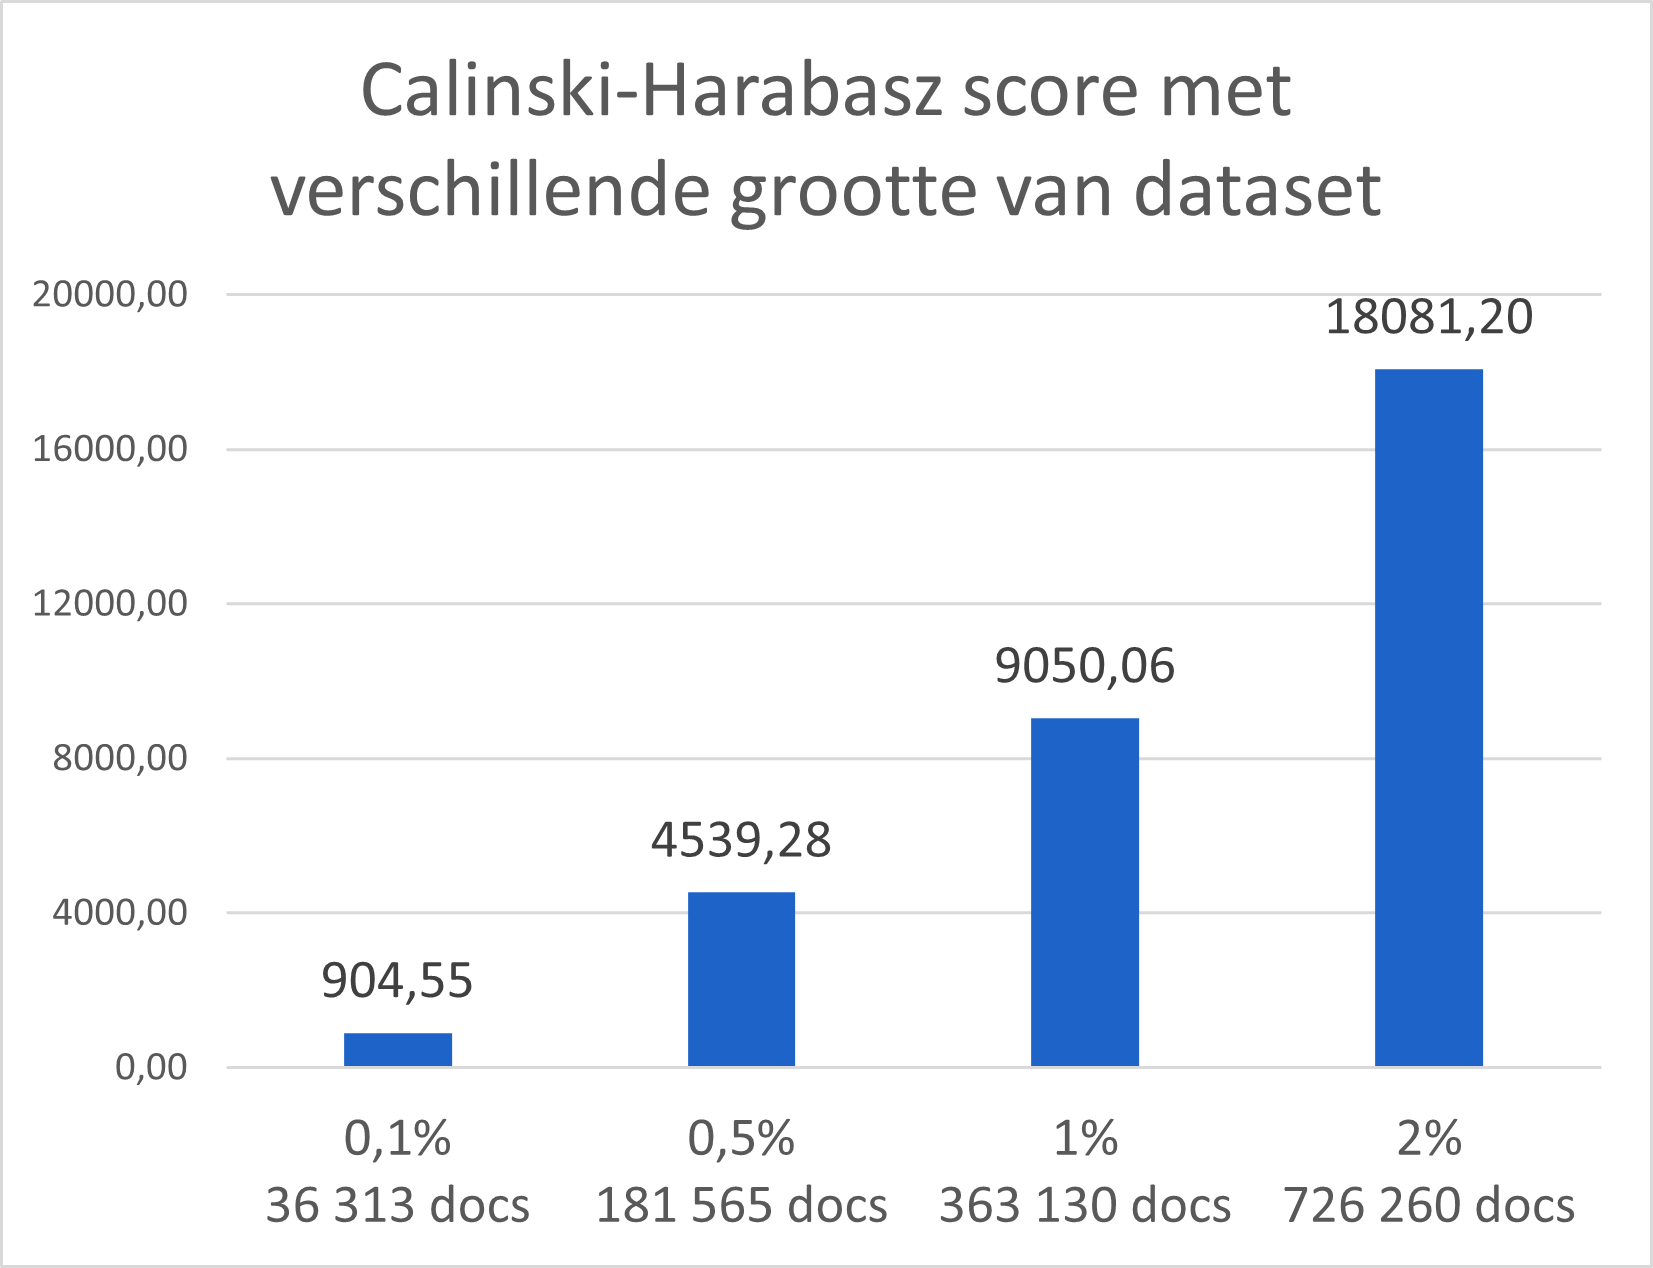
\includegraphics[width=1\linewidth]{fig/chapt4/NLP/cal_data.png}
    \end{subfigure}
    \begin{subfigure}{.5\textwidth}
        \centering
        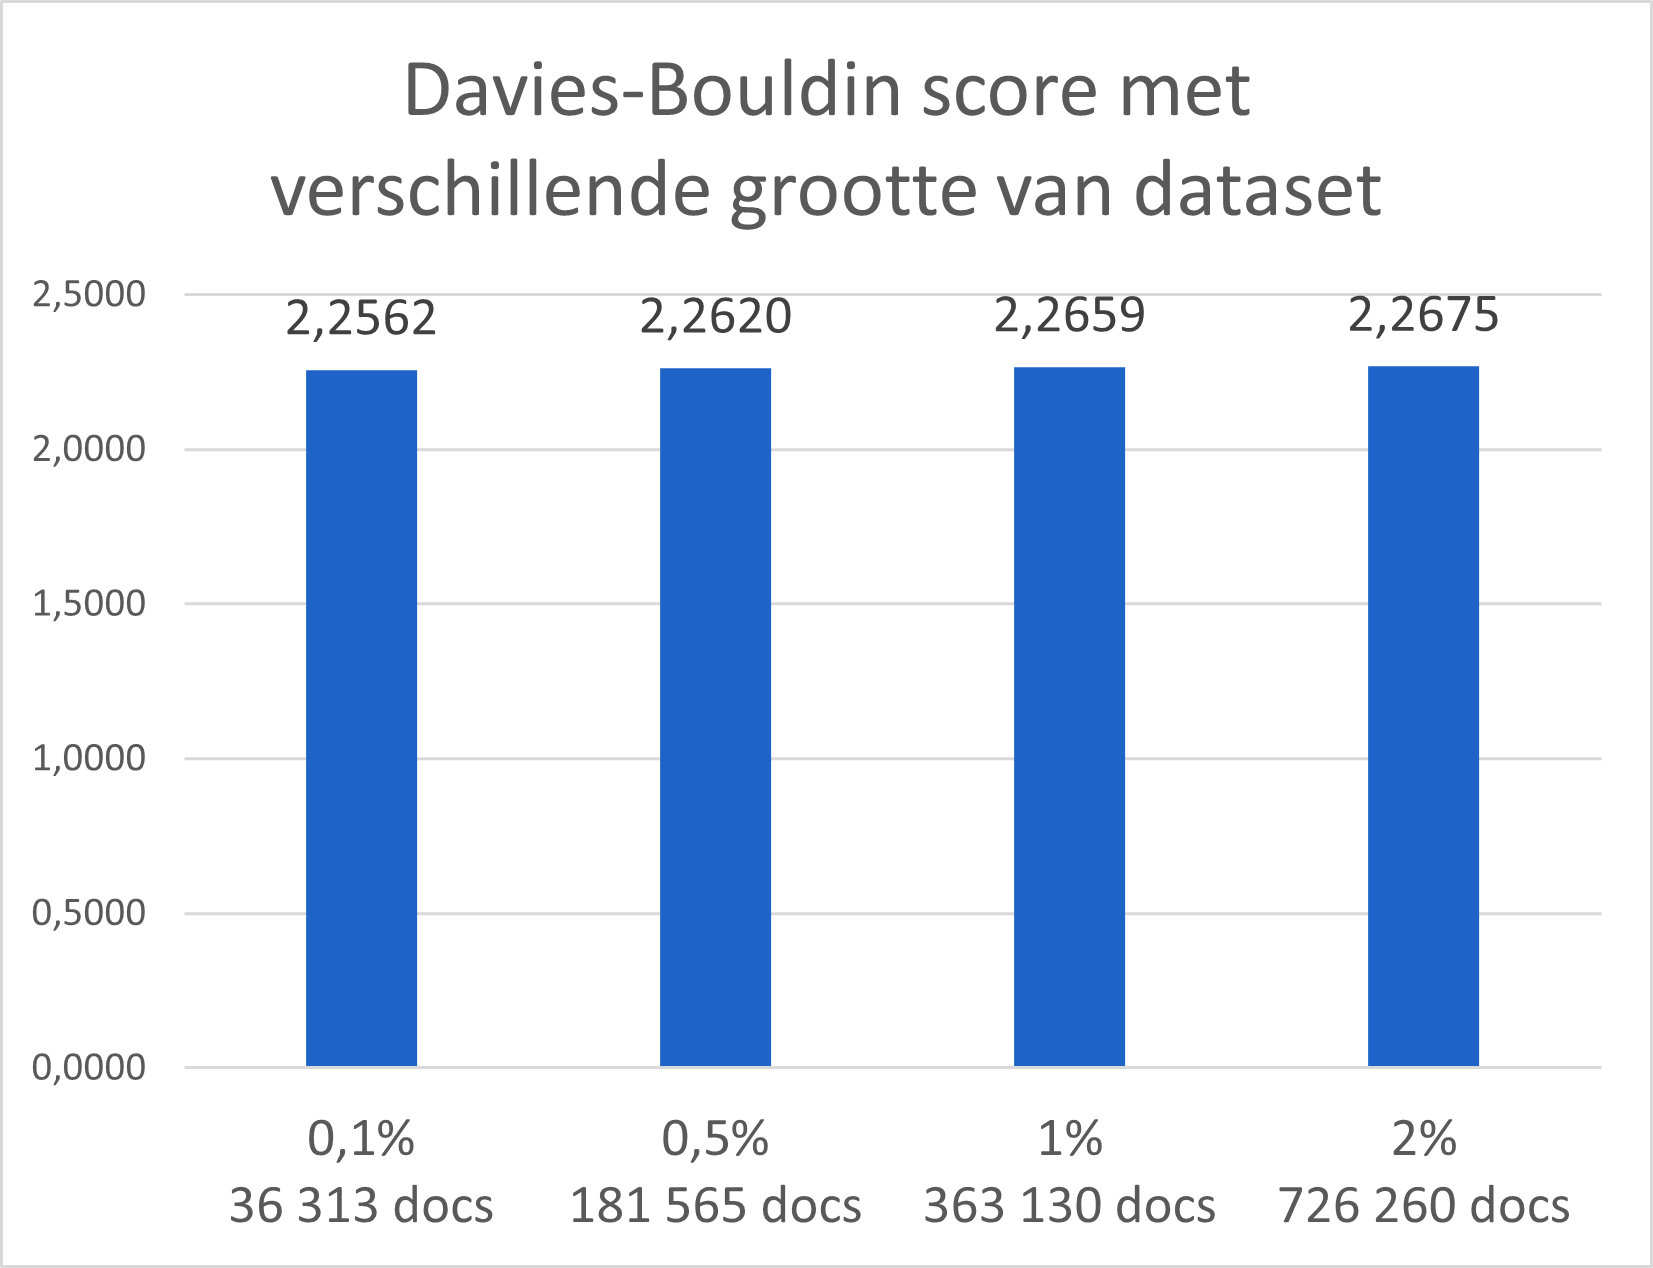
\includegraphics[width=1\linewidth]{fig/chapt4/NLP/davies_data.png}
    \end{subfigure}
    
    \centering
    \begin{subfigure}{.5\textwidth}
        \centering
        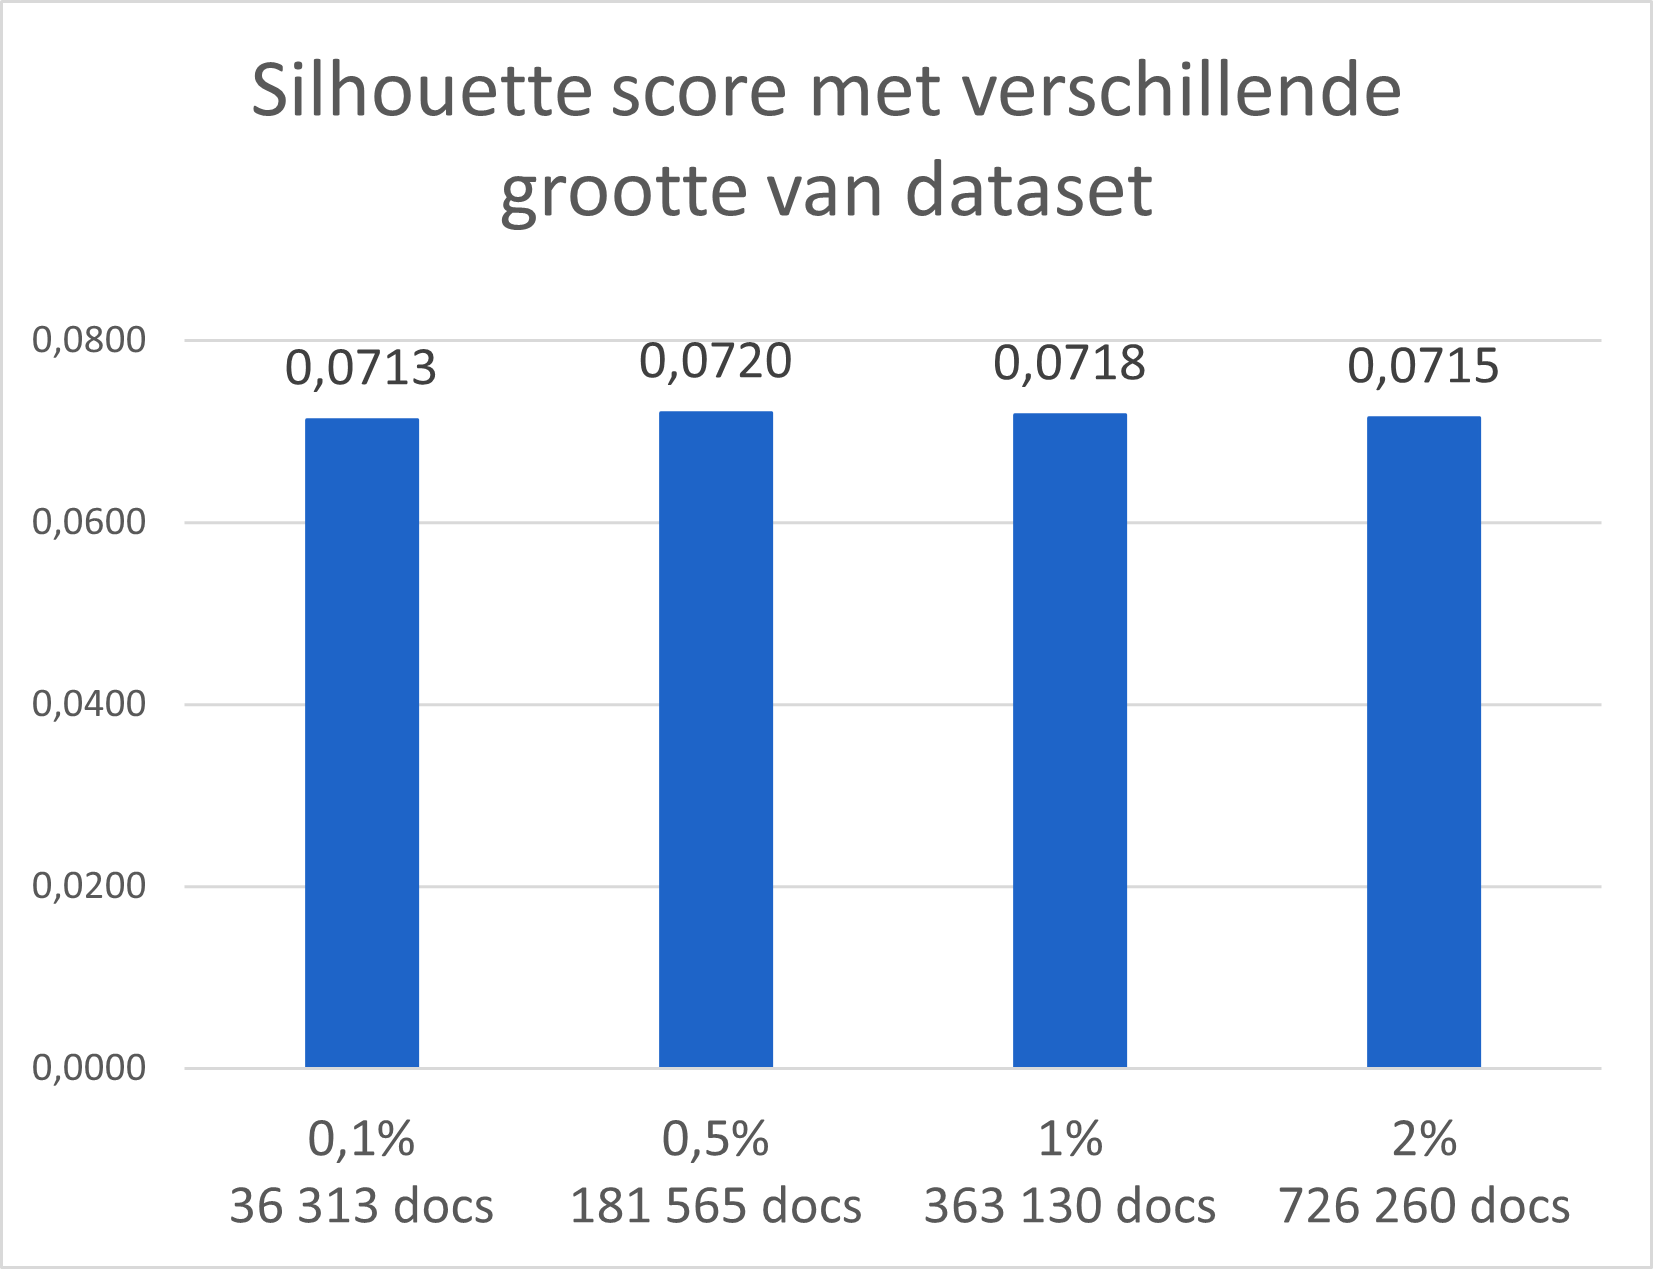
\includegraphics[width=1\linewidth]{fig/chapt4/NLP/silhouette_data.png}
    \end{subfigure}
    \caption{De scores van het model online\_50, voor verschillende groottes van de dataset}
    \label{fig:chapt4_datapercentage_clusteringmetrics}
\end{figure}

In \autoref{fig:chapt4_datapercentage_clusteringmetrics} zijn de scores weergegeven voor $0,1\%$, $0,5\%$, $1\%$ en $2\%$ van de dataset. We kunnen waarnemen dat er geen significante verschillen zijn voor de Davies-Bouldin score en silhouette score. Voor de Calinski-Harabasz score zien we een lineaire stijging die afhangt van de hoeveelheid data. Deze stijging is te verklaren door het gebruik van het aantal datapunten in de formule. Doordat de metrieken de eigenschappen van de clusters modelleren, concluderen we dat er geen significante verschillen tussen de clusterings zijn bij verschillende datagroottes, en dat de metrieken over een subset van de datapunten representatief zijn voor alle datapunten. In de volgende vergelijkingen gebruiken we daarom enkel de scores van $1\%$ van de data. 

\begin{figure}[H]
    \begin{subfigure}{.5\textwidth}
        \centering
        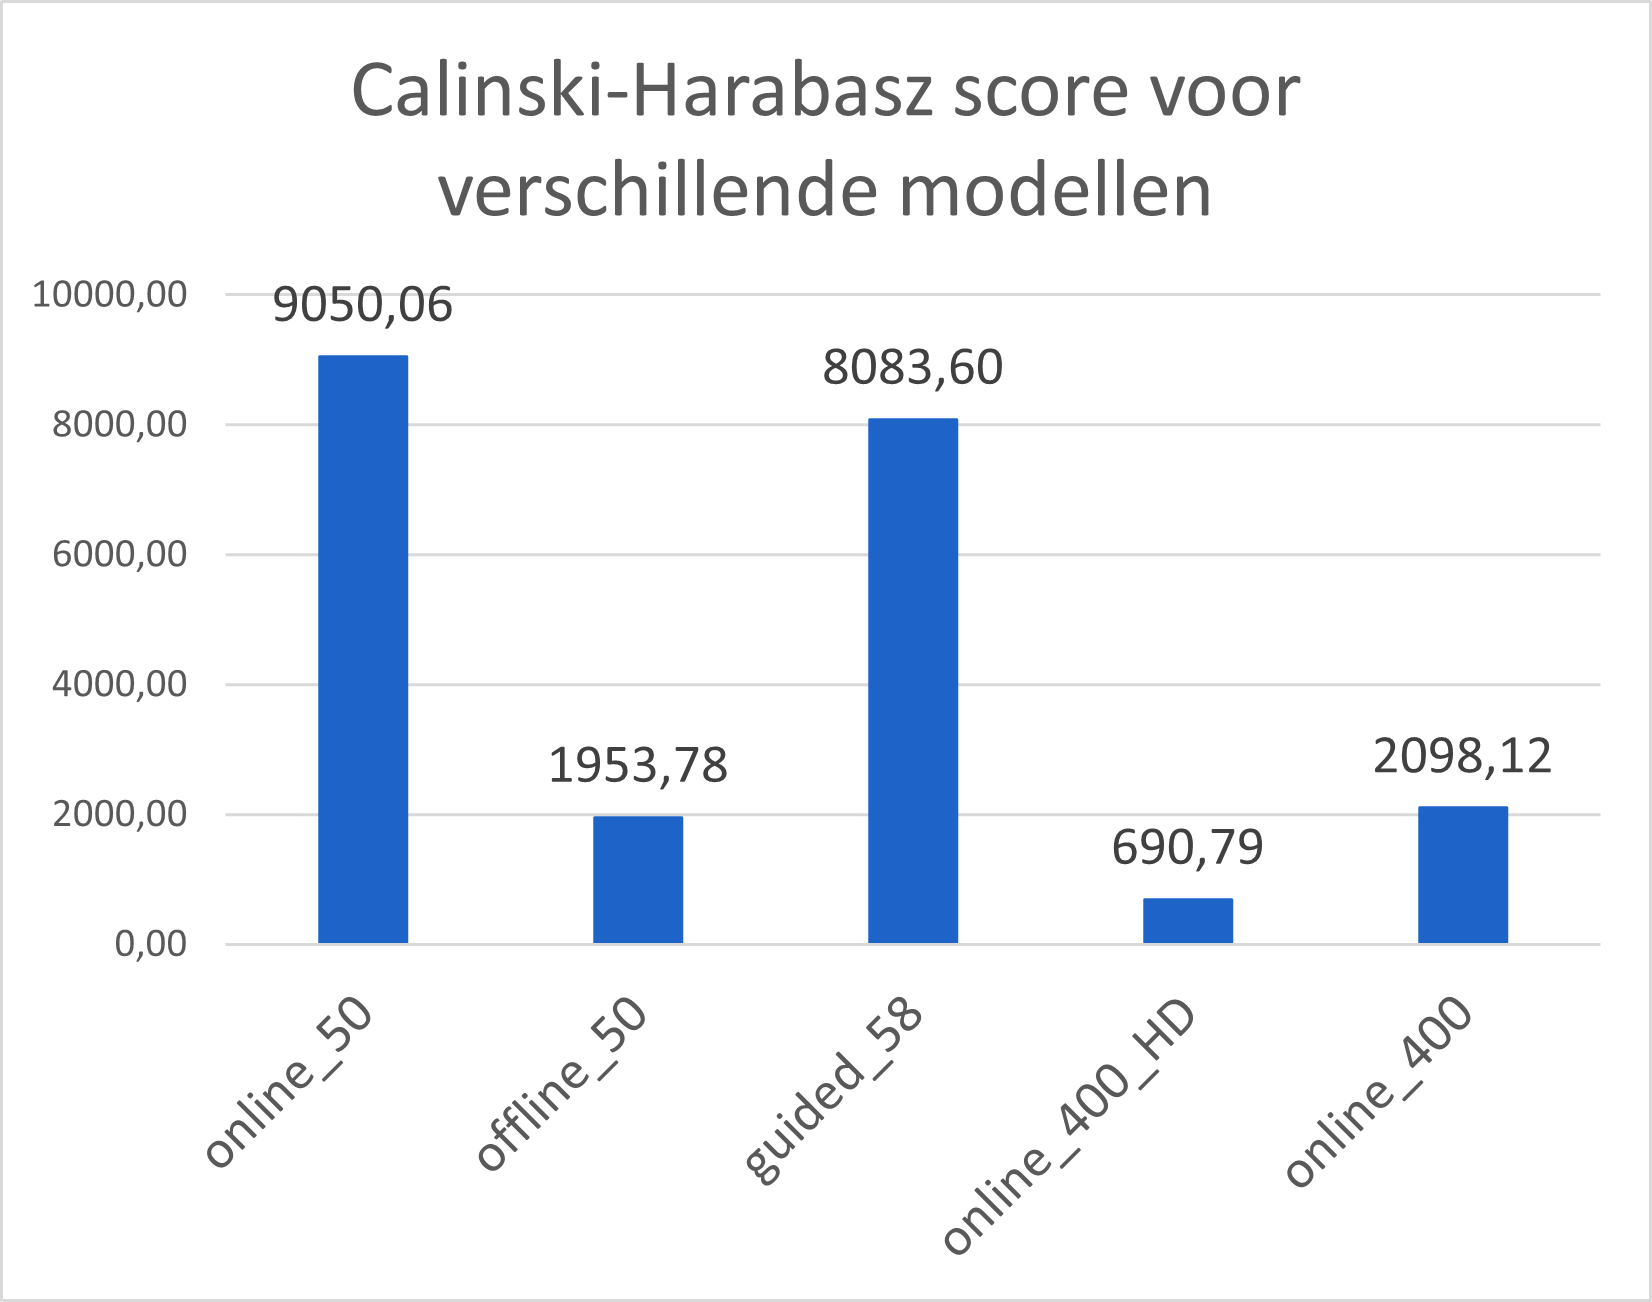
\includegraphics[width=1\linewidth]{fig/chapt4/NLP/cal_model.png}
    \end{subfigure}
    \begin{subfigure}{.5\textwidth}
        \centering
        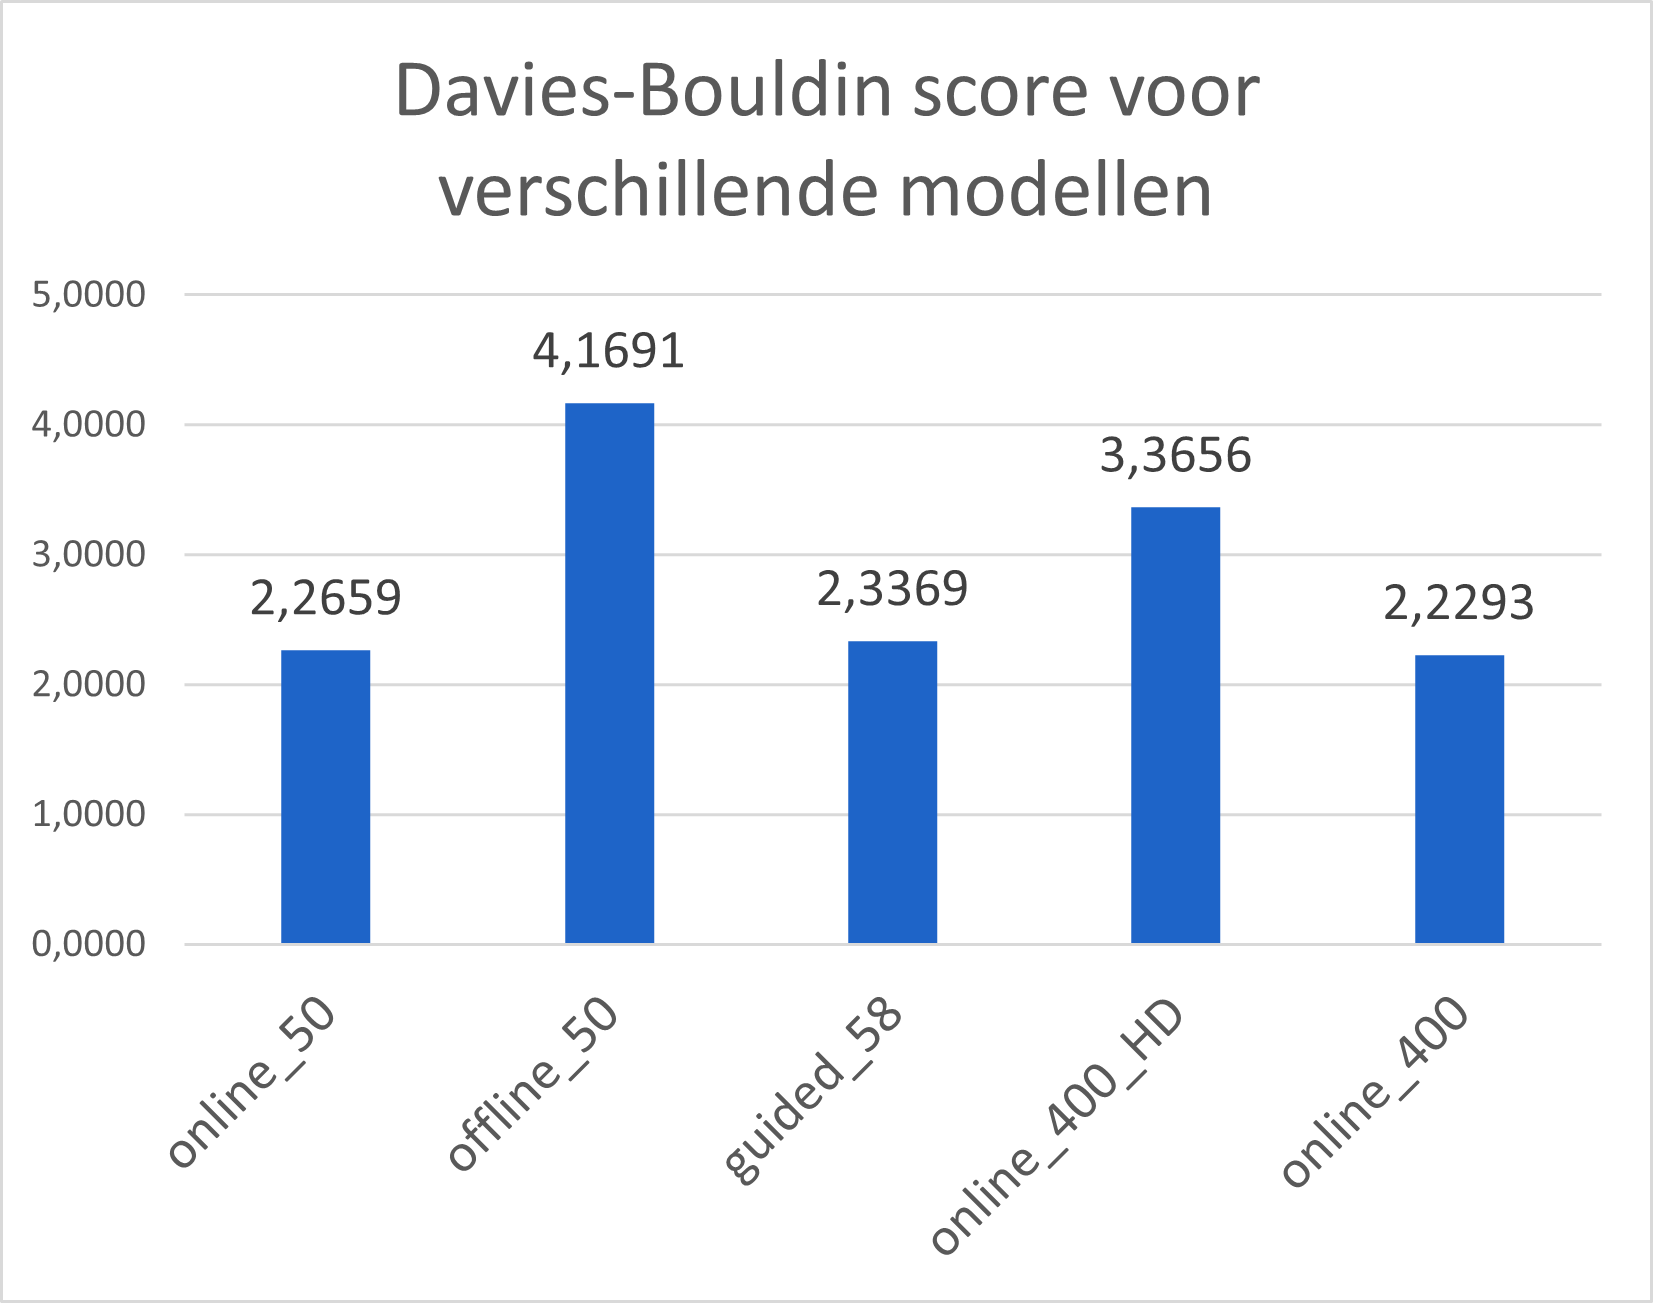
\includegraphics[width=1\linewidth]{fig/chapt4/NLP/davies_model.png}
    \end{subfigure}
    
    \centering
    \begin{subfigure}{.5\textwidth}
        \centering
        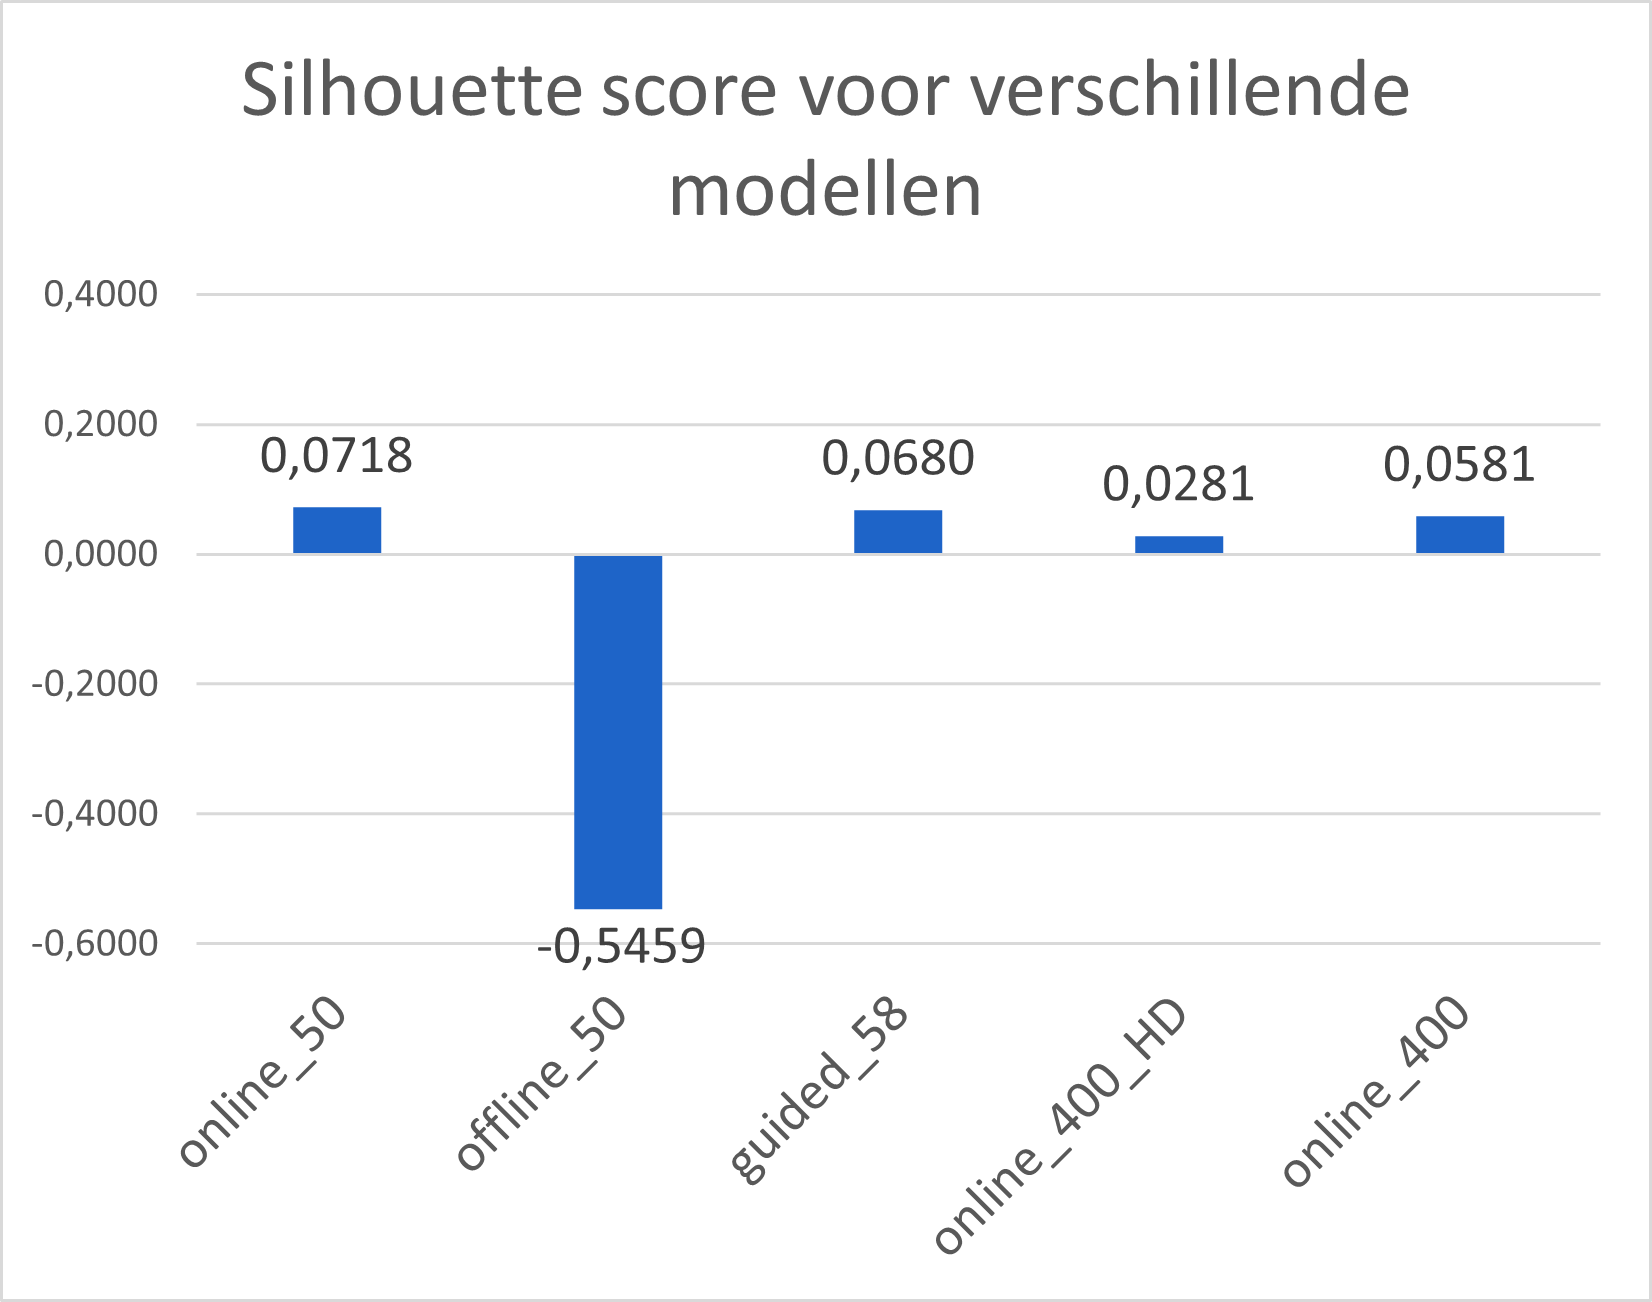
\includegraphics[width=1\linewidth]{fig/chapt4/NLP/silhouette_model.png}
    \end{subfigure}
    \caption{Scores voor de verschillende modellen (1\% van dataset)}
    \label{fig:chapt4_clusteringmetrics_vergelijking}
\end{figure}
% TODO: eventueel bij de laatste grafiek de as Y=0 iets vetter zetten, zodat het duidelijker is dat offline een negatieve score heeft

% online_50, online_400 en guided_58 hebben beste score (dunn/silhouette)
% offline doet significant slechter
% meer dim houden doet ook slechter maar kan aan dim reduction liggen
Uit \autoref{fig:chapt4_clusteringmetrics_vergelijking} kunnen we het volgende concluderen: de volgende modellen hebben algemeen de beste scores: online\_50, online\_400 en guided\_58\footnote{\q{online\_50} wil zeggen \q{Online BERTopic, 50 topics}, etc}. Voor deze modellen liggen de Davies-Bouldin score en silhouette score dicht bij elkaar. De exacte volgorde verschilt afhankelijk van de gekozen metriek. In het geval van Calinski-Harabasz score zijn er verschillen, maar deze linken we aan het verschillend aantal topics per model.\newline
Het vierde beste model is online\_400\_HD waarbij de dimensionaliteitsreductie meer dimensies behoudt. Hierbij zien we dat de silhouette score iets slechter is, maar de Davies-Bouldin score significant hoger en dus slechter is. Voor de Calinski-Harabasz score kunnen we het enkel vergelijken met een ander model van 400 topics, namelijk online\_400. Hierbij nemen we waar dat de score significant lager en dus slechter is. Het laatste model is offline\_50, hierbij zien we dat alle scores significant slechter zijn. Merk op dat de silhouette score zelfs sterk negatief is wat wijst op een slechte clustering.

% todo plots kunnen ook hier (formatting)

Voor de drie beste modellen geven de scores aan dat de clustering niet optimaal is, maar dit betekent niet dat er een betere clustering is. Deze metrieken moeten we vooral gebruiken om verschillende clusteringsalgoritmen te vergelijken. Een potentiële verklaring kan zijn dat sentence-BERT, het model gebruikt voor de embeddings te generen, getraind is op algemene data en dus niet is gefinetuned op restaurantsdata. Hierdoor is het mogelijk dat het model de embeddings voor eten, service en andere restaurant gerelateerde termen te dicht bij elkaar zal leggen. Het gevolg hiervan is dat de uiteindelijke clustering veel overlap zal hebben, wat een verklaring kan zijn voor een niet optimale clustering.

Ten slotte vermelden we nog dat de evaluatie van clustering alleen niet volstaat om de uiteindelijke gebruikers- en restaurantprofielen te beoordelen. Dit komt omdat bepaalde delen, zoals sentiment analysis, onafhankelijk zijn van het gebruikte BERTopic model. We zullen in \autoref{sub:chapt5_compare_eval_methods} wel analyseren of er een verband is tussen de beste profielen en de beste modellen volgens de clusteringsmetrieken.


\subsection{Gebruikers- en restaurantprofielen}
\label{sec:chapt4_nlp_profielen}
De uiteindelijke features die we in het neuraal netwerk gebruiken, worden opgesteld op basis van het BERTopic-model. Deze features bestaan uit een vector voor elke gebruiker en elk restaurant, we noemen ze respectievelijk gebruikers- en restaurantprofielen. Het BERTopic-model zelf maakt gebruik van de volledige dataset om de mogelijke topics te bepalen. Dit betekent niet dat de profielen dit ook doen: deze worden met een deel van de data opgesteld, zoals beschreven in \autoref{sec:chapt4_data_flow}.\newline
Het opstellen kan op twee manier gebeuren. De eerste manier spreekt voor zich: deze maakt simpelweg gebruik van het model door de clusters per review te bepalen en op basis daarvan een profiel op te stellen. De andere manier zal geen gebruik maken van de clustering: hierbij zal een profiel afleid worden uit de topic representaties van het getrainde BERTopic-model. Ten slotte maken we een onderscheid bij het opstellen van gebruikers- en restaurantprofielen: de stappen om het profiel op te stellen kunnen licht wijzigen door bijvoorbeeld sentiment analysis toe te passen.

\subsubsection{Profiel op basis van de clustering}
\label{sub:chapt4_profile_by_clustering}
% VIA CLUSTERING
% clusters ci bepalen voor elke zin => CACHED
% tellen hoeveel keer elke cluster gekozen werd per user:
% TOEVOEGING sentiment: positief/negative => +1 en -1 of gewogen via de confidence score -> performance met/zonder (MOET via neuraal netwerk)
% groupby reviews => KEUZE normalizeren VS later doen -> elke review evenveel impact vs elke zin evenveel impact
% indien genormalizeerd => gemiddelde nemen van alle reviews van de user => elke review heeft evenveel impact
% indien niet genormalizeerd => alles sommeren en dan normalizeren => gevolg is dat elke zin evenveel impact heeft.
De eerste stap van deze methode is het verkrijgen van de clustering. We gaan voor elk document $d_i$ een cluster $c_j$ toekennen aan de hand van het model met $k$ clusters zoals afgebeeld in \autoref{fig:chapt4_documents_to_clustering}, waarbij $0 \le j < k$.

\mijnfiguur[H]{width=12cm}{fig/chapt4/NLP/documents_to_clustering.jpg}{Het bepalen van de clustering van de documenten door de bevraging van een getraind BERTopic model.}{fig:chapt4_documents_to_clustering}

Om vervolgens een profiel op te stellen, bepalen we de meest voorkomende onderwerpen. We moeten dus deze clusterinformatie aggregeren per gebruiker of restaurant. Hiervoor gaan we eerst de clusters $c_j$, verkregen per zin, samenvoegen tot een vector $R_r$ die de clustering van één review $r$ zal voorstellen. We doen dit door een vector van lengte $k$, met $k$ het totaal aantal clusters van het gebruikte model, op te stellen. Elk element $x_j$, met $0 \le j < k$, komt overeen met het aantal voorkomens van $c_j$ bij de zinnen van de review. Voor de reviewvector voor review $r$ geldt dan:

\begin{equation}
\label{eq:chapt4_profile_per_review}
    R_r = [x_{r0}, x_{r1}, ..., x_{rk}]
\end{equation}

Een variant hierop kan gegenereerd worden door gebruik te maken van sentiment analysis. Om dit te realiseren, bepalen we voor elk document $d_i$ of de sentiment positief, neutraal of negatief is, voorgesteld door de sentimentscore $s_i \in [-1, 1]$. De aanwezigheid van een topic $c_j$ in document $d_i$ wordt dan vermenigvuldigd met $s_i$. Na het aggregeren kan een bepaald onderwerp dan een negatieve score krijgen. Waarom dit nuttig kan zijn, wordt beschreven in \autoref{sub:chapt4_users_vs_restaurants}.

We hebben op dit punt een vectormodel opgesteld voor elke review. We kunnen deze vectoren nu aggregeren tot één profiel per gebruiker of restaurant. We doen dit door de vectoren van alle reviews van één bepaalde gebruiker of restaurant elementsgewijs op te tellen. Voor gebruiker $u$ nemen we de som van alle vectoren van de reviews geschreven door $u$. Ten slotte zullen we deze geaggregeerde vector normaliseren zodat alle waarden in het interval $[0, 1]$ liggen. Dit proces is formeel uitgedrukt in \autoref{eq:chapt4_profile_per_user}. We kunnen dit analoog doen voor een restaurantsprofiel: we sommeren over de vectoren van alle reviews die geschreven zijn over het bepaalde restaurant.

\begin{equation}
\label{eq:chapt4_profile_per_user}
    UP_{u} = normalize(\sum_{R \in Reviews_u}R)
\end{equation}

Aan de hand van bovenstaande methode zal elke zin evenveel impact hebben op het uiteindelijke profiel. Dit is niet optimaal, want één review beschrijft één bezoek aan een restaurant. De lengte van die review vertelt niets over de belevenis van de gebruiker. Het probleem is dat de vectoren $R$ van reviews met meer zinnen zwaarder doorwegen doordat er gesommeerd wordt per zin.\newline
Hierdoor is het logischer om te zorgen dat elke review evenveel impact maakt op een profiel, in plaats van elke zin.  Dit probleem wordt opgelost door elke vector $R$ te normaliseren zoals beschreven in \autoref{eq:chapt4_profile_per_review_normalized}. Het gevolg hiervan is dat elke review een even grote impact heeft op het uiteindelijke profiel.

\begin{equation}
\label{eq:chapt4_profile_per_review_normalized}
    R_r = normalize([x_{r0}, x_{r1}, ..., x_{rk}])
\end{equation}

\subsubsection{Profiel op basis van de representaties}
\label{sub:chapt4_profile_repesentaties}
% VIA APPROXIMATION
% uit de representaties van de cluster VS document (MERK OP DAT DIT OOK KAN PER REVIEW, wij hebben het per zin gedaan (sommige zinnen meerdere onderwerpen)  => CACHED
% estimaties voor elke topic = SOM is 1
% neem de beste N per topic (door de anderen op 0 te zetten)
% OPTIONELE STAP -> normalizatie zodat de som van deze topics 1 is
% analoog aggregeren per review en dan per user/restaurant
% ten slotte het elk profiel normalizeren (tussen 0-1)

% voordeel => NOG meer topics per zin!
Deze methode maakt geen gebruik van de clustering, maar van de representatie van de topics van het model. Hierbij zal men elk document $d_i$ opsplitsen in meerdere groepen van woorden aan de hand van een sliding window. Vervolgens gaat men voor elke groep de c-TF-IDF-representatie berekenen en bekijken hoe gelijkaardig deze zijn aan de mogelijk topicrepresentaties van het model zelf. Deze vergelijking zal gebeuren via de cosinusgelijkenis. Hierna zal men alle groepen elementsgewijs sommeren en ten slotte normaliseren zodat de som van de elementen van de vector gelijk is aan $1$. De uiteindelijke output is een genormaliseerde vector $A$ met lengte $k$, waarbij $k$ het aantal clusters van het model is. Hierbij stelt de waarde $A_j$ de relevantie van topic $c_j$ voor, deze waarde is relatief tegenover de andere topics.

\mijnfiguur[H]{width=12cm}{fig/chapt4/NLP/documents_to_approximation.jpg}{Het bepalen van een approximatie voor de documenten door gebruik te maken van de representaties van een getraind BERTopic model.}{fig:documents_to_approximation}

Bij de verschillende BERTopic-modellen heeft $k$ een verschillende waarde, hierdoor zullen de waarden in de vector $A$ kleiner/groter zijn wegens een grotere/kleinere spreiding. Aangezien we elk profiel met een gelijkaardige impact per review willen opstellen, zullen we elke vector $A$ aanpassen. We doen dit door de $n$ hoogste waarden bij te houden en de overigen gelijk te stellen aan nul. Vervolgens zullen we deze vector normaliseren zodat elke waarde in het interval $[0,1]$ ligt, hierdoor zal de impact niet afhangen van de lengte van de vector. Dit proces is beschreven in \autoref{eq:chapt4_approx_normalize_sentence_profile}. 

\begin{equation}
AN = normalize([an_0, an_1, ..., an_k]) \;\;\;\;\;\;\;
\label{eq:chapt4_approx_normalize_sentence_profile}
\begin{cases}
    an_i = a_i, & \text{als } a_i \in \text{top n}  \\
    an_i = 0,   & \text{anders}
\end{cases}
\end{equation}

Met deze aangepaste vectoren $AN$ kunnen we de reviewprofielen opstellen. We zullen dit doen door elementsgewijs de som te nemen van elke $AN_i$ overeenkomend met de zinnen van de review. Deze reviewprofielen gaan we ook normaliseren zodat elke review evenveel impact heeft. Formeel stellen we dat:

\begin{equation}
\label{eq:chapt4_profile_per_review_approx}
    RA_{r} = normalize(\sum_{zin \in R_r}AN_{zin})
\end{equation}

Bij deze reviewprofielen kunnen we ook sentiment analysis toevoegen op een analoge manier zoals in \autoref{sub:chapt4_profile_by_clustering}. Ten slotte zullen we de gebruikers- en restaurantprofielen opstellen door de reviewprofielen te aggregeren. Dit zal analoog gebeuren als in \autoref{sub:chapt4_profile_by_clustering} aan de hand van \autoref{eq:chapt4_profile_per_user}.

\subsubsection{Gebruikers tegenover restaurants}
\label{sub:chapt4_users_vs_restaurants}
In de vorige secties haalden we verschillende mogelijkheden aan om gebruikers- en restaurantprofielen op te stellen. Voor de meeste parameters is er weinig tot geen verschil tussen een profiel opstellen voor een gebruiker tegenover een restaurant. Dit geldt ook voor de algoritmes op basis van clustering en representaties.

De meest interessante onderzoeksparameter is het gebruik van sentiment analysis. Beschouw het volgende voorbeeld:\newline
een gebruiker gaat naar een pizzarestaurant. De gebruikerservaring was negatief aangezien de pizza niet lekker was. Hierdoor is de sentiment analysis van de review negatief. Indien we dit toevoegen aan een gebruikersprofiel zou dit weergeven dat een gebruiker pizza niet lekker vindt. Deze assumptie komt niet overeen met de realiteit, aangezien de gebruiker een pizzarestaurant bezocht, nemen we aan dat hij pizza lekker vindt. Hierdoor is het logisch om geen sentiment analysis toe te passen bij een gebruikersprofiel. \newline
Beschouw hetzelfde voorbeeld voor een pizzarestaurant dat, wat betreft het eten, meerdere negatieve reviews heeft gekregen. In dit geval zouden negatieve scores in het restaurantprofiel voorstellen dat de pizza niet lekker is. Dit komt dus wel overeen met de realiteit dat gebruikers de pizza niet smaakvol vinden, zoals beschreven in de reviews. Hierdoor zullen we bij het opstellen van een restaurantprofiel wel gebruik maken van sentiment analysis.

% TODO: wat hieronder staat is niet nagelezen
% restaurant: goed/slecht -> 'fabulous', 'awful', ...
% restaurant: hoe was het eten -> 'overcooked', 'seasoned', ...
Een ander verschil is de relevantie van de verschillende onderwerpen, hierbij laten we de topics die geen enkele relevantie hebben zoals 'wow' en 'lol' buiten beschouwing. Voor gebruikers nemen we een subset van de restaurants, alles wat voor een gebruiker relevant is zal ook van toepassing zijn bij een restaurant. In de omgekeerde richting geldt dit niet. De onderwerpen die vooral woorden zoals 'verschrikkelijk gekruid' en 'aangebrand' bevatten, gaan over het eten in het restaurant. Weten dat een gebruiker geen aangebrand eten wil, levert geen bijdrage op aangezien dit te algemeen is. Voor diezelfde reden kunnen we ook de algemene termen zoals 'super', 'goed', 'slecht' uitsluiten bij gebruikersprofielen. Hierdoor zal een restaurantsprofiel dus uit meer topics bestaan. Merk op dat deze verdeling volledig manueel gedaan moet worden, hierdoor is deze uiterst subjectief en vatbaar voor menselijke fouten.

% TODO is het restaurantprofiel of restaurantsprofiel -> mogelijk niet overal consistent!

























































\section{Neuraal netwerk}
\label{sec:chapt4_neuraal_netwerk}

% TODO: waarom een neuraal netwerk? Welke voordelen spreken ons aan?
% TODO: Arno, go ahead. Bespreek in deze section ook al de individuele resultaten. Random grafieken: go! Chapter 5 is enkel bedoelt om alles nog eens samen te vatten
\subsection{Input}
Zoals aangeduid in \autoref{fig:chapt4_architectuur_begin} zijn er twee bronnen van inputdata voor het neuraal netwerk: de labels rechtstreeks geëxtraheerd uit de Yelp dataset, en de geschreven reviews die zijn omgezet naar numerieke features zoals beschreven in \autoref{sec:chapt4_nlp_profielen}. Beide bronnen modelleren steeds zowel een gebruikerprofiel als een restaurantprofiel. Met deze data moet het neuraal netwerk een voorspelling maken welke score die specifieke gebruiker aan dat specifieke restaurant geeft. Merk op dat deze profielen worden opgesteld met slechts een deel van de train- of testset, zoals beschreven in \autoref{sec:chapt4_data_flow} % TODO: een zelfde soort 'warning' bij Arnoud zijn deel zetten

Een neuraal netwerk aanvaardt enkel numerieke features. Bij de NLP gebruikers- en restaurantprofielen is dit reeds opgelost. Bij de labels is er meer werk. We bespreken eerst hoe een restaurant gemodelleerd wordt, en daarna hoe we deze modellering kunnen aanpassen om ook gebruikersdata te ondersteunen.
% TODO: checken dat er niet te veel overlap is met Arnoud hier
\subsubsection{Restaurantlabels}
\label{sec:chapt4_nn_restaurantlabels}
Een restaurant wordt hoofdzakelijk beschreven in de Yelp dataset met behulp van categorieën en attributen (\autoref{sec:chapt3}). We maken gebruik van one-hot encoding om de aanwezigheid van een categorie (nominaal) bij een restaurant aan te duiden. Doordat er in de totale dataset 1311 unieke categorieën zijn, zou er door de one-hot encoding een zeer ijle inputvector gemaakt worden. Om dit probleem te beperken, houden we enkel de categorieën die bij minstens 500 restaurants (1\% van totaal) voorkomen. Zo houden we nog 75 categorieën over.

Niet ieder restaurant beschikt over een waarde voor ieder attribuut. Ongeveer 33\% van de restaurants ontbreekt minstens één attribuut. Ordinale data, zoals de prijsklasse, wordt omgezet naar een waarde in $[0, 1]$ die overeenkomt met de rangorde. Voor de andere attributen gebruiken we opnieuw one-hot encoding. In tegenstelling tot categorieën moeten we rekening houden dat de afwezigheid van een attribuut in de dataset niet per se overeenkomt met het werkelijk ontbreken van dat attribuut in de echte wereld. Aangezien deze data wel waardevol lijkt voor aanbevelingen, lossen we dit probleem op door een standaardwaarde per attribuut in te stellen. Zo wordt de afwezigheid van een one-hot encoded attribuut gemodelleerd als $0,5$.

We berekenen de huidige gemiddelde score van een restaurant en voegen deze toe als feature. De Yelp dataset bevat ook de check-ins voor ieder restaurant. Deze datapunten worden omgezet tot een numerieke waarde door het gemiddeld aantal check-ins per week te berekenen. Samen modelleren deze twee nieuwe features een rudimentaire vorm van de populariteit van een restaurant.

Het gemiddeld aantal check-ins per week bij een restaurant varieert sterk, van quasi 0 bij niche restaurants tot meer dan 100 bij grote ketens. Deze afgeleide feature ligt dus niet in $[0, 1]$ zoals alle andere features en zou ervoor zorgen dat deze feature meer doorweegt in het neuraal netwerk. De spreiding van waarden van deze feature is ook niet uniform: er zijn enkele uitschieters die niet in lijn liggen met de overige restaurants. Een gewone normalisatie zal dit dus niet oplossen. We herschalen daarom alle data die tussen het 5$^e$ en 95$^e$ percentiel tot $[0, 1]$ en extreme lage en hoge waarden transformeren we tot respectievelijk $0$ en $1$. Hierdoor krijgen we een betere spreiding en heeft deze feature een even groot gewicht als alle andere.

\subsubsection{Gebruikerslabels}
Uit \autoref{sec:chapt4_nn_restaurantlabels} volgt dat we een restaurant $i$ kunnen voorstellen aan de hand van labels in de vorm van een vector $RP_i = (feature_1, feature_2, ..., feature_n)$. We bepalen nu per gebruiker de verzameling van restaurants $\mathcal{V}$ waarvoor die gebruiker een review heeft achtergelaten. We kunnen dan voor gebruiker $j$ een gebruikersprofiel $UP_j$ opstellen:
\begin{equation}
    UP_j = \frac{\sum_{v \in \mathcal{V}} (RP_v \cdot R_{j, v})}{\vert \mathcal{V} \vert}
\end{equation}

met $R_{j, v}$ de genormaliseerde score die gebruiker $j$ geeft aan restaurant $v$. De Yelp dataset bevat nog enkele andere gegevens over de gebruikers: zo wordt er bijgehouden hoeveel keer andere gebruikers een review 'nuttig', 'grappig' of 'cool' vonden. Deze metadata over een gebruiker helpt om de betrouwbaarheid van de reviews te modelleren. We creëren een nieuwe feature door de som van het aantal positieve interacties te nemen. Er zijn enkele bekende gebruikers op Yelp die veel volgers hebben en hierdoor veel meer feedback hebben gekregen op hun reviews. Daarom herschalen we eerst de feature door alle waarden hoger dan het 99$^e$ percentiel te mappen op $1$ en de rest te normaliseren tussen $[0, 1]$.

Beide profielen, gecombineerd met de profielen die gecreëerd zijn aan de hand van NLP, vormen de input voor het neuraal netwerk. (\autoref{fig:chapt4_architectuur_input})

\mijnfiguur[H]{width=8cm}{fig/chapt4/predictor/architectuur_input.png}{Close-up inputlaag van architectuur zoals in \autoref{fig:chapt4_architectuur_begin}}{fig:chapt4_architectuur_input}


% TODO: zie correlatiegraphs, om te bekijken of er obvious dubbele data inzit of niet
% TODO: zeggen dat corr. voor andere NLP profielen er basically zelfde uitziet

\subsubsection{Correlaties}
Het lijkt overbodig om zowel de labels als geschreven reviews te verwerken in hetzelfde neuraal netwerk, daar deze dezelfde objecten omschrijven. We beschouwen een paar features $(f_i, f_j)$ gecorreleerd indien $\lvert C(f_i, f_j) \rvert \ge 0,70$. Intuïtief zou men denken dat er sterke correlaties bestaan tussen een overeenkomstig profiel opgesteld door NLP en aan de hand van labels.\newline
Dit blijkt echter niet het geval: er zijn maar 14 van de 495 510 paren van features waarbij de absolute waarde van de correlatie groter is dan $0,70$. Nog opmerkelijker: deze correlaties treden enkel op binnenin eenzelfde databron, en niet tussen NLP en labels. We besluiten hieruit dat de NLP-profielen andere informatie extraheert dan de gelabelde dataset aanbiedt.

\begin{figure}[H]
    \begin{subfigure}{.5\textwidth}
        \centering
        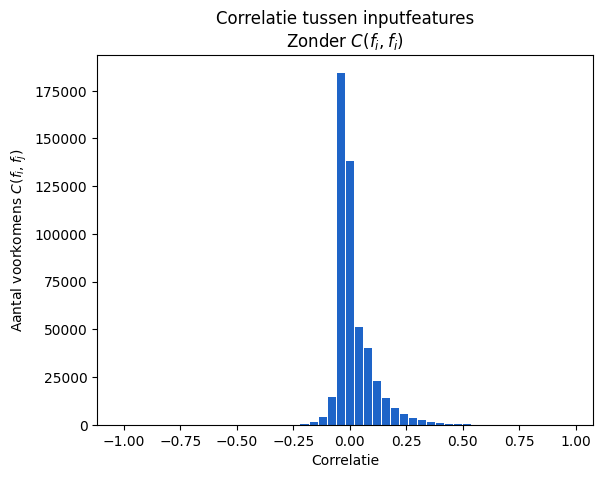
\includegraphics[width=1\linewidth]{fig/chapt4/NLP/correlaties_input.png}
        \caption{Histogram correlaties tussen inputfeatures}
        \label{fig:chapt4_correlaties_input}
    \end{subfigure}
    \begin{subfigure}{.5\textwidth}
        \centering
        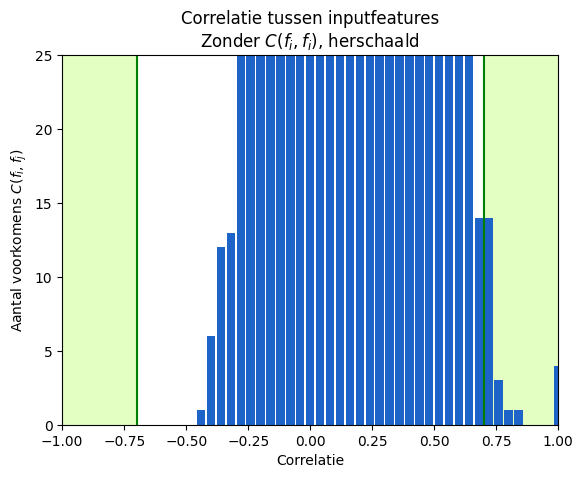
\includegraphics[width=1\linewidth]{fig/chapt4/NLP/correlaties_input_herschaald.png}
        \caption{Histogram correlaties tussen inputfeatures, herschaald voor randwaarden}
        \label{fig:correlaties_input_herschaald}
    \end{subfigure}
    \caption{Analyse correlaties inputfeatures}
    \label{fig:chapt4_correlaties_combined}
\end{figure}

\begin{table}[H]
    \centering
    \begin{tabular}{l|l}
    Feature 1 & Feature 2 \\ \hline
    restaurant category nightlife & restaurant category bars \\
    restaurant category event planning \& services & restaurant category caterers \\
    restaurant category beer & restaurant category wine \& spirits \\
    restaurant category music venues & restaurant category arts \& entertainment \\
    restaurant NLP profile 37 & restaurant NLP profile 17 \\
    restaurant NLP profile 323 & restaurant NLP profile 180 \\
    user compliments & user fans \\
    user positive interactions & user fans \\
    user positive interactions & user compliments \\
    user category nightlife & user category bars \\
    user category japanese & user category sushi bars \\
    user category event planning \& services & user category caterers \\
    user category beer & user category wine \& spirits \\
    user category music venues & user category arts \& entertainment \\
    \end{tabular}
    \caption{Paren van features waarbij de absolute waarde van de correlatie groter is dan $0,70$}
    \label{}
\end{table}

De volledige data is beschikbaar in \verb|src/corr.zip|. Deze conclusie geldt voor alle varianten van profielen gemaakt door NLP.

\subsection{Testset-up}
De modellen zijn steeds geschreven in Python 3.10. De implementaties maken gebruik van PyTorch 2.0.0. \cite{pytorch} De inputvector voor het neuraal netwerk bestaat uit \verb||torch.float32 getallen. De uitvoering gebeurt op een AMD Ryzen 5800X, NVIDIA RTX 2080, en 64GB werkgeheugen. % TODO: checken dat bij arnoud dit klopt, en eventueel checken dat arnoud ook de azure pc erop zet, want dat lijkt beter

In dit deelonderzoek evalueren we de architectuur en parameters van het neuraal netwerk. Het effect van de inhoud van de inputvectoren wordt niet verder onderzocht. Zoals besproken in \autoref{sub:chapt4_testsetup}, zijn er meerdere mogelijke combinaties voor de NLP-profielen. We kozen de beste combinatie van profielen om verder mee te experimenteren. We analyseren iedere implementatie op dezelfde manier. De data wordt verwerkt zoals beschreven in \autoref{sec:chapt4_data_flow}: iedere epoch trainen we het neuraal netwerk met een trainset en berekenen we vervolgens de loss op de testset. Als de loss meerdere epochs op rij omhoog gaat, stoppen we het trainen om overfitting te voorkomen. De gebruikte lossfunctie voor optimalisatie is de MSE.

Nadat het model volledig getraind en getest is volgens de hierboven beschreven methode, analyseren we het model aan de hand van voorspellingen zoals we ze in de praktijk zouden gebruiken: we nemen een subset van de testset om aan de hand van het model een score tussen 1 en 5 te voorspellen. We ronden hierbij de voorspelling af, zodat het domein van de voorspelde score exact overeenkomt met het domein dat een gebruiker heeft op Yelp. We maken een histogram van het verschil tussen de voorspelling en echte score toegekend door de gebruiker. Dit histogram gebruiken we als controle dat een lagere MSE overeenkomt met meer accurate voorspellingen.

\subsection{Basisimplementatie}
\label{sec:chapt4_basisimplementatie}
We beginnen met een basisimplementatie van een neuraal netwerk, om te verifiëren dat het mogelijk is om de echte score te schatten op basis van de inputdata. We werken met een standaard multilayer perceptron (feed-forward) model. De output van het model is één waarde in $[0, 1]$. We implementeren het aanbevelingssysteem dus als een regressiemodel, waarbij de output daarna herschaald wordt naar een score tussen 1 en 5. We kiezen voor de bij regressiemodellen veelgebruikte lossfunctie MSE. Deze is ook makkelijk om te zetten naar RMSE, wat vergelijken met andere onderzoeken rechtdoorzee maakt. \cite{narre, deepconn, wide_deep_learning_paper}
% TODO: eerste idee en resultaten, problemen en opmerkingen...
Het model bestaat uit 5 verborgen lagen, waarbij het aantal neurons eerst stijgt en daarna steeds halveert (\autoref{fig:chapt4_basisimplementatie}). In tegenstelling tot collaborative filtering, kan dit model wel niet-lineaire verbanden capteren. We gebruiken Stochastic Gradient Descent (SGD) als netwerkoptimizer, met een learning rate van $0,01$.

\mijnfiguur[H]{width=16cm}{fig/chapt4/predictor/basisimplementatie_netwerk.png}{Voorstelling basisimplementatie, waarbij $n$ het aantal inputfeatures voorstelt}{fig:chapt4_basisimplementatie}



\subsection{Uitbreidingen architectuur}
We blijven bij een standaard feed-forward multilayer perceptronmodel. Dit is de meest logische keuze voor deze context. Er is bijvoorbeeld geen nood aan een model met geheugen zoals LSTM daar de inputdata geen volgorde bevat. 
We onderzoeken wel het aantal lagen en het aantal neuronen per laag. Hoe complexer het netwerk, hoe meer verbanden het capteren. Echter zorgt een stijging in complexiteit van het netwerk ook voor een complexere training die meer data nodig heeft. Complexere netwerken scoren ook slechter bij explainability. Daarom voeren we experimenten uit met een eenvoudiger netwerk met maar 1 verborgen laag, tot 8 verborgen lagen. Deze netwerken volgen een analoge structuur zoals beschreven in \autoref{sec:chapt4_basisimplementatie}. Vanaf 5 verborgen lagen zal de eerste verborgen laag wel $20$\% groter zijn dan de inputlaag, om het netwerk de kans te geven om complexere verbanden te modelleren. Tussen de eerste drie verborgen lagen zit steeds een dropout-laag. Deze laag heeft een 20\% kans om een neuron op 0 te zetten en helpt zo om overfitting te voorkomen. \cite{nn_dropout} Tijdens het testen van het model worden deze dropout-lagen uitgezet.

\subsection{Optimalisaties}
\subsubsection{Netwerk-optimizer}
We onderzoeken welk effect de gekozen optimizer heeft op de loss van het netwerk. SGD is een relatief eenvoudige optimizer waarbij de learning rate constant blijft. We proberen ook ADAGRAD, omdat deze optimizer de mogelijkheid biedt om de initiële learning rate aan te passen naargelang het trainen vordert.

De lossfunctie duidt de fout aan zodat de optimzer weet hoe het netwerk aan te passen. We onderzoeken verschillende lossfuncties die gebruikt worden tijdens het trainen, en analyseren of het resulterende model beter presteert. Het idee is dat met een aangepaste lossfunctie we beter kunnen aanduiden welk type fouten we willen voorkomen. Zo kunnen we bijvoorbeeld een exponentieel grotere fout toekennen aan voorspellingen die slechte restaurants toch inschatten als een goede match. Dit is een scenario dat we in de praktijk willen voorkomen: het is beter dat een gebruiker het perfecte 5-ster restaurant mist dan dat een 1-ster restaurant wordt aanbevolen.

\subsection{Invloeden dataset}
De Yelp dataset bevat in totaal 4 731 031 reviews over restaurants, waarbij veel gebruikers slechts één review hebben nagelaten. We bekijken in welke mate het Cold-Startprobleem een impact heeft op de betrouwbaarheid van het aanbevelingssysteem. Dit doen we door de gebruikers op te splitsen in partities gebaseerd op aantal reviews. We meten dan de accuraatheid per review.\newline
Neurale netwerken zijn vaak onstabiel bij kleinere datasets. We onderzoeken wat de impact is van het verwijderen van een deel van de dataset.\newline
We bestuderen ook of het verwerken van de tekstuele data tot profielen een meerwaarde is voor het voorspellingsvermogen van het netwerk, en of een dimensionaliteitsreductiealgoritme de grootte van de inputlaag van het model efficiënt kan beperken, waardoor het model makkelijker te trainen valt. Als de inputdata beschreven is in een lagere dimensie, dan is het eenvoudiger om generaliteit aan te leren aan het model. \cite{curse_of_dim}

\subsection{Random Forest}
Een neuraal netwerk heeft het meeste potentieel om hogere precisie te halen, ten koste van explainability. We onderzoeken hoeveel precisie we opgeven, en in welke omstandigheden deze trade-off het waard is.

\chapter{Resultaten en bespreking}
De validatie van de NLP-profielen gebeurt aan de hand van een neuraal netwerk zoals beschreven in \autoref{sub:chapt4_evaluatie_profielen}. Deze basisimplementatie voor het neuraal netwerk bleek niet krachtig genoeg om verbanden te vinden in de inputdata, en voorspelt in de meeste gevallen gewoon 4 van de 5 sterren. Daarom besloten we om eerst de basisimplementatie van het neuraal netwerk bij te schaven, zodat de vergelijking van NLP-profielen zinvol is. Concreet hebben we de optimizer en learning rate van het basismodel vervangen van (SGD, $0.01$) naar (ADAGRAD, $0.0002$). Alle resultaten uit \autoref{sub:chapt5_nlp_resultaten} maken gebruik van deze aangepaste implementatie.\newline
\autoref{fig:chapt5_inleiding_sgd_suckt_combined} toont dat SGD niet geschikt is voor dit optimalisatieprobleem. Deze conclusie geldt voor iedere combinatie van inputprofielen. Het onderzoek naar een betere optimizer staat volledig beschreven in \autoref{sec:chapt5_neuraal_netwerk}.

\begin{figure}[H]
    \begin{subfigure}{.5\textwidth}
        \centering
        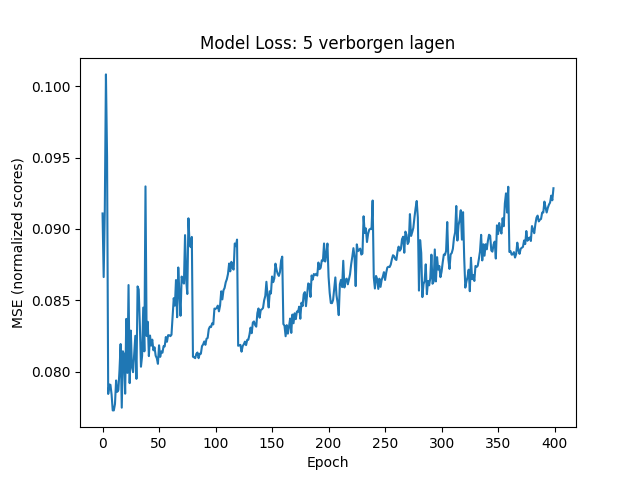
\includegraphics[width=1\linewidth]{fig/chapt5/inleiding/mlp5_2023-05-19_13h32__EPOCHS=400_LOSS=0.0929_LR=0.01.png}
        \caption{SGD, learning rate = $0.01$}
        \label{fig:chapt5_inleiding_sgd_suckt_1}
    \end{subfigure}
    \begin{subfigure}{.5\textwidth}
        \centering
        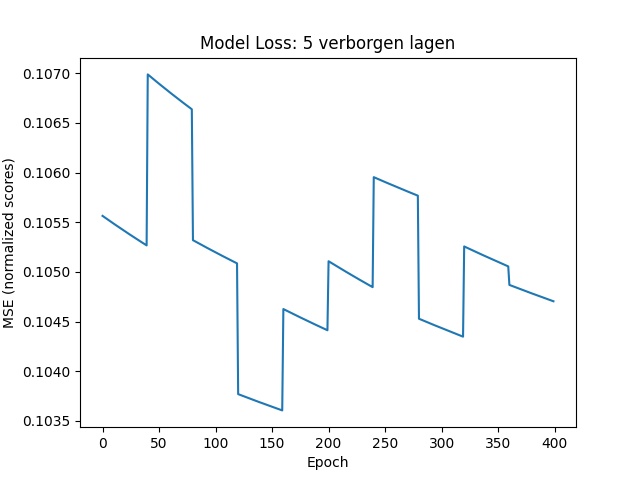
\includegraphics[width=1\linewidth]{fig/chapt5/inleiding/mlp5_2023-05-19_13h32__EPOCHS=400_LOSS=0.105_LR=0.0001.png}
        \caption{SGD, learning rate = $0.0001$}
        \label{fig:chapt5_inleiding_sgd_suckt_2}
    \end{subfigure}
    \caption{Neurale netwerken getraind met dezelfde inputdata}
    \label{fig:chapt5_inleiding_sgd_suckt_combined}
\end{figure}


\section{NLP-profielen}
\label{sub:chapt5_nlp_resultaten}
De eerste stap is het valideren van gebruikers- en restaurantprofielen gegenereerd door verschillende combinaties van parameters en NLP-modellen. We bekijken welke combinatie het neuraal netwerk het beste in staat stelt om accurate voorspellingen te maken. We toetsen steeds onze meetresultaten met een tweezijdige ongepaarde t-toets, om te bepalen of we statistisch significante verschillen waarnemen. Dit betekent dat bij elke conclusie er ofwel een significant verschil waargenomen werd, ofwel geen verschil aangetoond kon worden.\newline
Vervolgens analyseren we of de gebruikte BERTopic-modellen overeenkomen met de resultaten van de clusteringsmetrieken uit \autoref{sub:chapt4_eval_clustering}. 


\subsection{Parameters voor gebruikers- en restaurantprofielen}
\label{sub:chapt5_vergelijking_profielen}
Het eerste experiment bestaat uit de prestaties vergelijken van een offline BERTopic model tegenover zijn online variant. Hiervoor gebruiken we voor beide modellen dezelfde parameterconfiguratie. Het enige verschil is dat het offline model op 2\% van de data getraind is, terwijl de online variant de volledige dataset gebruikt.

% offline vs ONLINE
\mijnfiguur[H]{width=10cm}{fig/chapt5/NLP/nlp_comparison_offline.png}{Vergelijken van profielen zonder sentiment analysis gegenereerd door een offline model van 50 topics tegenover online modellen van 50 en 400 topics.}{fig:chapt5_nlp_offline_vs_online}

Uit \autoref{fig:chapt5_nlp_offline_vs_online} kunnen we concluderen dat het gebruik van een online model een significante verbetering geeft. Daarom gaan we vanaf hier enkel de online modellen met elkaar vergelijken. Een andere onderzoeksparameter is het gebruik van sentiment analysis. Hierbij onderzoeken we het effect van sentiment analysis op gebruikers- en restaurantprofielen. Verder analyseren we ook of eenzelfde trend tussen een gebruikersprofiel en een restaurantprofiel zichtbaar is.

% USER - RESTAURANT (sentiment) \label{fig:chapt5_nlp_sentiment_comparison}
% A: vergelijk (kolom 2 VS 6) \label{fig:chapt5_nlp_sentiment_user}   
% B: vergelijk (rij 3 VS 6) \label{fig:chapt5_nlp_sentiment_restaurant}
\begin{figure}[H]

        \centering
        \parbox[b]{0.6\textwidth}{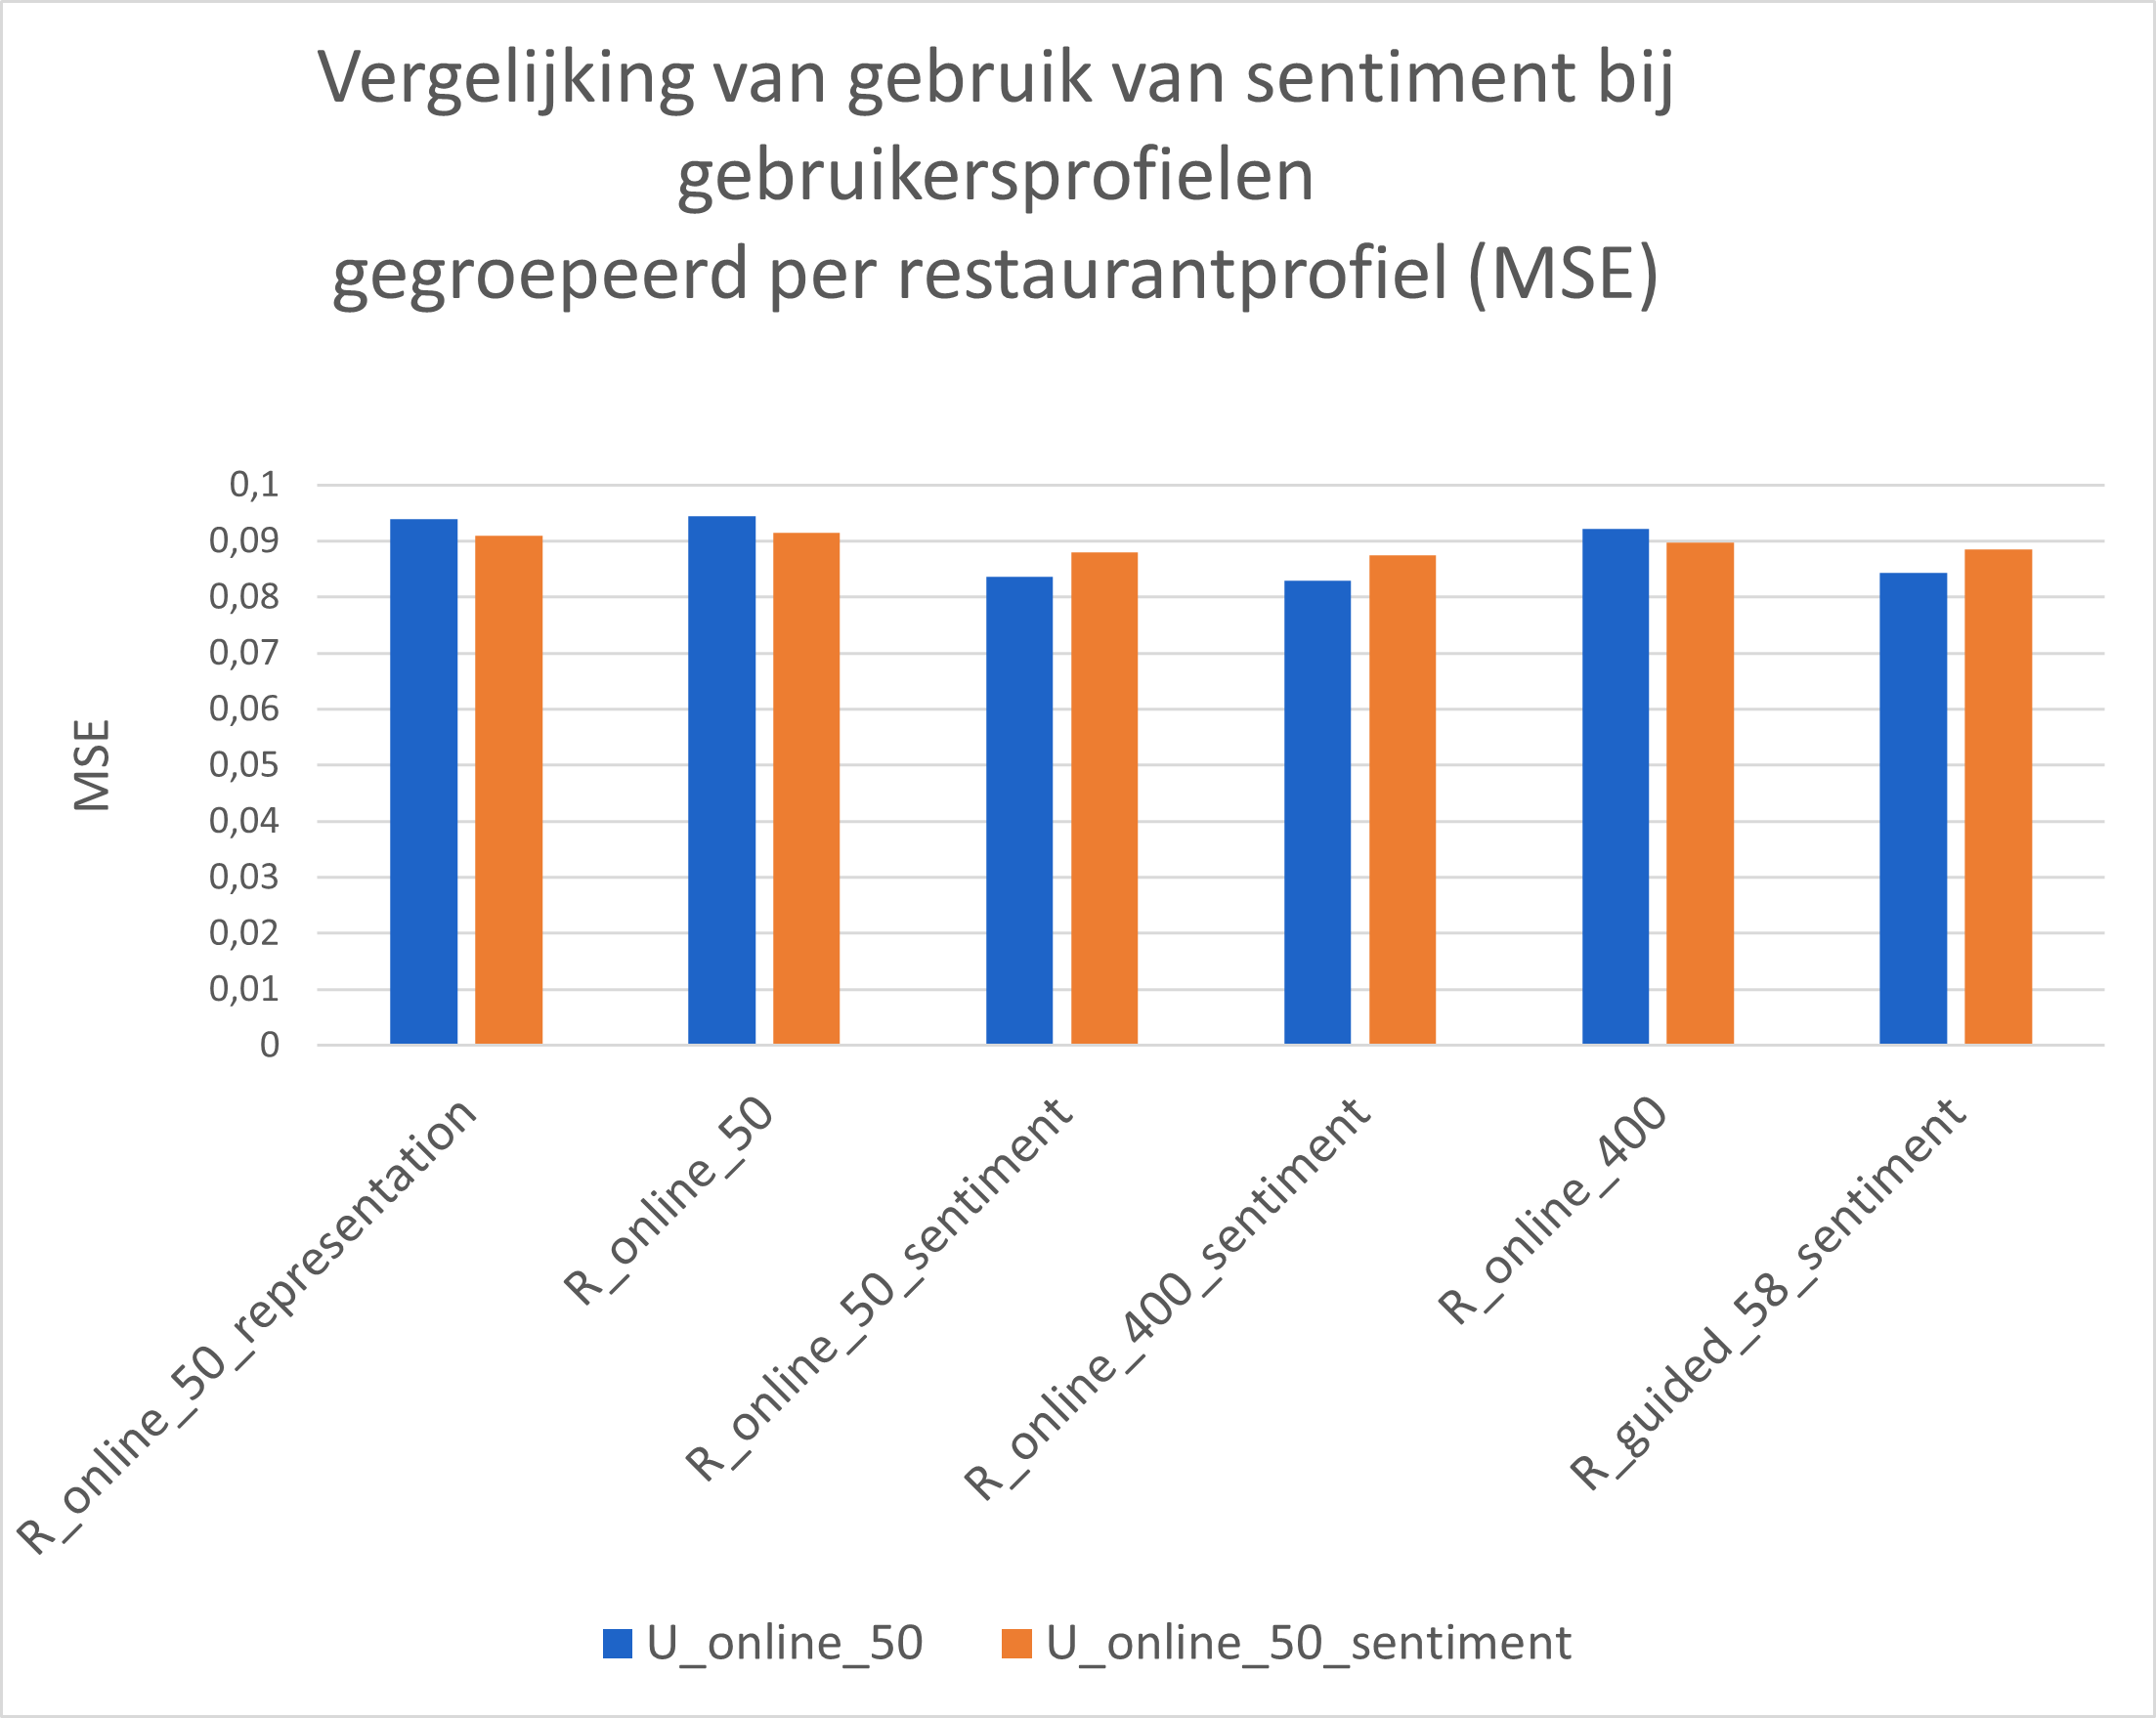
\includegraphics[width=\linewidth]{fig/chapt5/NLP/nlp_comparison_sentiment_gebruiker.png}}\quad
        \parbox[b]{0.37\textwidth}{
        \subcaption{Gebruikersprofiel zonder sentiment (blauw) en gebruikersprofiel met sentiment (oranje) vergeleken met verschillende restaurantprofielen op basis van MSE.}\label{fig:chapt5_nlp_sentiment_user}}
        \\[.5cm]

        \centering
        \parbox[b]{0.6\textwidth}{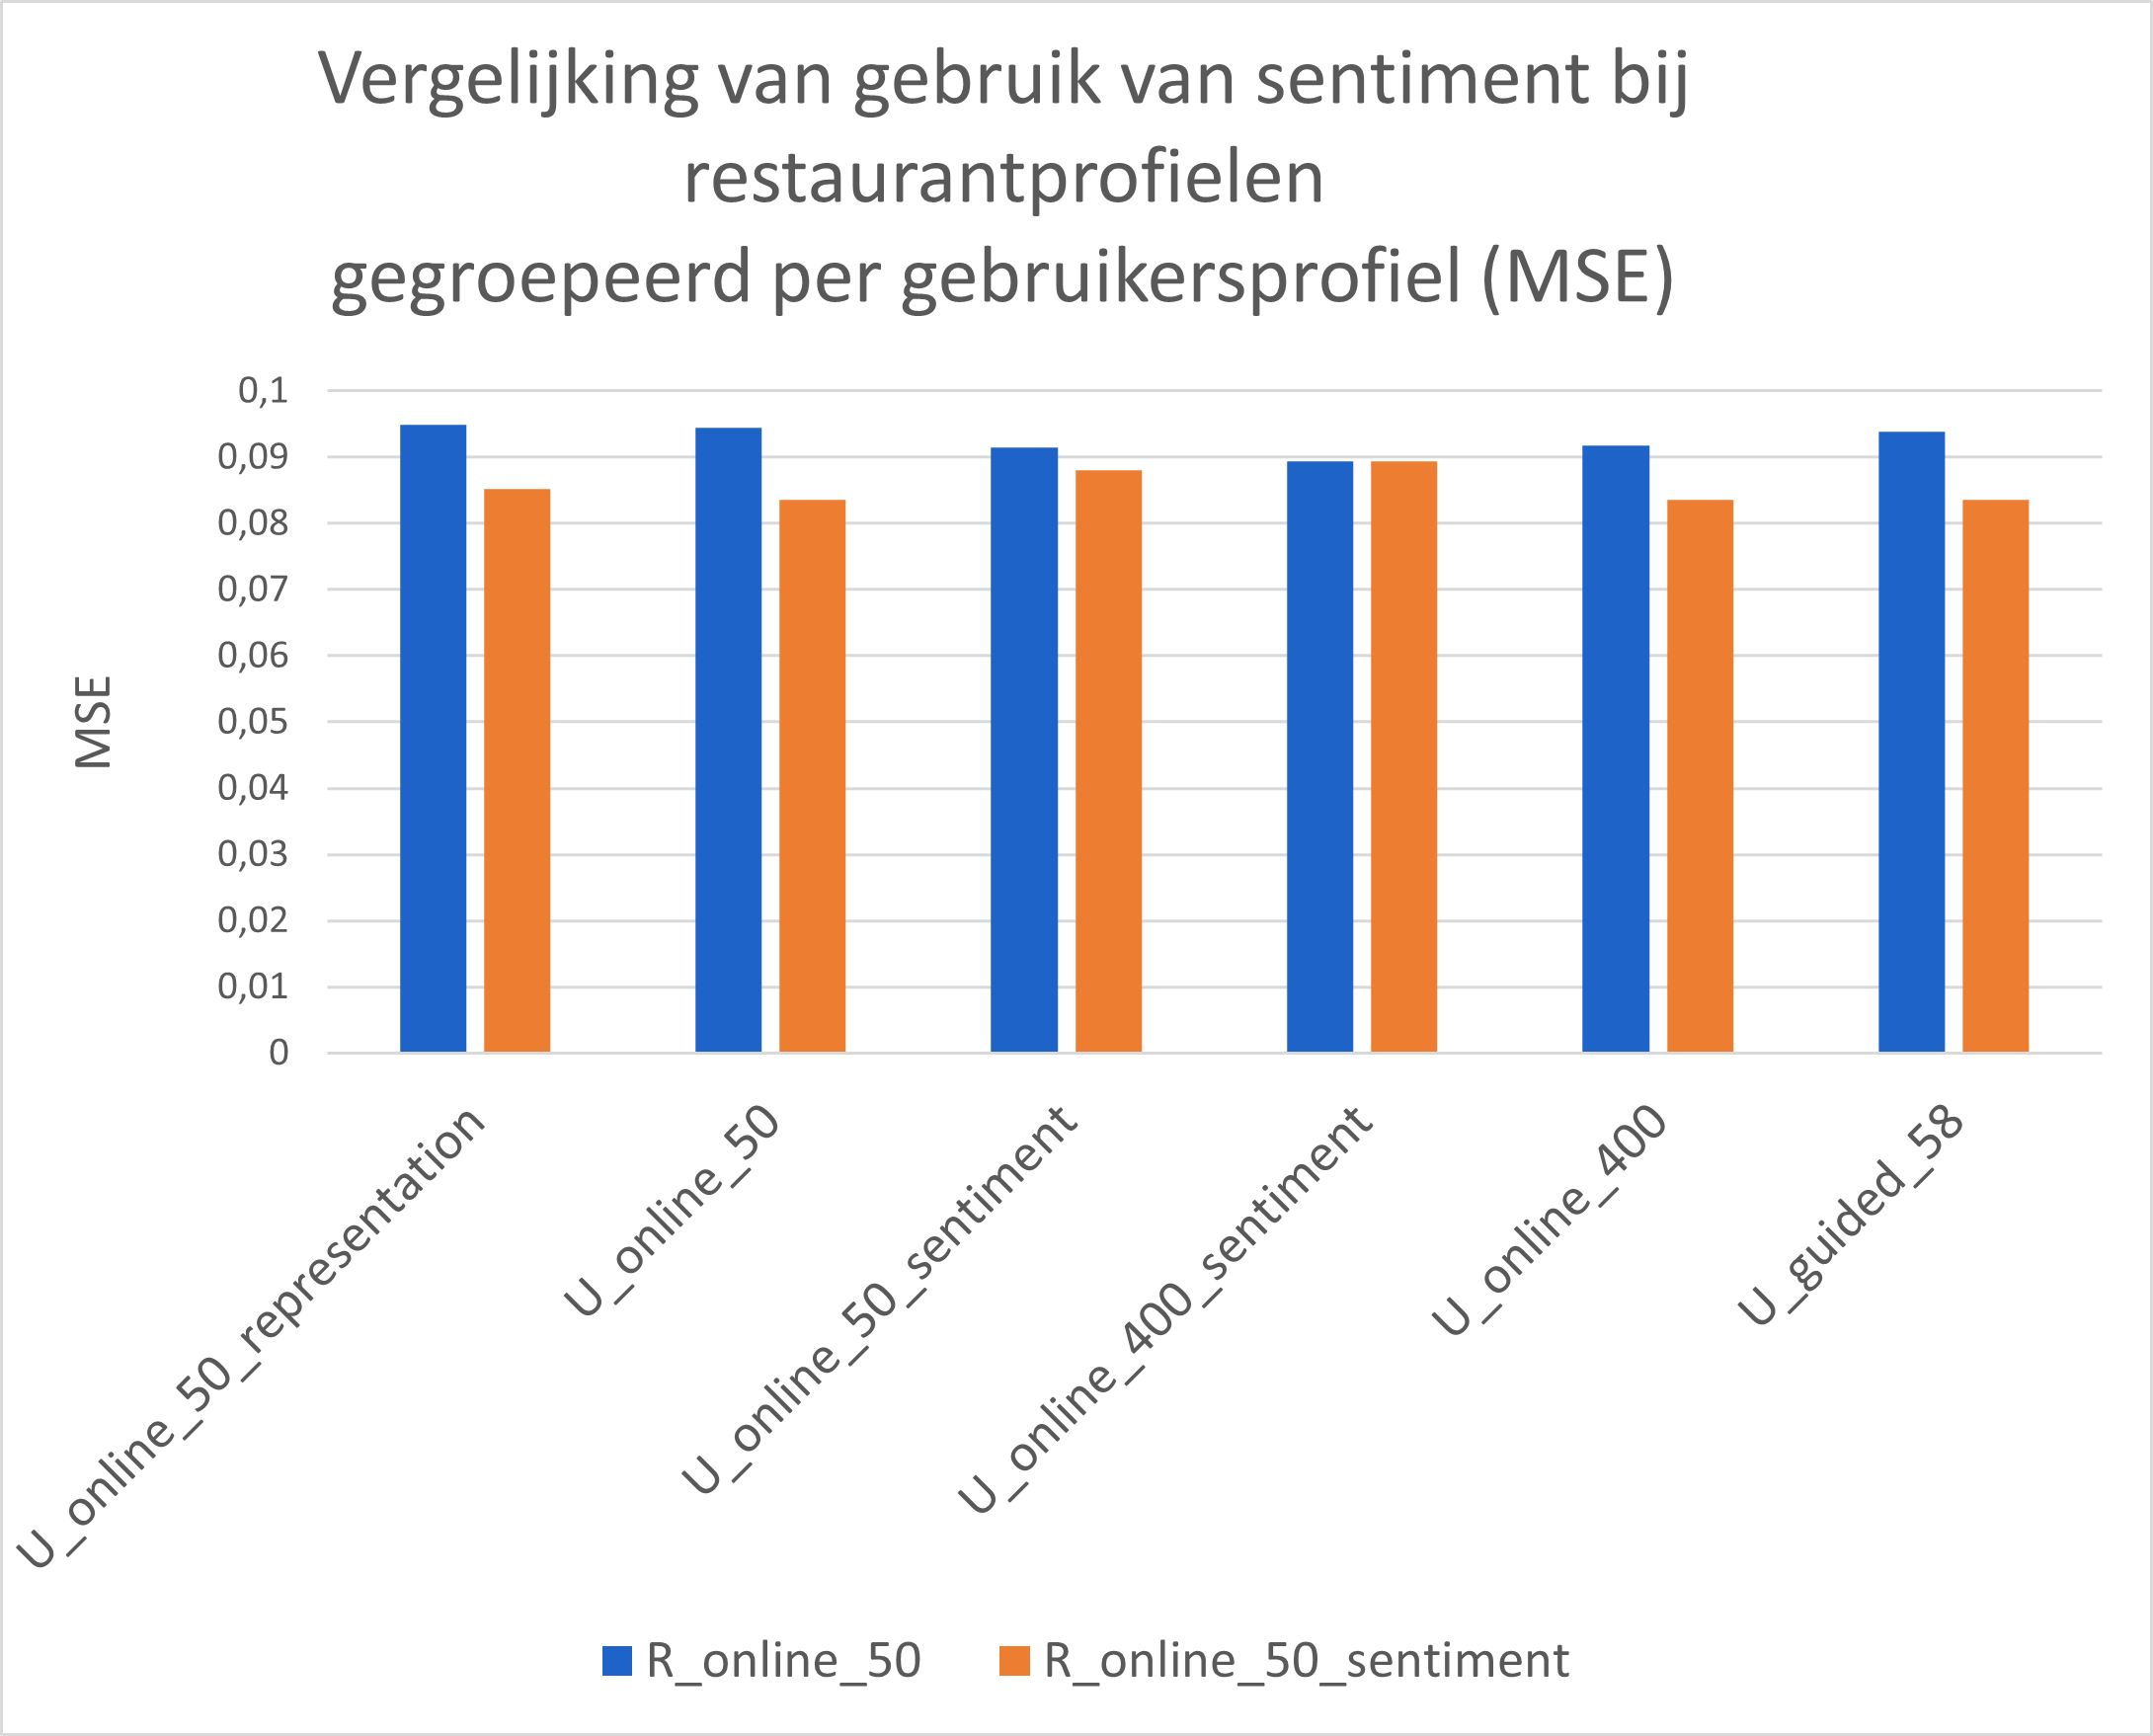
\includegraphics[width=\linewidth]{fig/chapt5/NLP/nlp_comparison_sentiment_restaurant.png}}\quad
        \parbox[b]{0.37\textwidth}{
        \subcaption{Restaurantprofiel zonder sentiment (blauw) en restaurantprofiel met sentiment (oranje) vergeleken met verschillende gebruikersprofielen op basis van MSE.}\label{fig:chapt5_nlp_sentiment_restaurant}}
        \\[.5cm]

        \caption{Analyse van de toegevoegde waarde van sentiment analysis bij het genereren van gebruikers- en restaurantprofielen.}
        \label{fig:chapt5_nlp_sentiment_comparison}
\end{figure}

Uit de grafieken afgebeeld in \autoref{fig:chapt5_nlp_sentiment_comparison} kunnen we enkele zaken besluiten: het toevoegen van sentiment analysis bij gebruikersprofielen resulteert in een kleine daling in MSE indien de restaurantprofielen geen sentiment gebruiken. Indien een restaurantprofiel wel sentiment gebruikt, presteert een gebruikersprofiel zonder sentiment beter zoals in \autoref{fig:chapt5_nlp_sentiment_user}. Analoog kunnen we de vergelijking maken voor restaurantprofielen: hierbij zien we een gelijkaardig effect. Aan de hand van \autoref{fig:chapt5_nlp_sentiment_restaurant} nemen we waar dat er een significante daling is in MSE bij het gebruik van sentiment bij restaurantprofielen in combinatie met gebruikersprofielen zonder sentiment. Indien een gebruikersprofiel toch sentiment toevoegt, is deze stijging nog steeds significant, maar is het verschil in performantie merkbaar kleiner.

Voor de beste prestaties gaan we enkel sentiment gebruiken bij een restaurantprofiel. Dit kunnen we afleiden uit beide grafieken door de combinatie van profielen met de laagste MSE te nemen. De hypothese uit \autoref{sub:chapt4_users_vs_restaurants} waarbij we geen sentiment analysis gaan toepassen op de gebruikersprofielen maar wel op de restaurantprofielen is dus geldig. \\


% A: vergelijk (kolom 2 VS 1) telkens approx vs geen approx => analoog: vrij gelijkaardig voor user      \label{fig:chapt5_nlp_approx_vs_topics_users}
% B: vergelijk (rij 2 VS 1) telkens approx vs geen approx => vrij gelijkaardig voor restaurants          \label{fig:chapt5_nlp_approx_vs_topics_restaurant}
\begin{figure}[H]

        \centering
        \parbox[b]{0.6\textwidth}{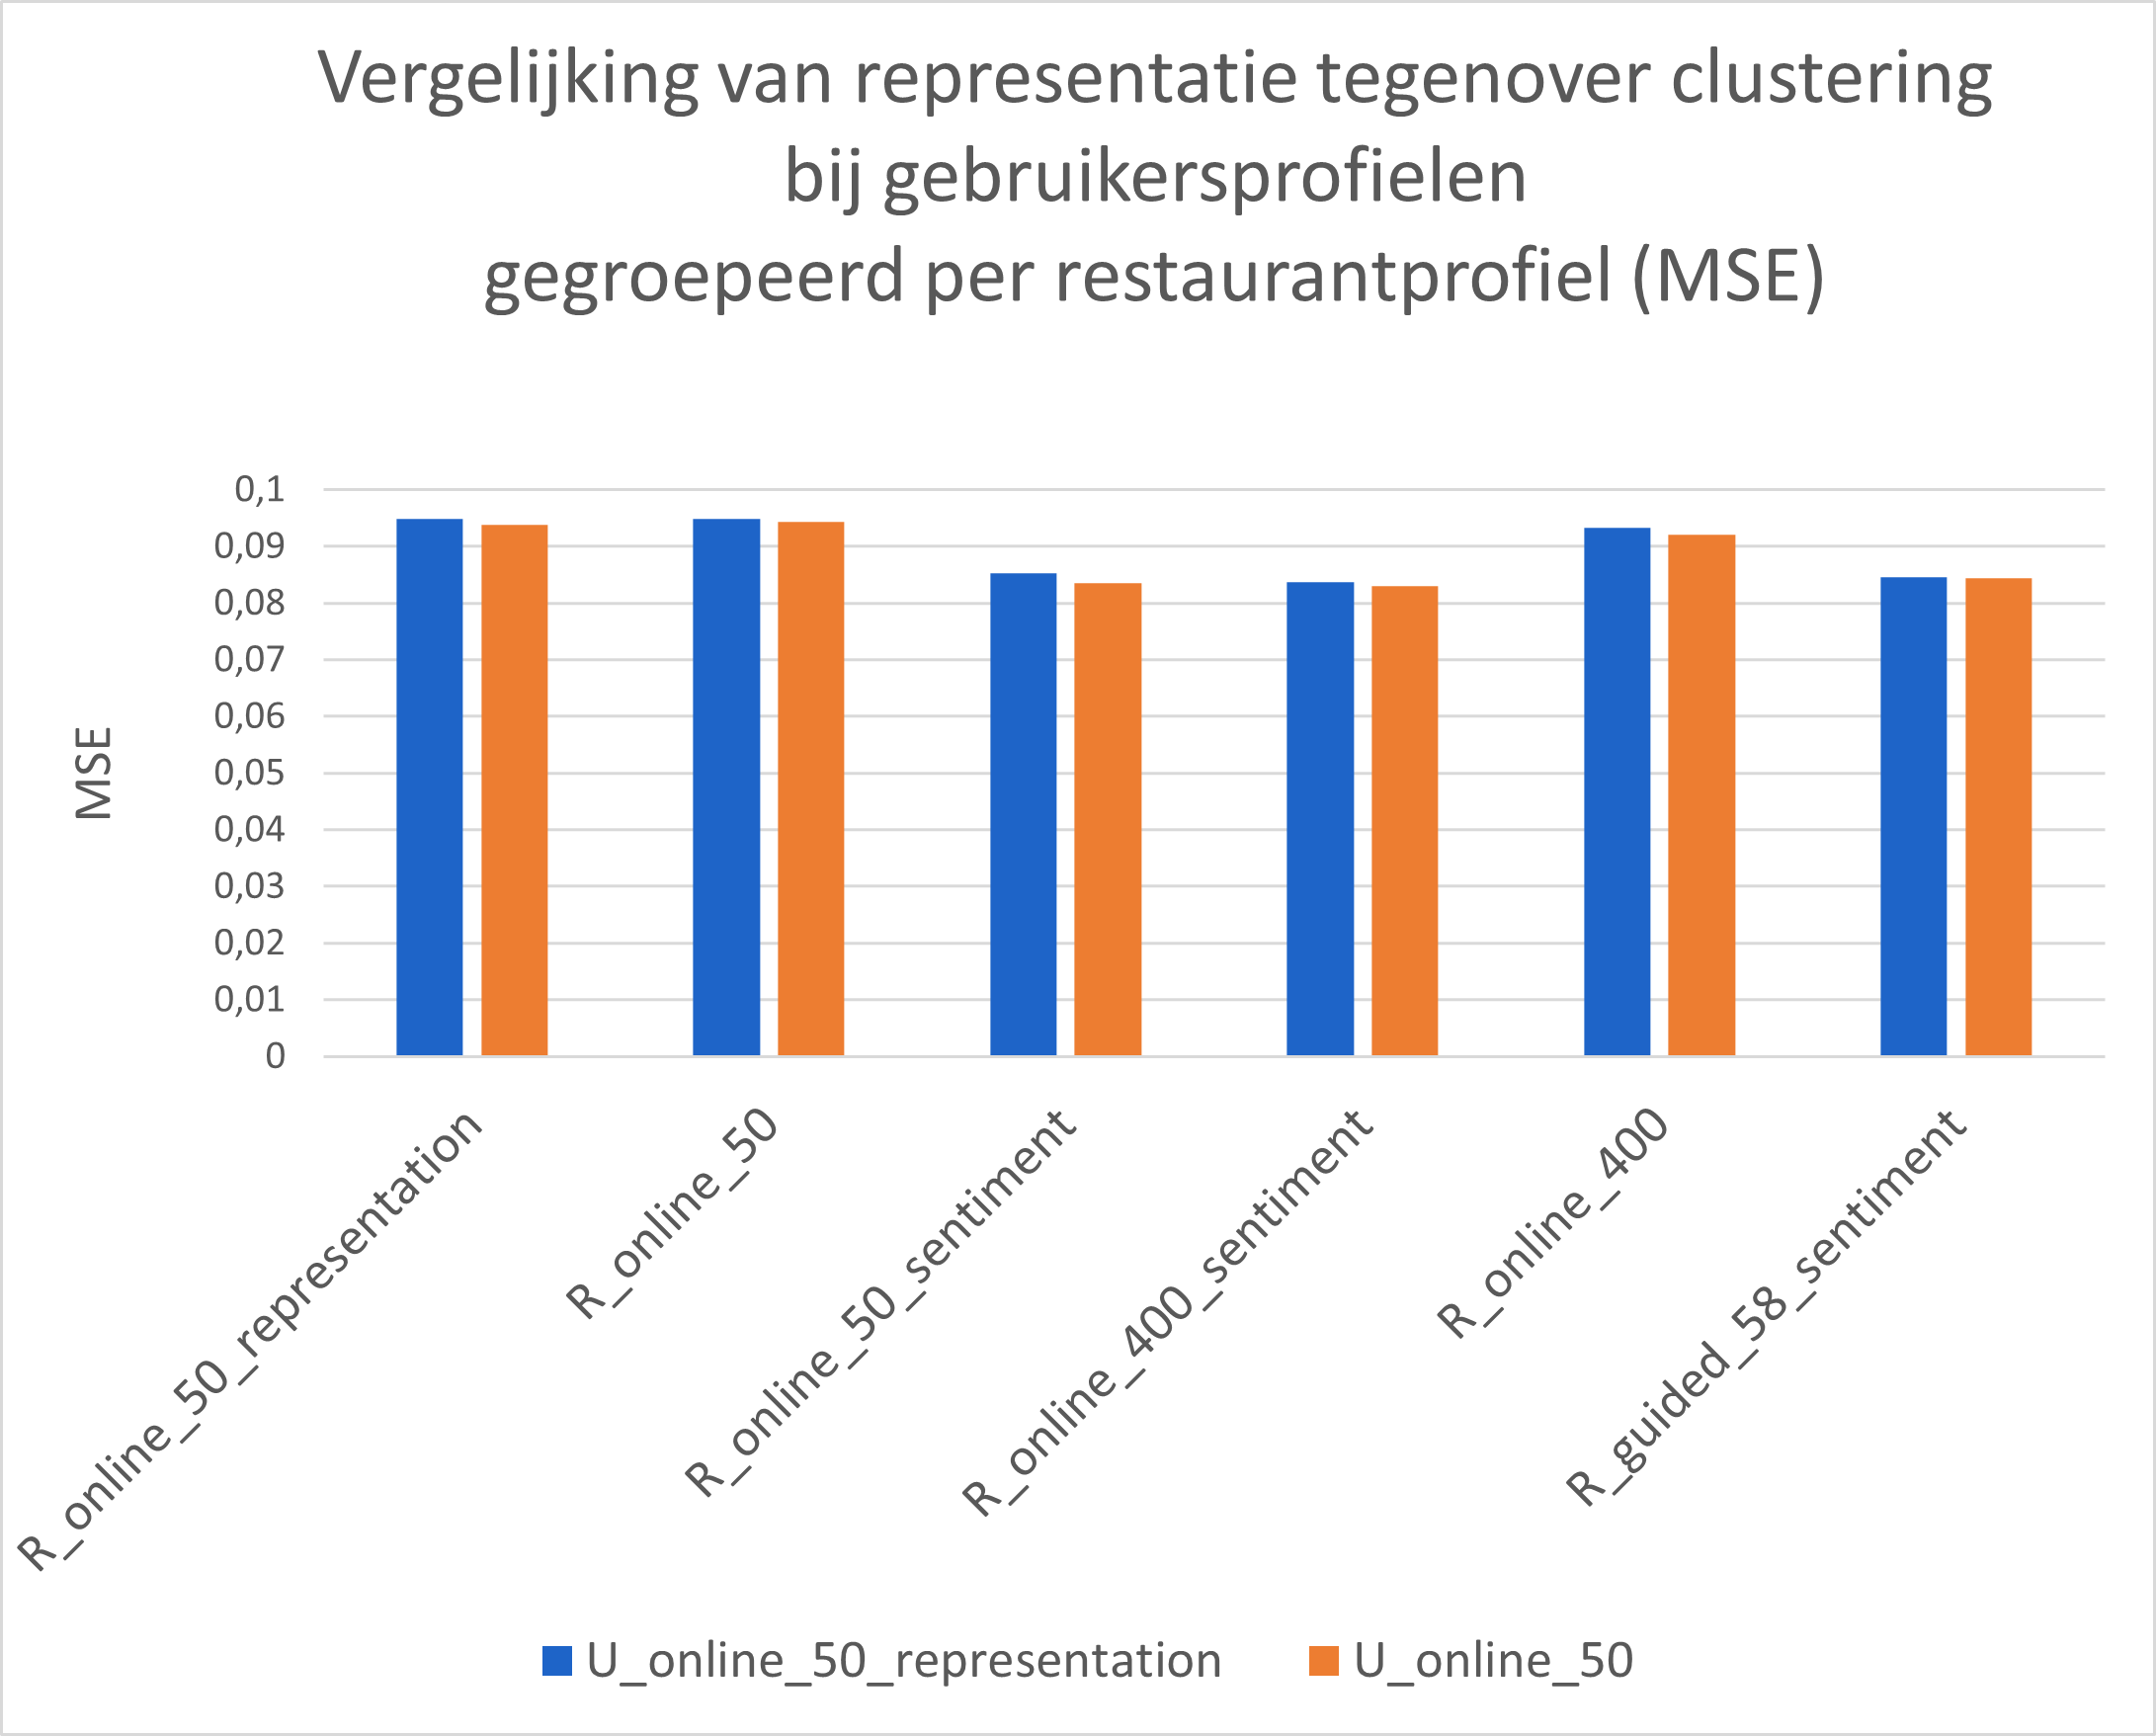
\includegraphics[width=\linewidth]{fig/chapt5/NLP/nlp_comparison_approx_gebruiker.png}}\quad
        \parbox[b]{0.37\textwidth}{
        \subcaption{Gebruikersprofiel op basis van representatie (blauw) en gebruikersprofiel op basis van clustering (oranje) vergeleken met verschillende restaurantprofielen op basis van MSE.}\label{fig:chapt5_nlp_approx_vs_topics_users}}
        \\[.5cm]

        \centering
        \parbox[b]{0.6\textwidth}{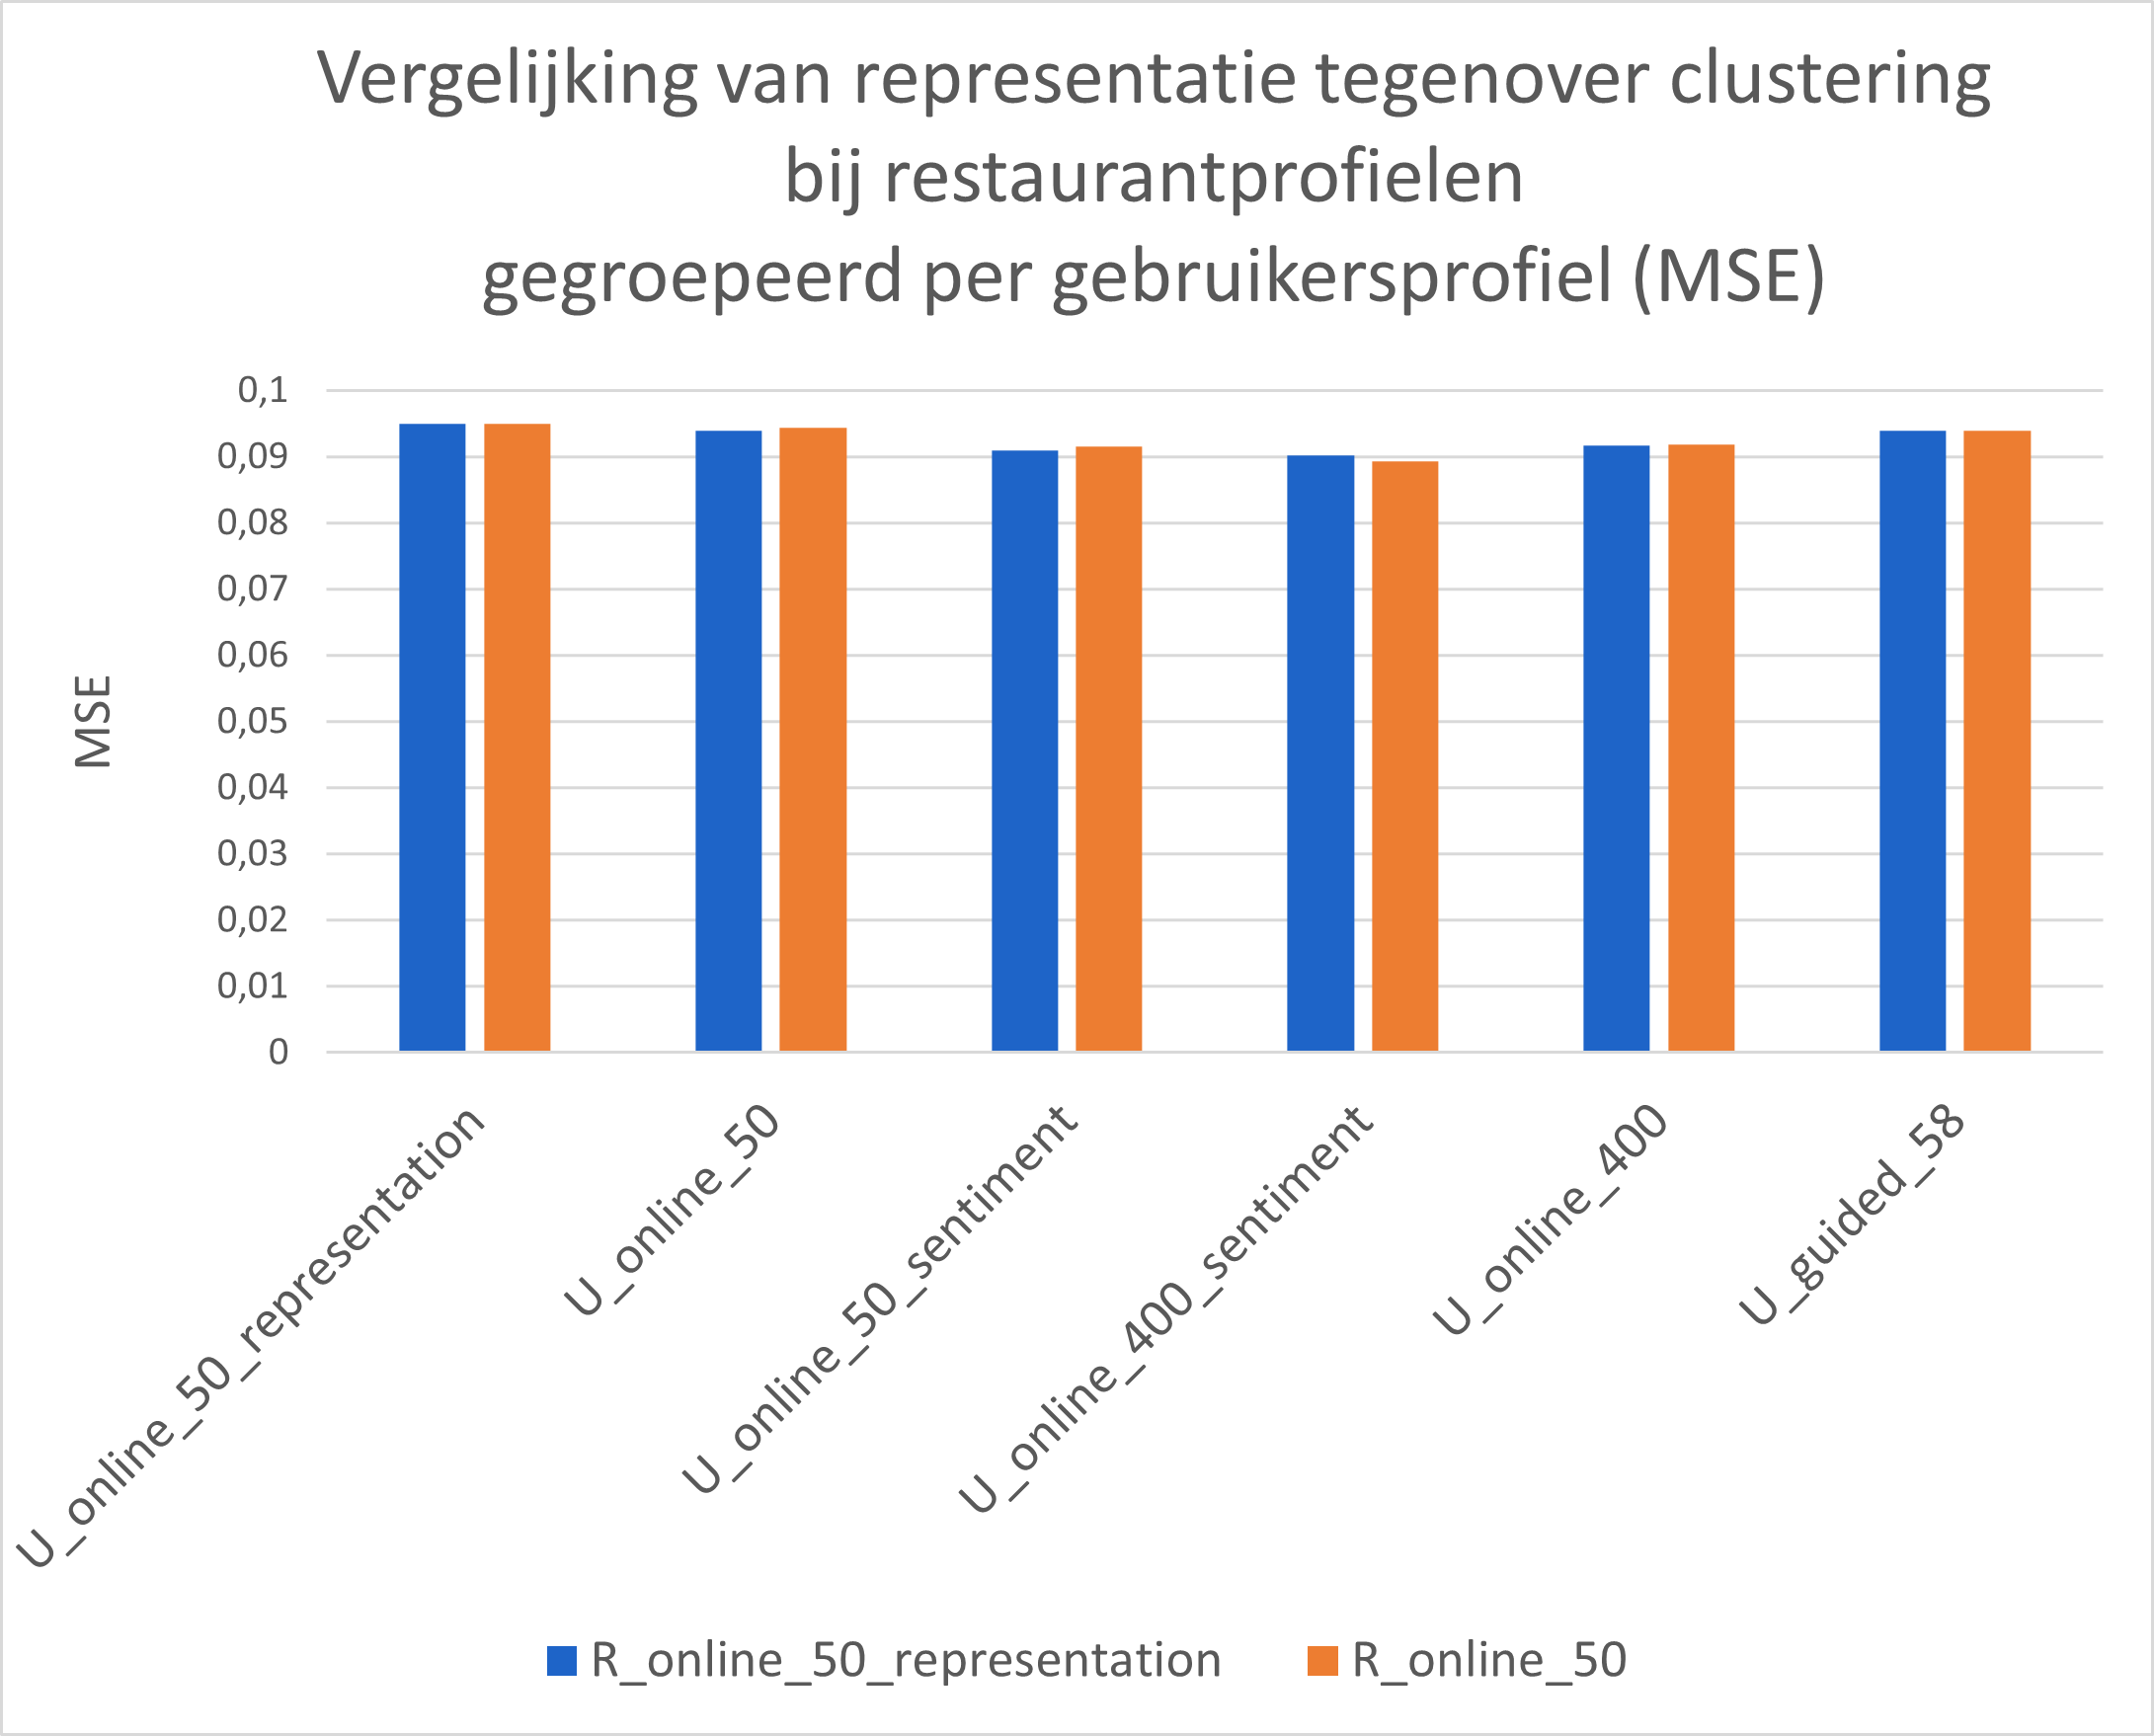
\includegraphics[width=\linewidth]{fig/chapt5/NLP/nlp_comparison_approx_restaurant.png}}\quad
        \parbox[b]{0.37\textwidth}{
        \subcaption{Restaurantprofiel op basis van representatie (blauw) en restaurantprofiel op basis van clustering (oranje) vergeleken met verschillende gebruikersprofielen op basis van MSE.}\label{fig:chapt5_nlp_approx_vs_topics_restaurant}}
        \\[.5cm]

        \caption{Analyse van de performantie van profielen op basis van clustering tegenover profielen op basis van representatie.}
        \label{fig:chapt5_nlp_approx_vs_topics}
\end{figure}

In \autoref{fig:chapt5_nlp_approx_vs_topics} vergelijken we de profielen op basis van clustering tegenover profielen op basis van representaties, zoals beschreven in \autoref{sec:chapt4_nlp_profielen}. Analoog aan sentiment analysis maken we een onderscheid tussen gebruikers- en restaurantprofielen. In \autoref{fig:chapt5_nlp_approx_vs_topics_users} vergelijken we een gebruikersprofiel op basis van clustering tegenover gebruikersprofiel op basis van representatie in combinatie met verschillende restaurantprofielen. We concluderen dat de resultaten heel gelijkaardig zijn aan elkaar. Analoog doen we dit voor restaurantprofielen, zoals weergegeven in \autoref{fig:chapt5_nlp_approx_vs_topics_restaurant}. Net zoals de gebruikersprofielen nemen we geen significante verschillen waar. 

Vervolgens vergelijken we een online model van 50 topics met een guided variant van 48 voorgedefinieerde topics en 10 extra topics. Het doel van extra topics is om de overige niet-relevant informatie op te vangen. In \autoref{fig:chapt5_nlp_guided} vergelijken we beide als gebruikersprofiel in combinatie met andere restaurantprofielen en vice versa. \\

% guided vs online  \label{fig:chapt5_nlp_guided}
% A: vergelijk (kolom 2 VS 3) \label{fig:chapt5_nlp_guided_user}   
% B: vergelijk (rij 2 VS 3) \label{fig:chapt5_nlp_guided_restaurant}
\begin{figure}[H]

        \centering
        \parbox[b]{0.6\textwidth}{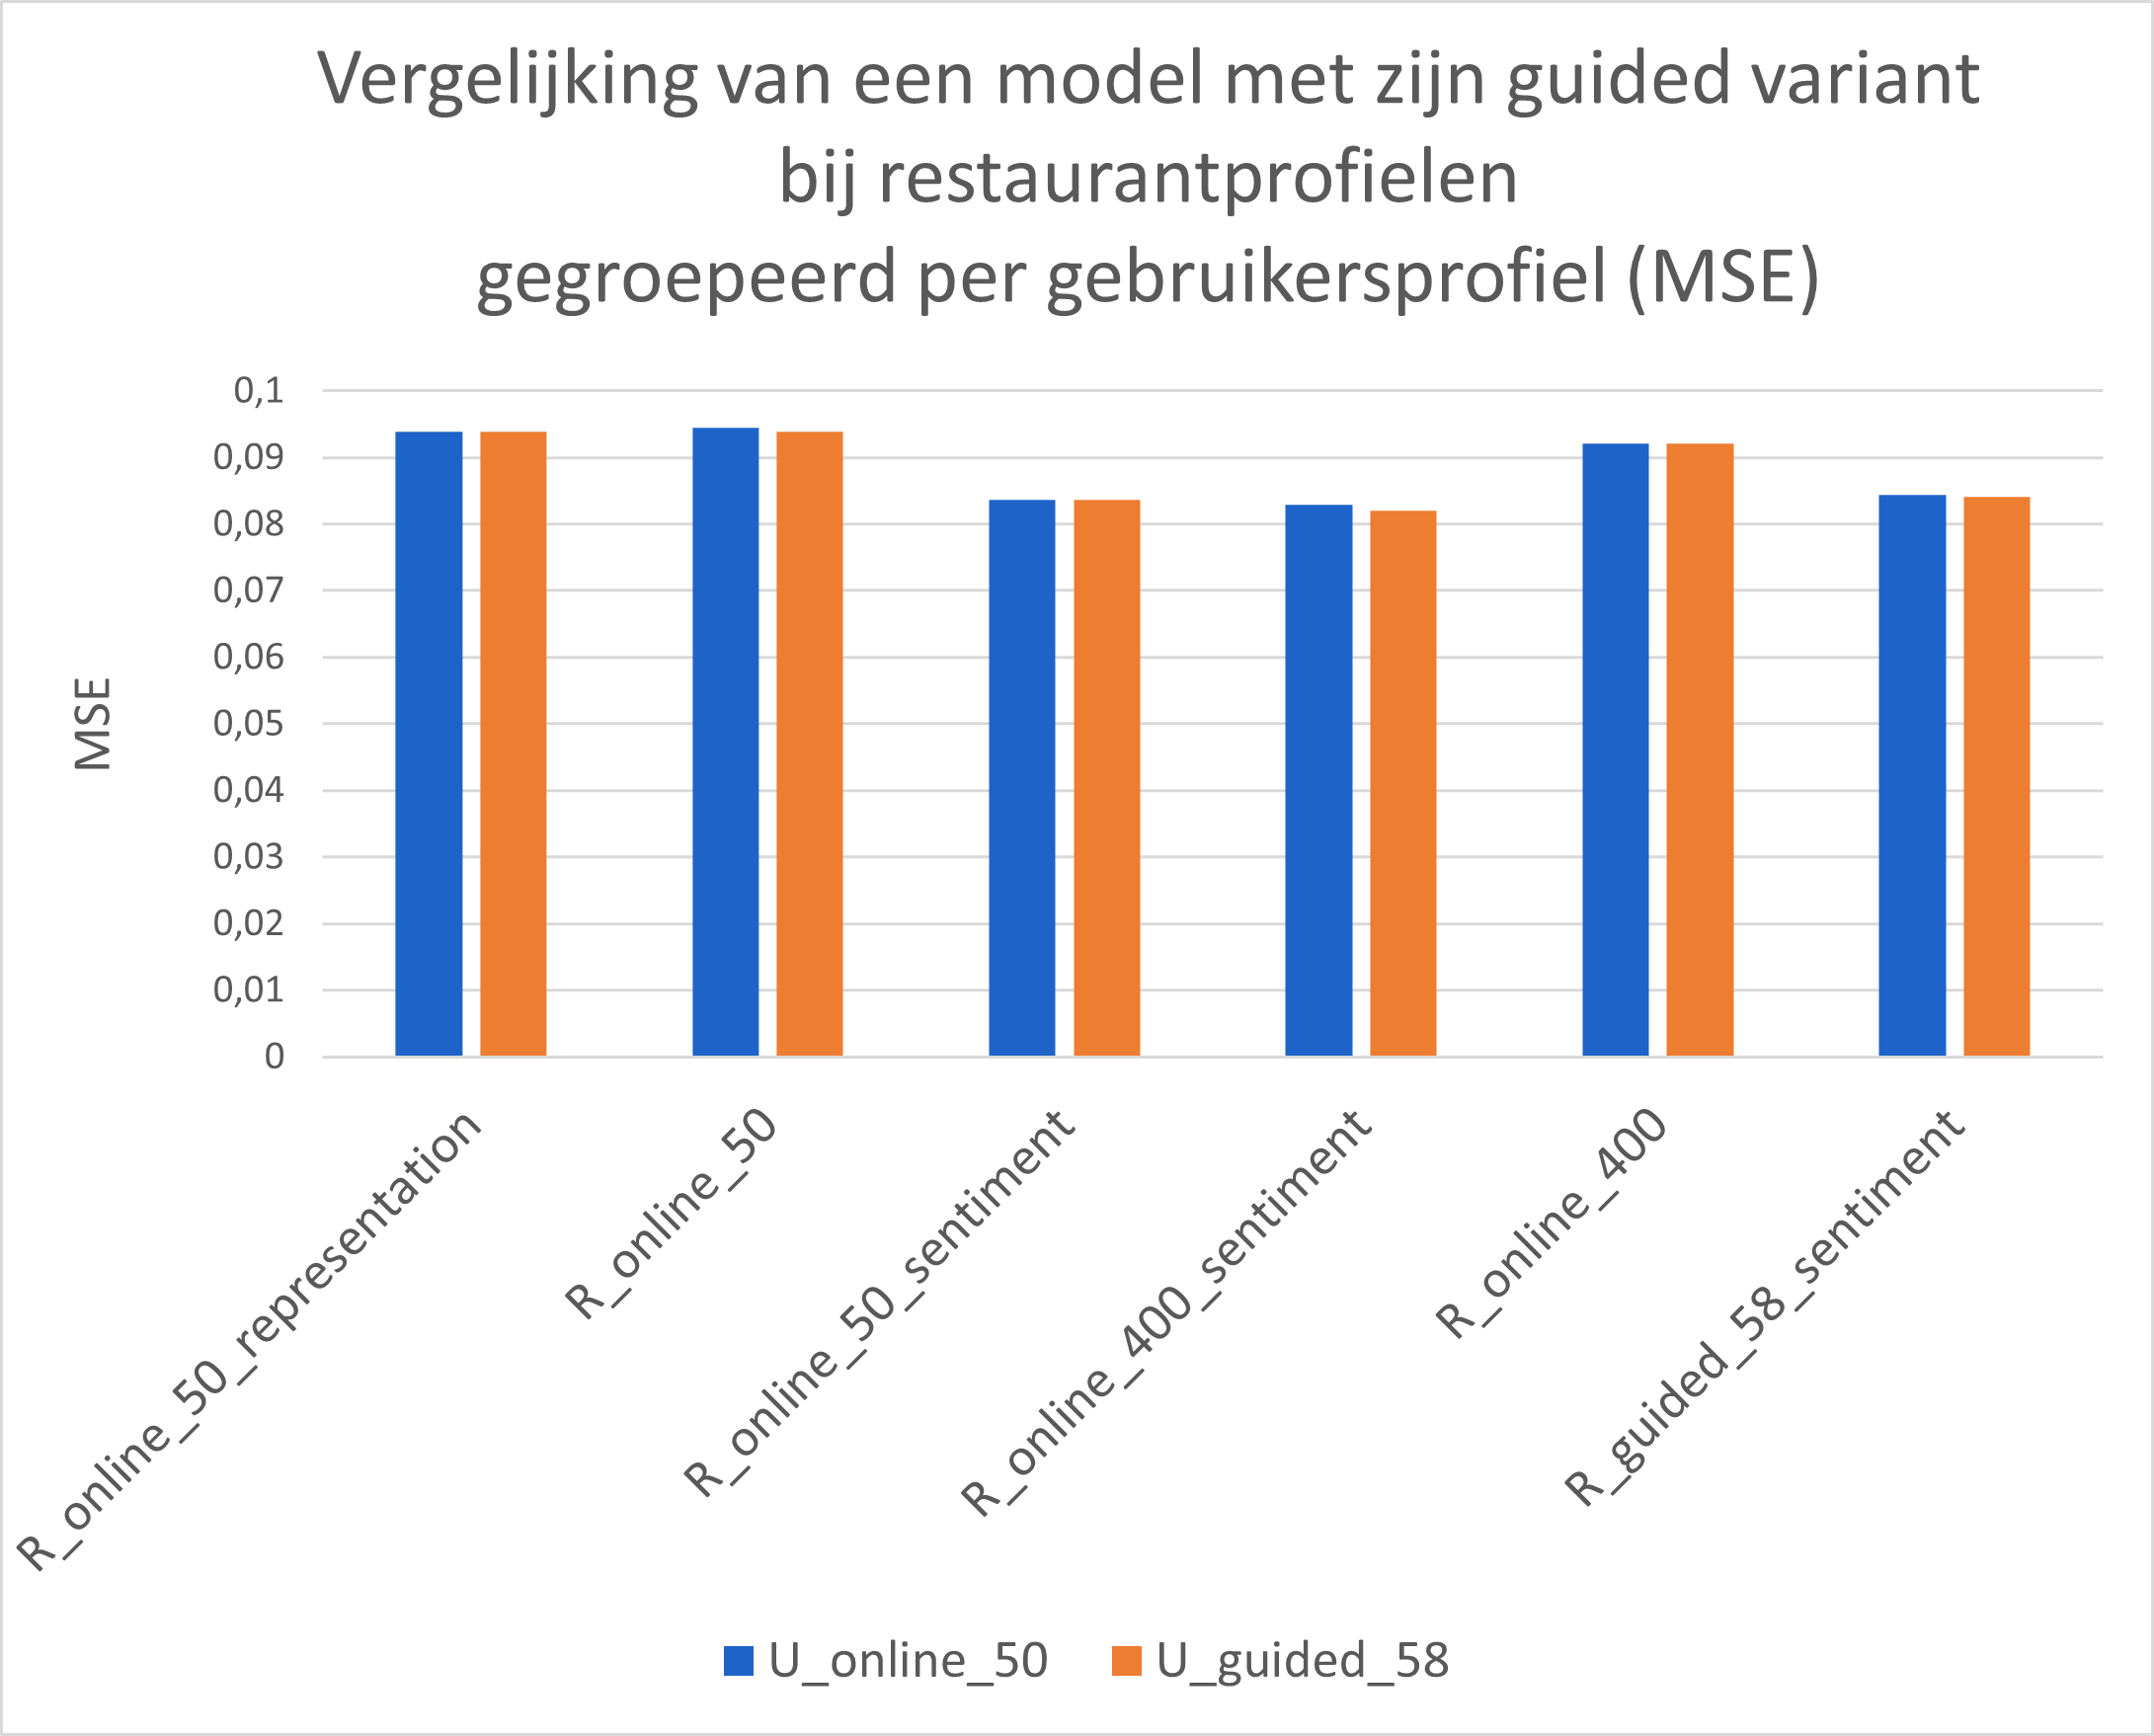
\includegraphics[width=\linewidth]{fig/chapt5/NLP/nlp_comparison_guided_gebruiker.png}}\quad
        \parbox[b]{0.37\textwidth}{
        \subcaption{Gebruikersprofiel van 50 topics (blauw) en gebruikersprofiel op basis van een guided model (oranje) vergeleken met verschillende restaurantprofielen op basis van MSE.}\label{fig:chapt5_nlp_guided_user}}
        \\[.5cm]

        \centering
        \parbox[b]{0.6\textwidth}{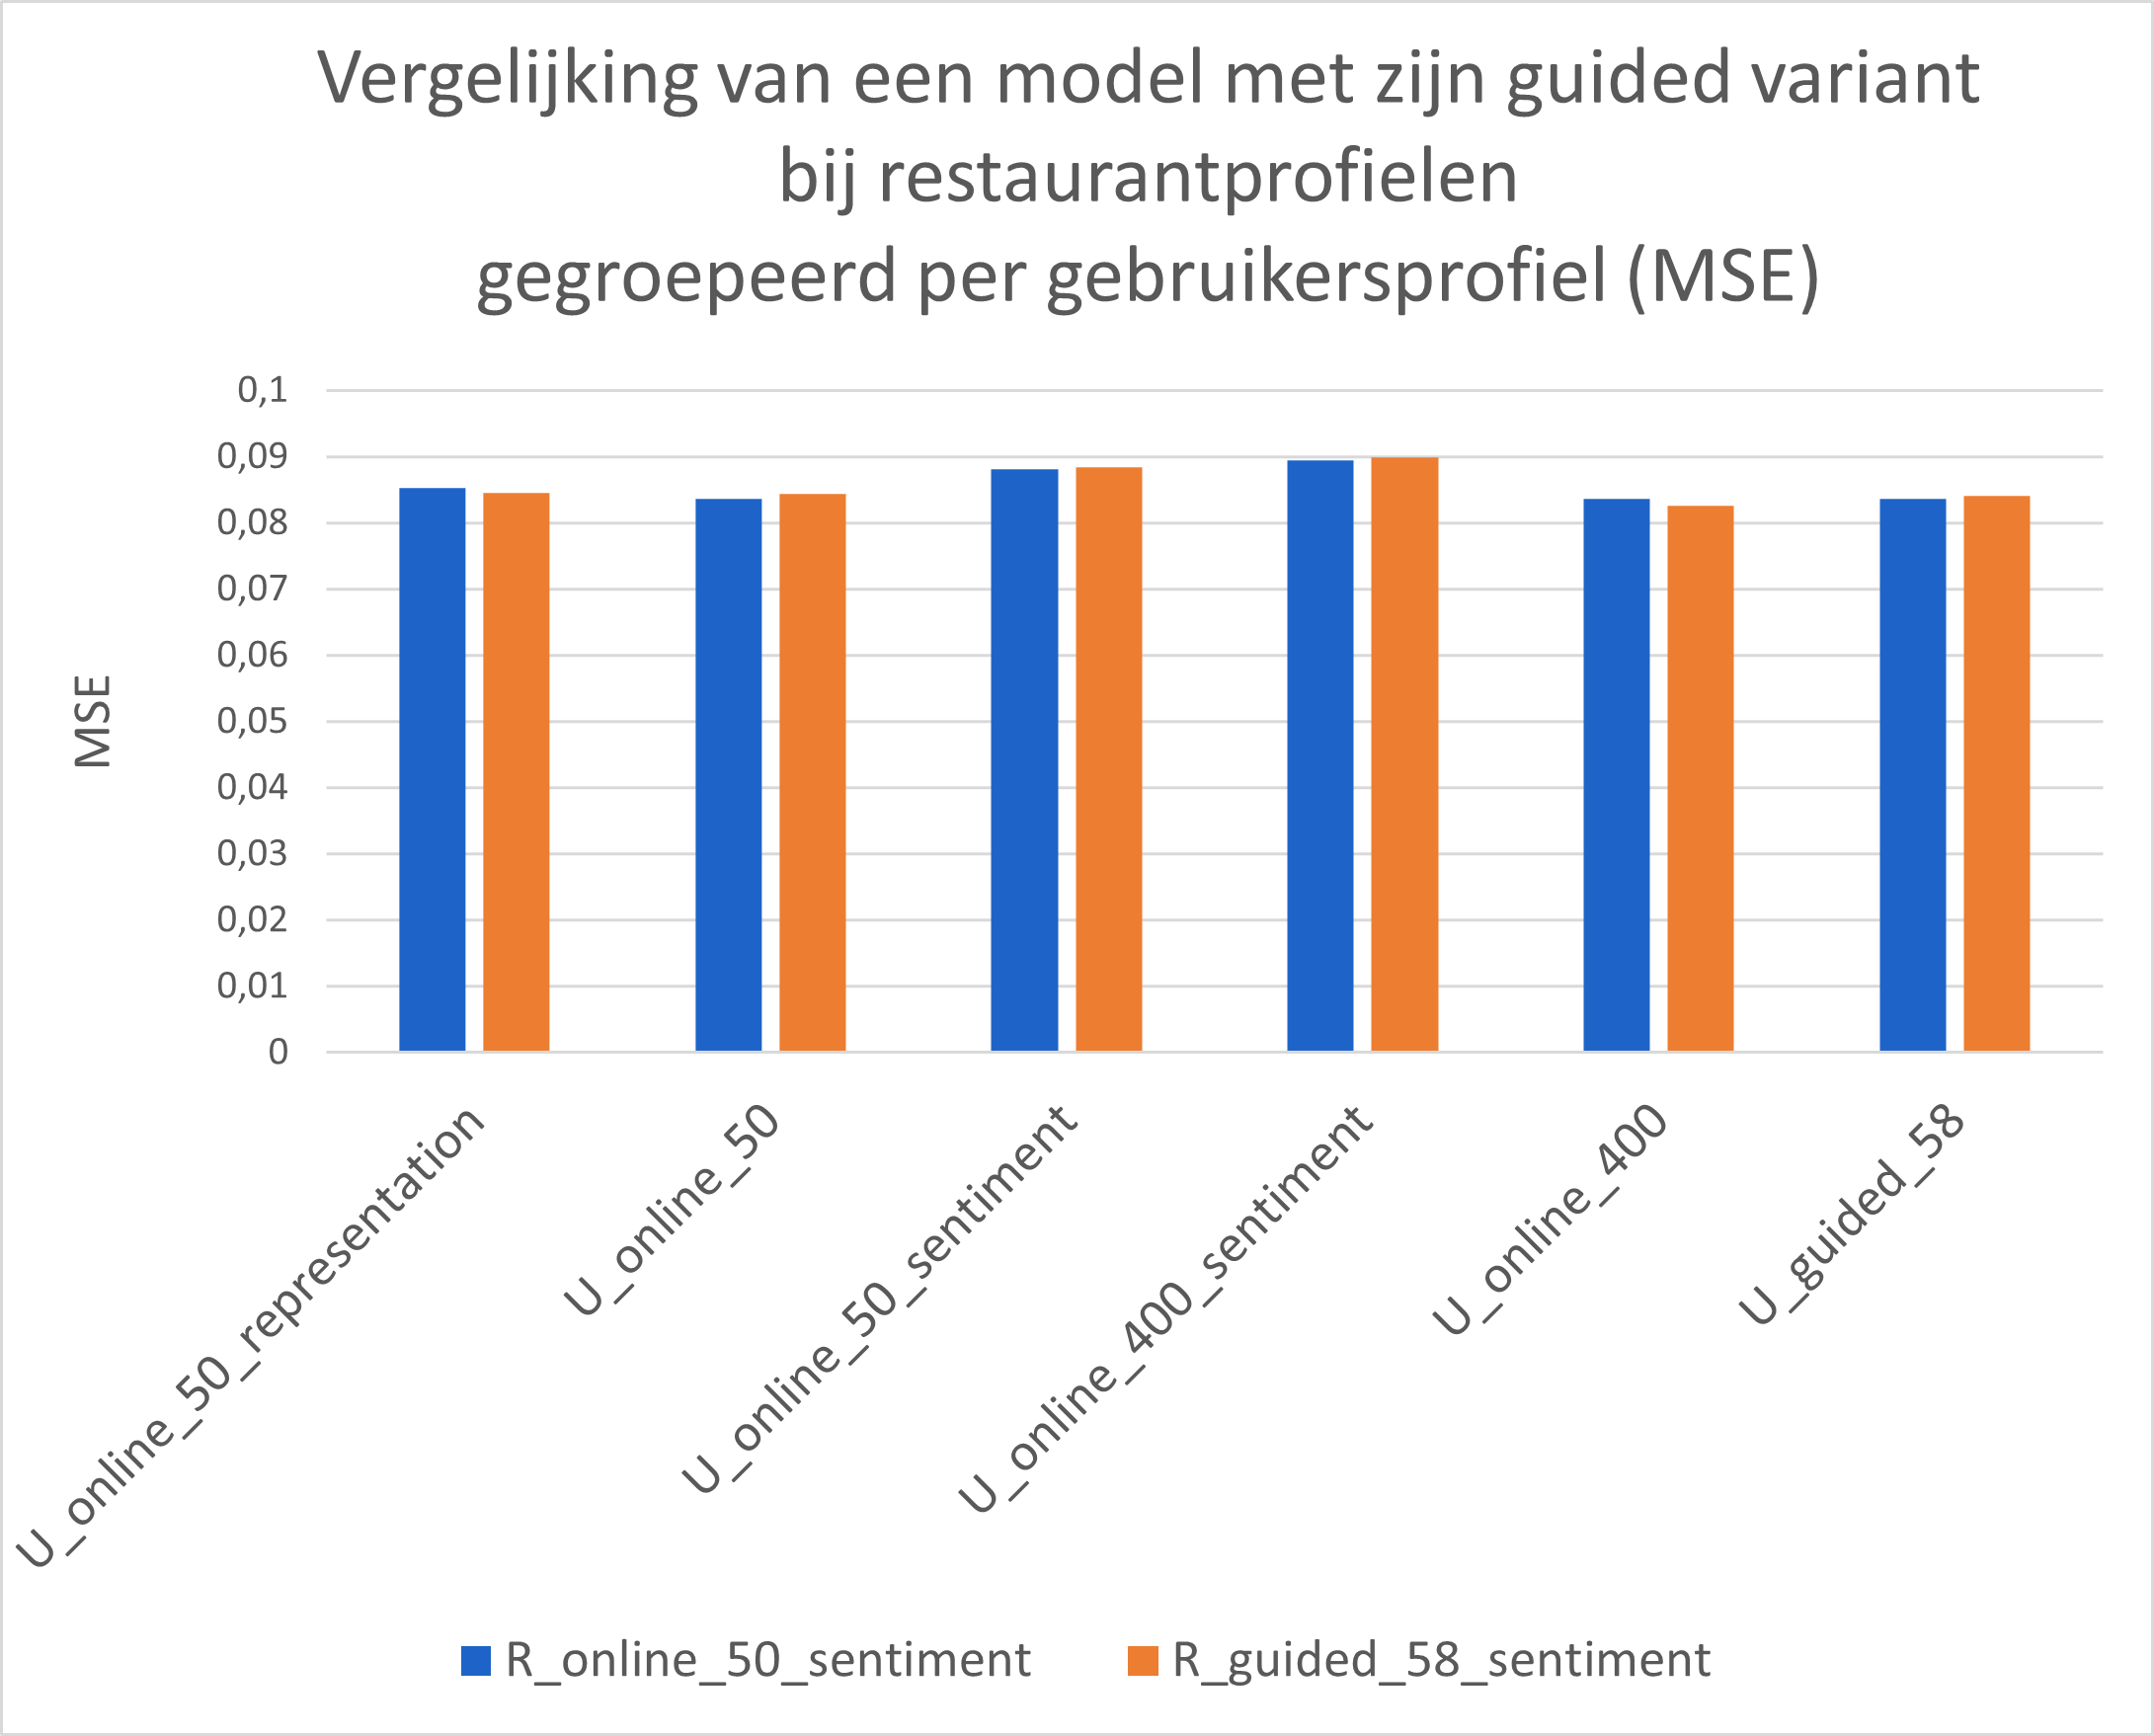
\includegraphics[width=\linewidth]{fig/chapt5/NLP/nlp_comparison_guided_restaurant.png}}\quad
        \parbox[b]{0.37\textwidth}{
        \subcaption{Restaurantprofiel van 50 topics (blauw) en restaurantprofiel op basis van een guided model (oranje) vergeleken met verschillende gebruikersprofielen op basis van MSE.}\label{fig:chapt5_nlp_guided_restaurant}}
        \\[.5cm]

        \caption{Analyse van de toegevoegde waarde van voorafgedefinieerde topics bij het genereren van gebruikers- en restaurantprofielen.}
        \label{fig:chapt5_nlp_guided}
\end{figure}

Zoals af te lezen op de grafieken in \autoref{fig:chapt5_nlp_guided}, is er geen significant verschil tussen een online model en zijn guided variant. Indien we manueel naar de topics kijken, vinden we weinig terug van de originele voorgedefinieerde topics. Een mogelijke verklaring is dat de hoeveelheid trainingsdata overheerst en deze topics zal overnemen. Een andere mogelijkheid is dat de voorgedefinieerde topics niet specifiek genoeg zijn waardoor er onvoldoende geconvergeerd wordt. \\

% aantal topics = lengte model = impact performance?  \label{fig:chapt5_nlp_size_model} 
% A: vergelijk (kolom 2 VS 5) \label{fig:chapt5_nlp_size_user}   
% B: vergelijk (rij 3 VS 4) \label{fig:chapt5_nlp_size_restaurant}
\begin{figure}[H]

        \centering
        \parbox[b]{0.6\textwidth}{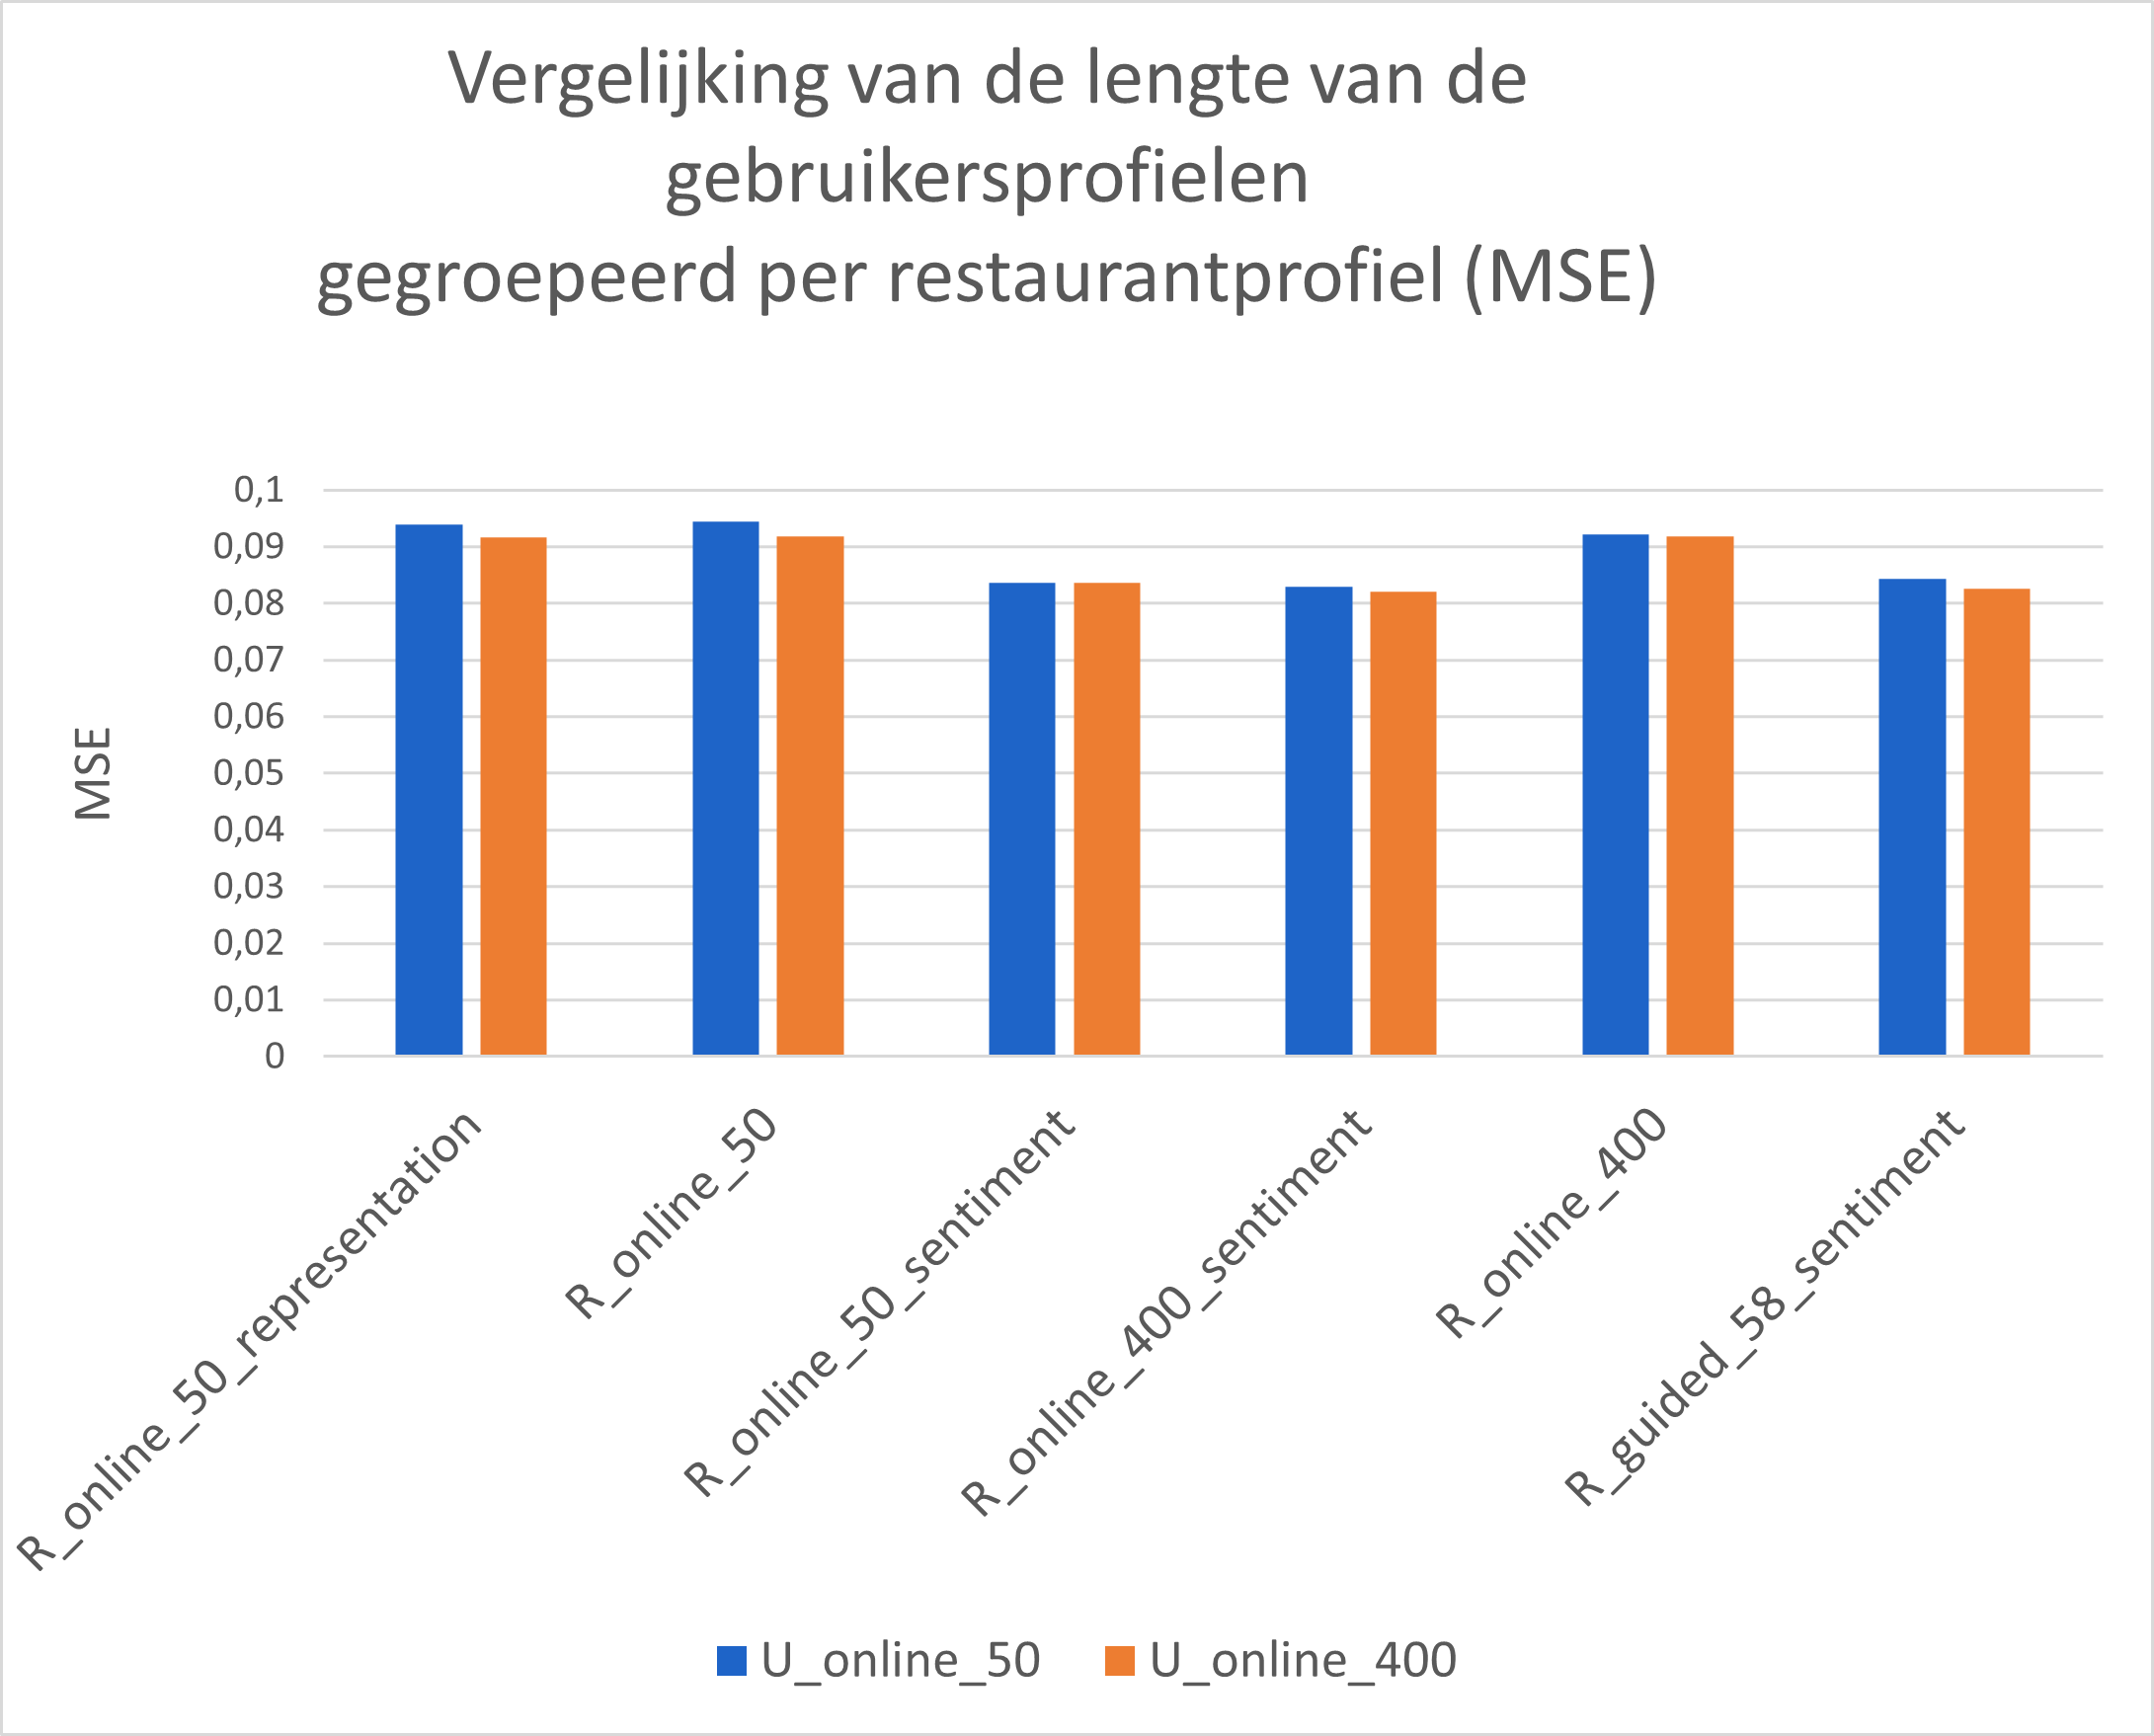
\includegraphics[width=\linewidth]{fig/chapt5/NLP/nlp_comparison_size_gebruiker.png}}\quad
        \parbox[b]{0.37\textwidth}{
        \subcaption{Gebruikersprofiel van 50 topics (blauw) en gebruikersprofiel van 400 topics (oranje) vergeleken met verschillende restaurantprofielen op basis van MSE.}\label{fig:chapt5_nlp_size_user}}
        \\[.5cm]

        \centering
        \parbox[b]{0.6\textwidth}{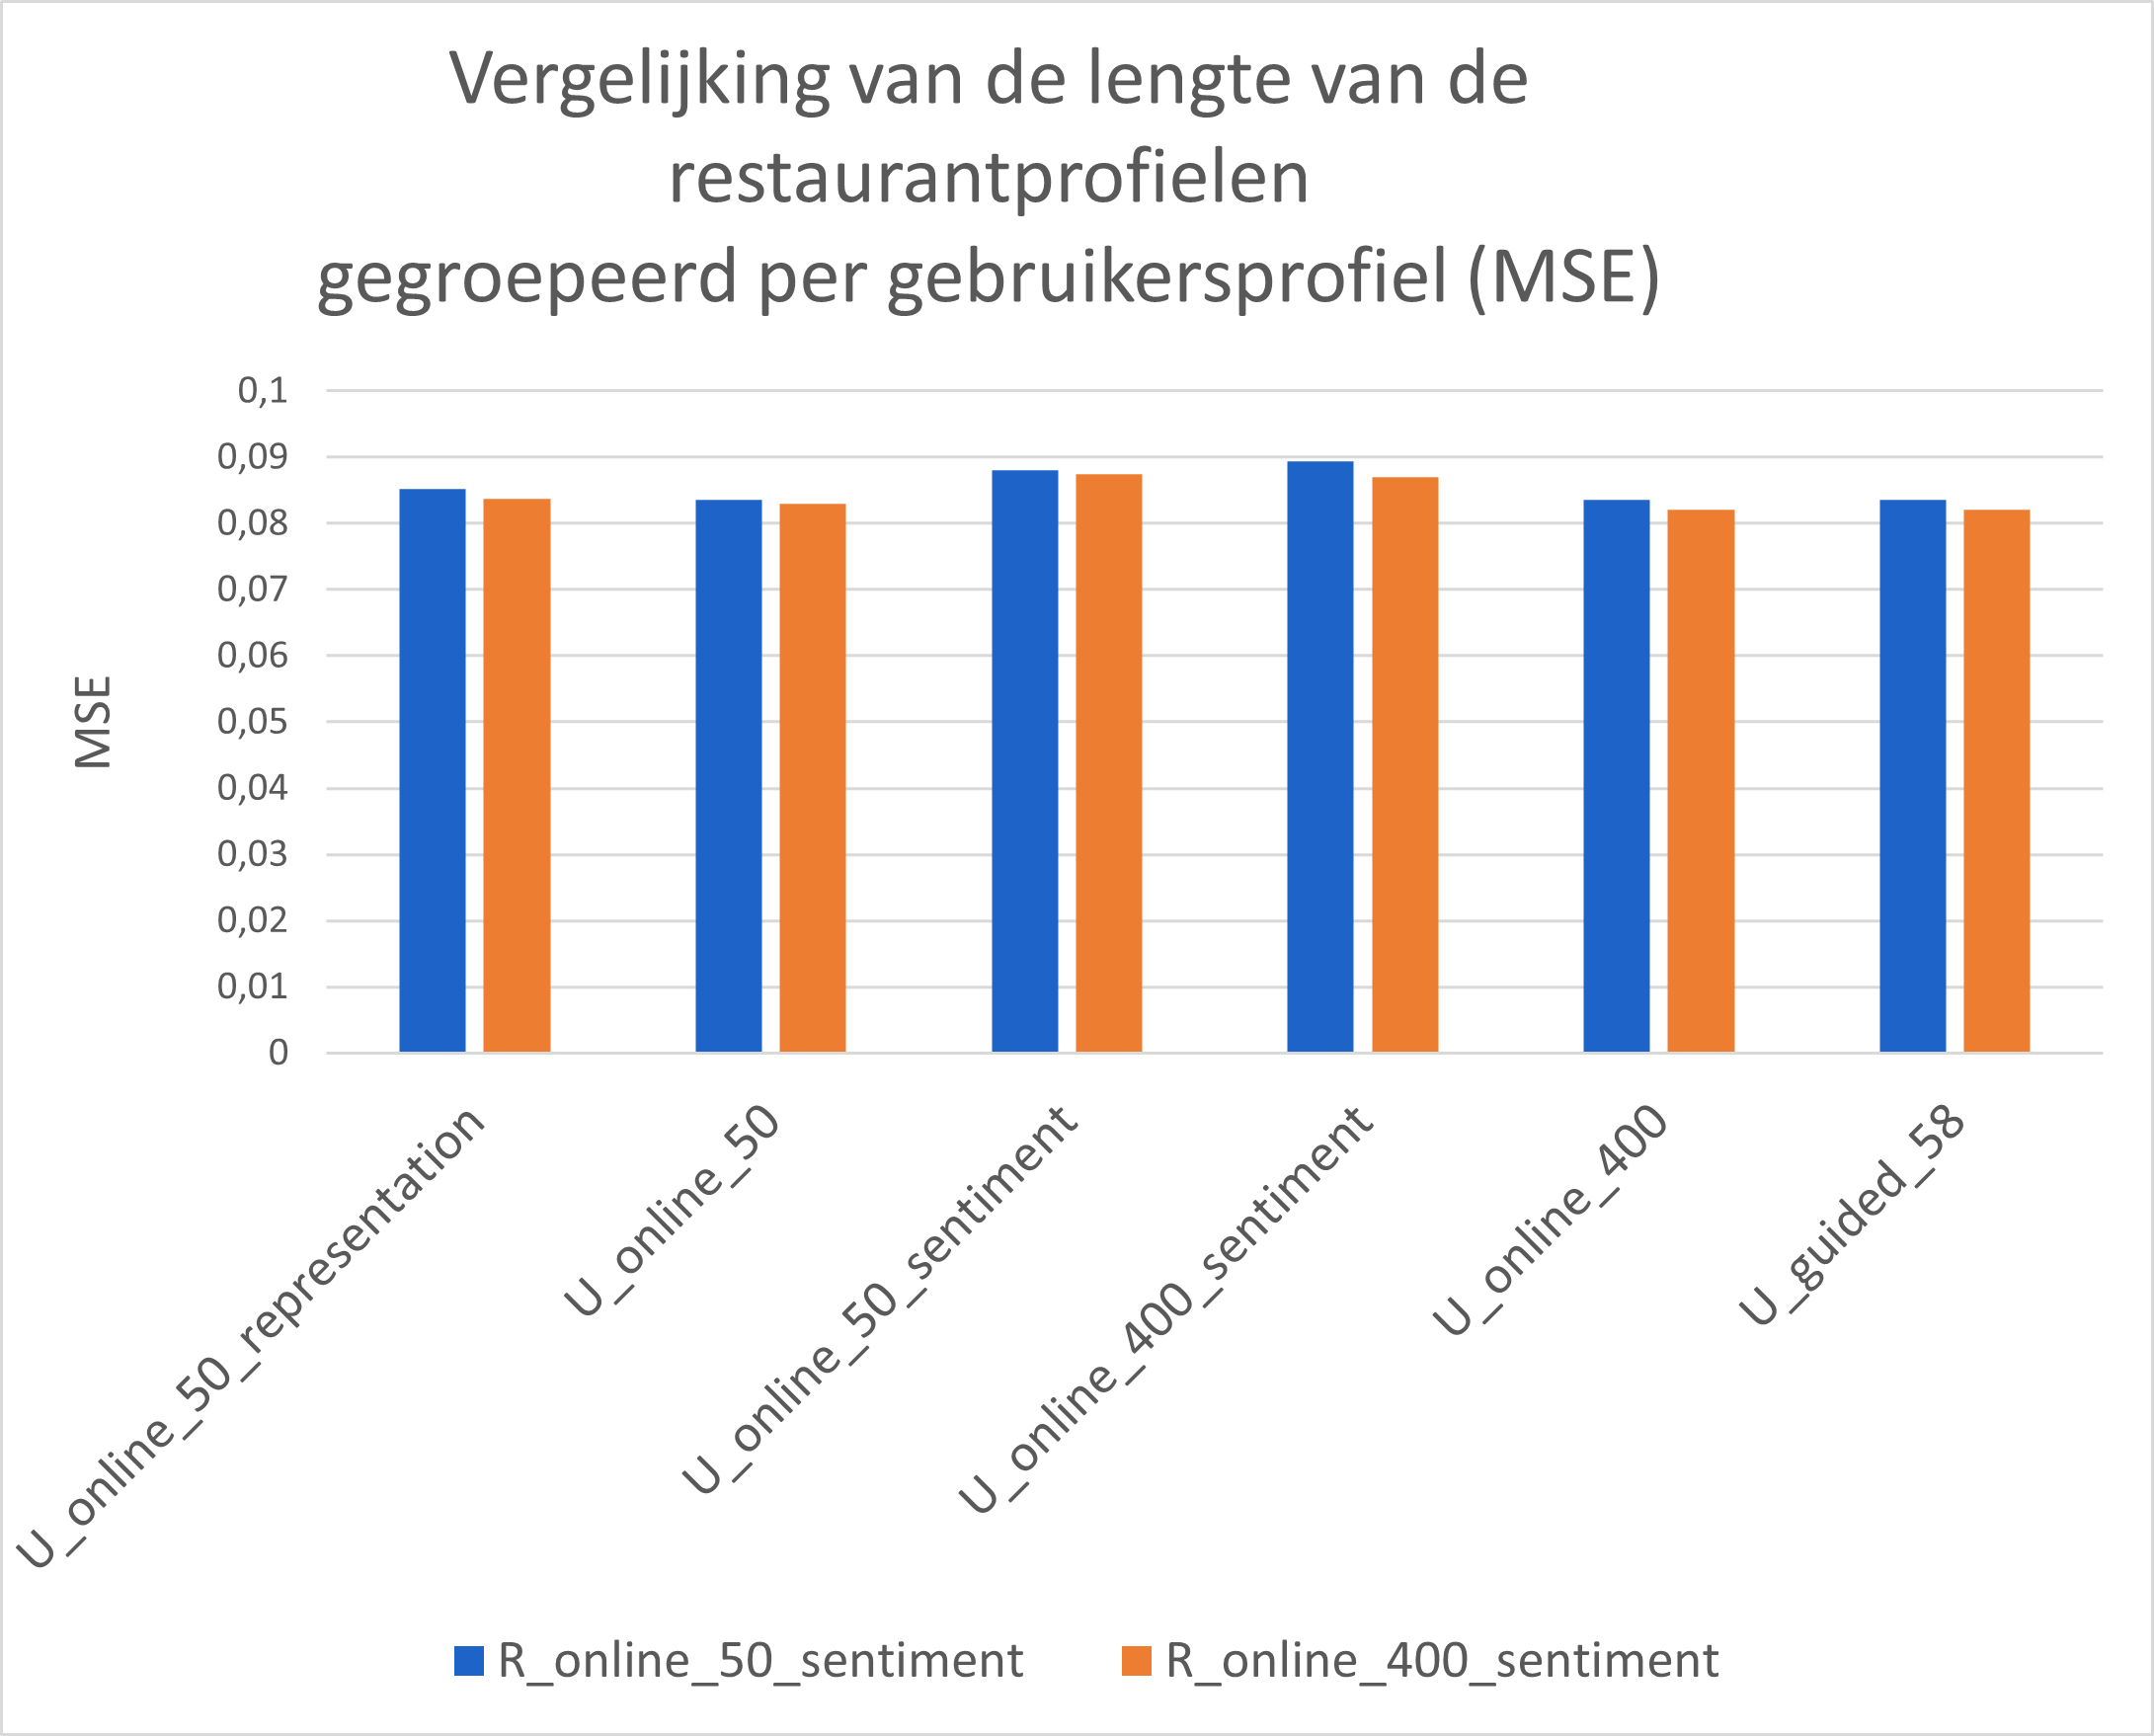
\includegraphics[width=\linewidth]{fig/chapt5/NLP/nlp_comparison_size_restaurant.png}}\quad
        \parbox[b]{0.37\textwidth}{
        \subcaption{Restaurantprofiel van 50 topics (blauw) en restaurantprofiel van 400 topics (oranje), beiden met sentiment, vergeleken met verschillende gebruikersprofielen op basis van MSE.}\label{fig:chapt5_nlp_size_restaurant}}
        \\[.5cm]

        \caption{Analyse van de impact van de lengte van gebruikers- en restaurantprofielen.}
        \label{fig:chapt5_nlp_size_model}
\end{figure}

De volgende hyperparameter die we bespreken is het aantal topics dat een model zal genereren. Dit is equivalent aan de lengte van één gebruikers- of restaurantprofiel. Door het gebruik van meer topics kan het model in het ideale geval specifieker zijn per topic. Hierdoor is het mogelijk om een duidelijker beeld te krijgen van een gebruiker of restaurant. In \autoref{fig:chapt5_nlp_size_model} gaan we twee gelijke modellen, met uitzondering van het aantal topics, met elkaar vergelijken. We concluderen dat het model van 400 topics niet significant beter is dan het model van 50 topics. Een mogelijke verklaring is dat het embeddingsmodel van BERTopic niet gefinetuned is: het gevolg hiervan is dat woorden zoals pasta en pizza toch in één topic samengevoegd worden. In het ideale geval worden deze afgesplitst zodat we hiervoor een onderscheid kunnen maken per gebruiker of restaurant.

Een laatste experiment is het manueel wegfilteren van bepaalde topics die niet relevant zijn voor een gebruikers- of restaurantprofiel. Dit is nuttig indien we de representatie van modellen gebruiken aangezien we hier een top $n$ selecteren. In het geval dat we de clustering van het model gebruiken, worden de waarden overeenkomend met de verwijderde topics op nul gezet. Dit komt overeen met bepaalde features weg te laten uit een neuraal netwerk. Met deze reden zullen we bij dit experiment focussen op de profielen op basis van representatie. \\

% filter topics \label{fig:chapt5_nlp_filter}
\mijnfiguur[H]{width=10cm}{fig/chapt5/NLP/nlp_comparison_filter.png}{Vergelijking van profielen van 400 topics waarbij er manueel topics weggefilterd kunnen worden}{fig:chapt5_nlp_filter}

Tijdens ons onderzoek hebben we manueel de relevante topics gefilterd van een online model met 400 topics. Vervolgens hebben we in \autoref{fig:chapt5_nlp_filter} de performantie van de profielen met aangepaste topics vergeleken met de originele. We maken een onderscheid tussen niet filteren, enkel gebruikersprofielen filteren, enkel restaurantprofielen filteren en ten slotte beide filteren. We merken op dat na het manueel filteren van topics de performantie daalt.

We kunnen concluderen dat er meerdere mogelijkheden zijn om goede gebruikers- en restaurantprofielen te genereren. Het BERTopic-model dat de beste resultaten geeft is online\_400, maar online\_50 en guided\_58 sluiten daar dicht bij aan. Ook voor de manier waarop we het model gebruiken, namelijk via de clustering of de representatie, is er weinig verschil. Het manueel wegfilteren van topics voegt subjectiviteit toe en heeft een negatieve impact op performantie. Deze techniek kunnen we dus uitsluiten voor het maken van de beste profielen. Ten slotte is de meest impactvolle toevoeging het gebruik van sentiment in de restaurantprofielen. Hiermee zien we een significante toename in performantie.\newline
Voor de experimenten in \autoref{sec:chapt5_neuraal_netwerk} maken we gebruik van de beste gebruikers- en restaurantprofielen. Beiden worden gegenereerd aan de hand van de clustering van een online\_400 model, waarbij sentiment wordt toegevoegd aan de restaurantprofielen.

\subsection{Verband tussen verschillende evaluatiemethoden}
\label{sub:chapt5_compare_eval_methods}
Nu we hebben vastgelegd welke modellen goede en slechte gebruikers- en restaurantprofielen genereren kunnen we deze vergelijken met de resultaten van de clusteringsmetrieken. Ondanks het feit dat Calinski-Harabasz score efficiënt te berekenen is, hangt deze af het aantal topics waardoor het vergelijken complex wordt. Hierdoor zullen we enkel gebruik maken van de Davies-Bouldin score en silhouette score. We vergelijken de resultaten uit \autoref{sub:chapt4_eval_clustering} met de MSE van gebruikers- en restaurantprofielen, gegenereerd aan de hand van de clustering van verschillende modellen, gecombineerd met sentiment analysis voor de restaurantprofielen.

\mijnfiguur[H]{width=14cm}{fig/chapt5/NLP/nlp_comparison_davies.png}{Verband tussen MSE en de Davies-Bouldin score voor verschillende BERTopic-modellen (lagere scores zijn beter)}{fig:chapt5_nlp_davies}

In \autoref{fig:chapt5_nlp_davies} merken we op dat de Davies-Bouldin score en MSE in het algemeen dezelfde trend volgen. De enige uitzondering is het model online\_400\_HD. Bij dit model is de dimensie hoger voordat er geclusterd wordt. Maar dit is niet het geval bij de MSE: deze ligt in lijn met de andere goede modellen. We nemen waar dat clusteren met een hogere dimensie een aanzienlijke impact heeft op de uitkomst van de Davies-Bouldin score. 

\mijnfiguur[H]{width=14cm}{fig/chapt5/NLP/nlp_comparison_silhouette.png}{Verband tussen MSE en de silhouette score voor verschillende BERTopic-modellen.}{fig:chapt5_nlp_silhouette}

De tweede metriek die we vergelijken is de silhouette score. Merk op een betere MSE score overeenkomt met een lagere waarde, maar bij de silhouette score is een hogere score beter. Indien we hiermee rekening houden kunnen we uit \autoref{fig:chapt5_nlp_silhouette} dezelfde conclusie trekken als bij de vergelijking met de Davies-Bouldin score.

We concluderen dat de resultaten van de clusteringsmetrieken een goede indicatie geven over de uiteindelijke performantie van een model. Hierbij moeten we opletten voor factoren die deze metrieken kunnen beïnvloeden, zoals de grootte van de dimensie voor het clusteren. Tot slot vermelden we dat aan de hand van deze metrieken enkel de performantie van de verschillende BERTopic modellen geëvalueerd kan worden. Externe manipulaties zoals sentiment analysis kunnen niet geëvalueerd worden door deze metrieken. Hiervoor moeten we gebruik maken de evaluatiemethoden van het neuraal netwerk zoals beschreven in \autoref{sub:chapt4_testsetup}.

























\section{Neuraal netwerk}
\label{sec:chapt5_neuraal_netwerk}
Op dit punt hebben we aan de hand van een basisimplementatie van het neuraal netwerk de beste combinatie gevonden voor de inputprofielen. We keren eerst even terug naar de aanpassingen die we maakten aan het basismodel, zoals uitgelegd in de inleiding van dit hoofdstuk: na het opstellen van alle mogelijke implementaties van gebruikers- en restaurantprofielen merkten we op dat het neuraal netwerk niet in staat was om verbanden te capteren. Doordat het model na meer dan 400 epochs nog heel vaak terugviel op een voorspelling van 4 op 5, leek het aangewezen om de optimizer en diens parameters aan te passen.

We probeerden verschillende learning rates met SGD, en hoewel dit een effect had op het trainingsproces, slaagden we er niet in om een geschikte waarde te vinden. Een kleine learning rate zorgde dat het model niets leerde. Bij grotere learning rates was het model zeer instabiel waardoor het geen verbeterde voorspellingscapaciteit opleverde na trainen over meerdere epochs (\autoref{fig:chapt5_sgd_slecht_loss}).

Doordat de ADAGRAD-optimizer dynamisch de learning rate kan aanpassen, is deze methode stabieler. We zien dit gedrag terug in \autoref{fig:chapt5_adagrad_goed}, waarbij we vinden dat een initiële learning rate van $0.0002$ de beste resultaten geeft. Hoewel de loss natuurlijk voor iedere combinatie van NLP-profielen anders is, blijft de conclusie wel hetzelde: SGD is te willekeurig en onstabiel, ADAGRAD is stabieler en scoort een (iets) lagere loss. Hierdoor kozen we om deze optimizer te gebruiken bij het evalueren van de NLP-profielen.

\begin{figure}[H]
    \begin{subfigure}{.45\textwidth}
        \centering
        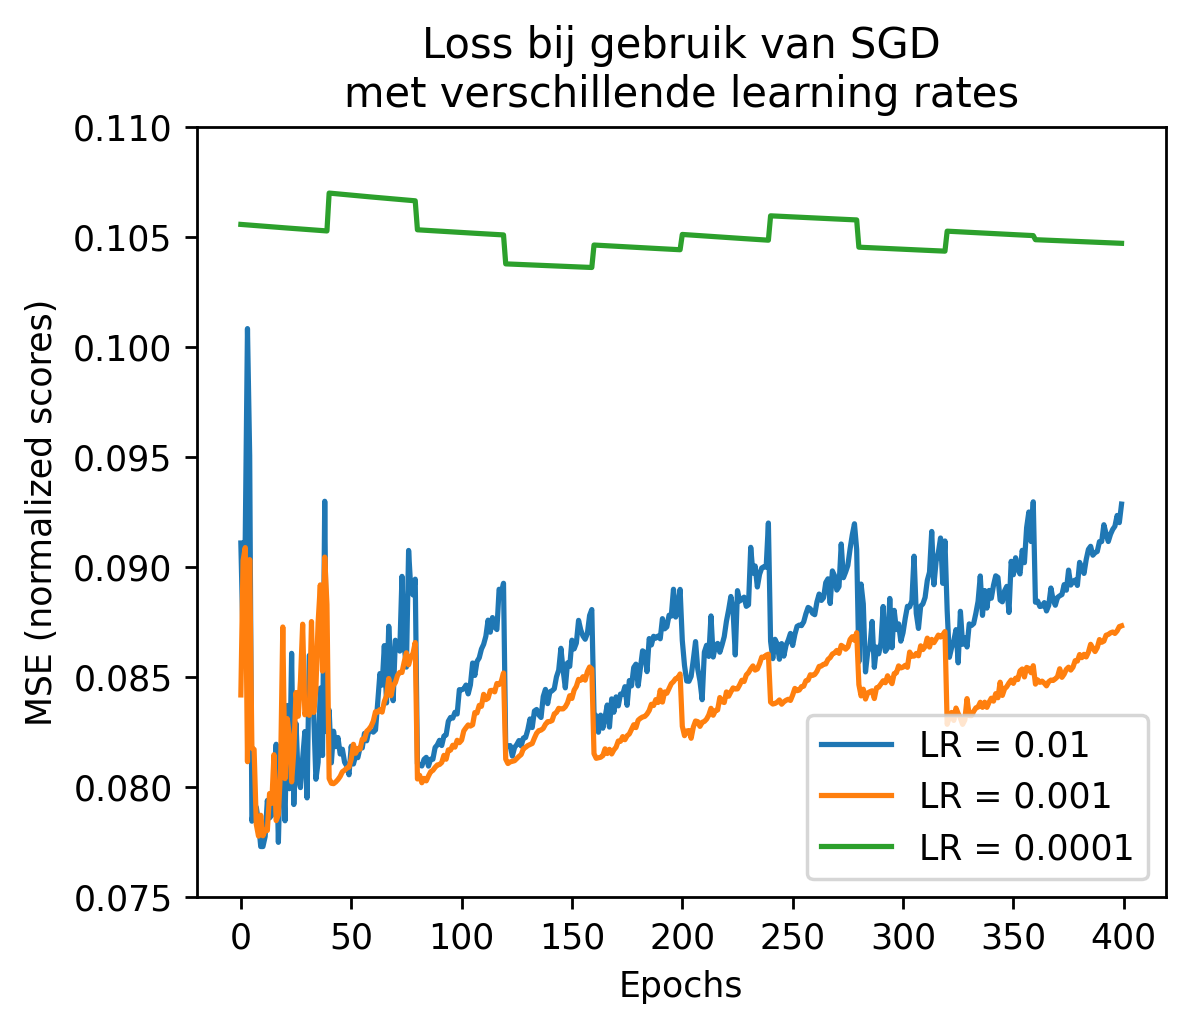
\includegraphics[width=1\linewidth]{fig/chapt5/predictor/sgd_slecht.png}
        \caption{SGD}
        \label{fig:chapt5_sgd_slecht_loss}
    \end{subfigure}
    \begin{subfigure}{.45\textwidth}
        \centering
        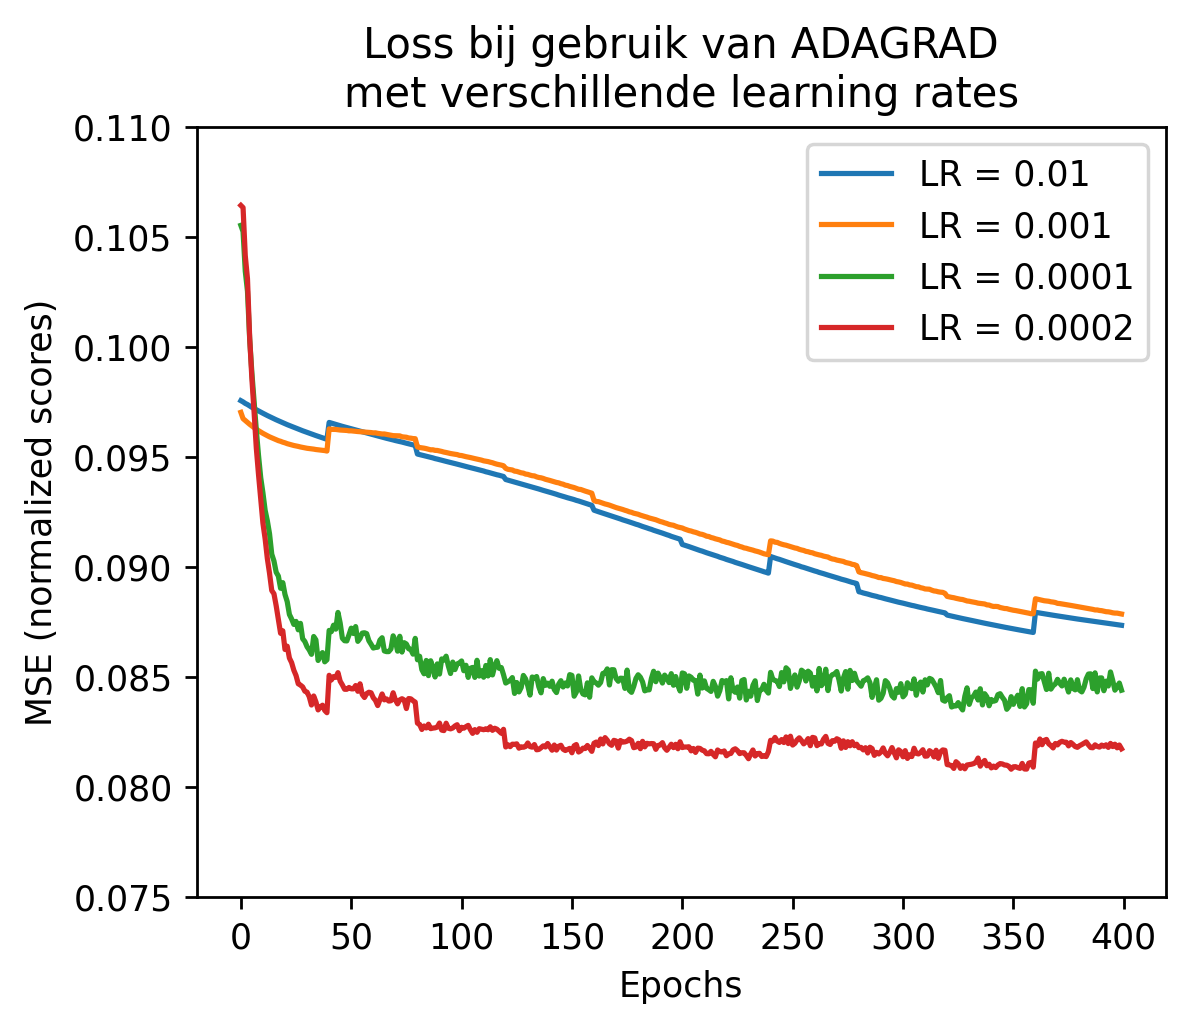
\includegraphics[width=1\linewidth]{fig/chapt5/predictor/adagrad_goed.png}
        \caption{ADAGRAD}
        \label{fig:chapt5_adagrad_goed}
    \end{subfigure}
    \caption{SGD slaagt er niet in om het model verbanden aan te leren, ADAGRAD wel}
    \label{fig:chapt5_sgd_adagrad_combined}
\end{figure}

Merk op dat naar mate het aantal afgewerkte epochs toeneemt, het hergebruiken van dezelfde datasplit minder effectief wordt bij (ADAGRAD, $0.0002$). Bij al deze modellen is dezelfde datasplit steeds 40 epochs op rij gebruikt. We nemen hieruit mee dat er frequenter van datasplit mag veranderd worden. We gebruiken bij alle volgende experimenten 20 epochs per datasplit.\newline
Alle volgende experimenten zullen we alleen toepassen op de netwerken getraind met de best beschikbare inputvector, die onder andere bestaat uit de gebruikers- en restaurantprofielen zoals beschreven in \autoref{sub:chapt5_nlp_resultaten}.

In de volgende secties onderzoeken we verschillende eigenschappen en parameters van het neuraal netwerk. We maken hierbij de assumptie dat parameters onafhankelijk zijn van elkaar, en dat we deze individueel kunnen optimaliseren. In realiteit zal dit niet altijd kloppen. Echter zou een volledige grid search over alle parameters en inputprofielen computationeel veel te zwaar zijn.

\subsection{Architectuur neuraal netwerk}
De complexiteit van het netwerk heeft een directe impact op de performantie. De uitgebreidere netwerken scoren betere resultaten. Het beste resultaat wordt gescoord door het model met zes verborgen lagen. Merk op dat er vanaf het model met vijf verborgen lagen een merkbare sprong zit in de resultaten. Dit komt waarschijnlijk doordat de eerste verborgen laag van deze modellen meer neuronen bevat dan de inputlaag. Dit lijkt een zeer positieve invloed te hebben op de resultaten.

\mijnfiguur[H]{width=16cm}{fig/chapt5/predictor/loss_verschillende_architecturen.png}{Vergelijking van verschillende architecturen}{fig:chapt5_loss_verschillende_architecturen}

We definiëren een voorspelling als \q{correct} als de voorspelde waarde na afronding gelijk is aan de echte waarde. Deze afronding weerspiegelt de mogelijke waarden waaruit de gebruiker kan kiezen. De accuraatheid van een model is dan het percentage van correcte voorspellingen. Een analyse van de voorspellingen toont aan dat er een verband is tussen de loss en de accuraatheid van een model. Hoewel dit intuïtief klinkt, kan het zijn dat een model consistent 1 ster naast de echte waarde voorspelt, en toch een lage loss behaalt. Dit is bij ons niet het geval. \autoref{fig:chapt5_accuracy_all_architectures} toont aan dat de complexere modellen een hogere accuraatheid scoren, in lijn met het verschil in loss (\autoref{fig:chapt5_loss_verschillende_architecturen}). \autoref{fig:chapt5_accuracy_6_layers} toont de gemaakte fouten bij het beste model. We zien dat het model hoofdzakelijk een fout van 1 ster maakt.

\begin{figure}[H]
    \begin{subfigure}{.45\textwidth}
        \centering
        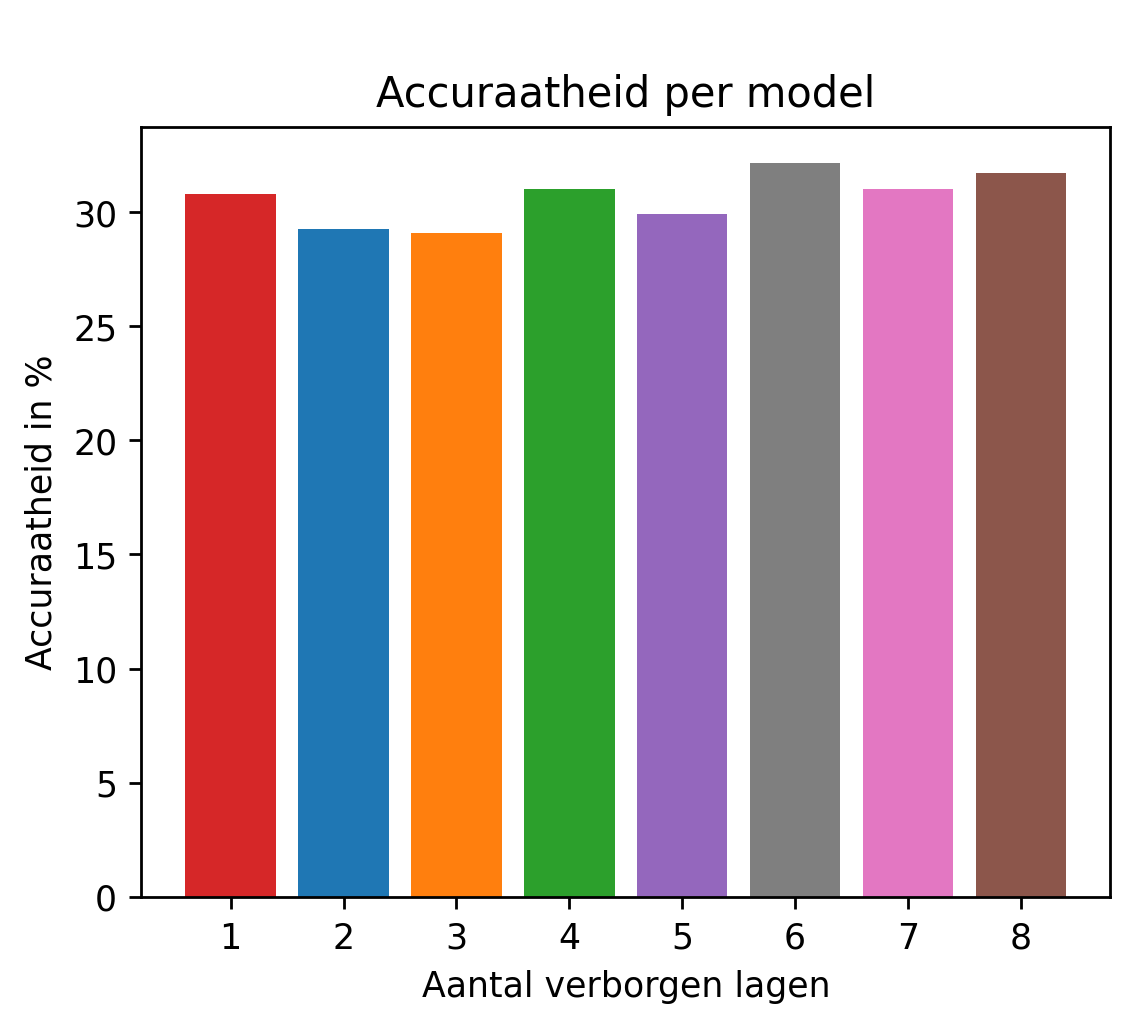
\includegraphics[width=1\linewidth]{fig/chapt5/predictor/accuracy_per_model.png}
        \caption{De accuraatheid van iedere architectuur}
        \label{fig:chapt5_accuracy_all_architectures}
    \end{subfigure}
    \begin{subfigure}{.45\textwidth}
        \centering
        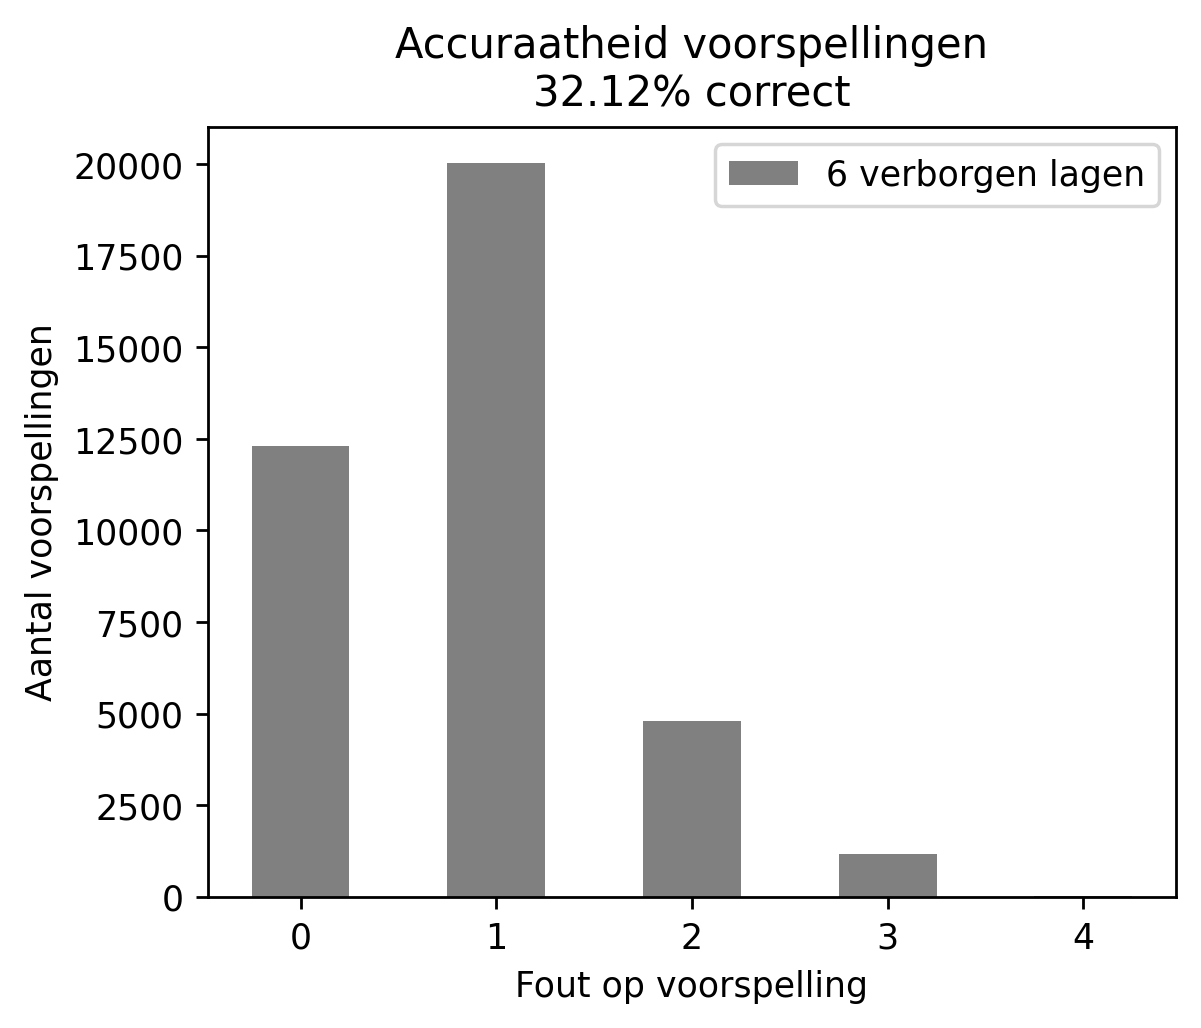
\includegraphics[width=1\linewidth]{fig/chapt5/predictor/accuracy_32.12_6_layers_hist.png}
        \caption{Histogram fouten bij model met 6 verborgen lagen}
        \label{fig:chapt5_accuracy_6_layers}
    \end{subfigure}
    \caption{Accuraatheid van modellen}
    \label{fig:chapt5_accuracy_architectures}
\end{figure}


Ieder model, inclusief het meest eenvoudige, lijkt wel effectief te leren op basis van de inputfeatures, en voorspelt dus niet steeds naïef 4 van de 5 sterren. Zo zien we de voorspellingen van het model met één verborgen laag terug in \autoref{tab:chapt5_simpel_model_voorspellingen}. Merk op dat we de voorspellingen afronden. 

\begin{table}[H]
    \centering
    \begin{tabular}{l|l|l|l}
       & Voorspelling & Echte waarde & Verschil   \\ \hline
    0  & 4            & 3            & \textbf{1} \\
    1  & 4            & 3            & \textbf{1} \\
    2  & 4            & 4            & \textbf{0} \\
    3  & 4            & 4            & \textbf{0} \\
    4  & 5            & 4            & \textbf{1} \\
    5  & 3            & 2            & \textbf{1} \\
    6  & 3            & 2            & \textbf{1} \\
    7  & 4            & 4            & \textbf{0} \\
    8  & 4            & 5            & \textbf{1} \\
    9  & 4            & 4            & \textbf{0} \\
    10 & 5            & 5            & \textbf{0}
    \end{tabular}
    \caption{Voorspellingen voor het model met 1 verborgen laag}
    \label{tab:chapt5_simpel_model_voorspellingen}
\end{table}




We stellen ook opnieuw het effect vast van het hergebruiken van dezelfde inputvectoren voor 20 epochs: er is een klein maar meetbaar verschil in MSE. De veronderstelling dat we meerdere epochs kunnen trainen met dezelfde datasplit blijft wel gelden: we zien bijvoorbeeld dat de loss daalt tussen epoch 80 en 100 hoewel we trainen op dezelfde data, en we zien dat er toch een generaliteit wordt aangeleerd omdat bij een volgende datasplit het verschil in loss beperkt blijft.\newline
Bij de complexere modellen is er al sprake van convergentie bij de loss na ongeveer 100 epochs. Bij de modellen met maximaal vier verborgen lagen is dit pas na meer dan 250 epochs het geval. Dit ligt niet in lijn met een veronderstelde eigenschap van deze neurale netwerken, die stelt dat complexere netwerken trager convergeren tijdens het trainen. We vinden geen verklaring voor dit fenomeen.

We concluderen dat de beste resultaten worden behaalt met een model dat bestaat uit 6 verborgen lagen. De volledige architectuur ziet er dan uit als in \autoref{fig:chapt5_best_network}.

\mijnfiguur[H]{width=16cm}{fig/chapt5/predictor/best_network.png}{Voorstelling van de architectuur met zes verborgen lagen, waarbij $n$ het aantal inputfeatures voorstelt}{fig:chapt5_best_network}





\subsection{Invloed NLP-profielen}
\label{sec:chapt5_invloed_nlp_profielen}
We bestuderen de impact van de NLP-profielen op de loss van het neuraal netwerk. Eerst meten we hoe goed het netwerk presteert zonder deze extra inputfeatures. Met andere woorden, we baseren de voorspellingen enkel op de gelabelde dataset. We proberen ook combinaties, waarbij enkel de NLP-gebruikersprofielen of NLP-restaurantprofielen worden toegevoegd aan de gelabelde data. De resultaten staan in \autoref{fig:chapt5_invloed_NLP}. We merken op dat de NLP-gebruikersprofielen een veel grotere impact hebben dan de NLP-restaurantprofielen. Het lijkt er dus op dat de gelabelde data de restaurants reeds voldoende beschrijven om verbanden te maken. Aangezien we op zoek zijn naar de best mogelijke performantie, gaan we verder met de combinatie van gebruikers- en restaurantprofielen gemaakt met zowel gelabelde als tekstuele data.

\mijnfiguur[H]{width=14cm}{fig/chapt5/predictor/invloed_NLP.png}{Loss voor verschillende combinaties van NLP-profielen}{fig:chapt5_invloed_NLP}


\subsection{Dimensionaliteitsreductie}
De huidige implementatie van het neuraal netwerk heeft een inputlaag bestaande uit $1000$ neuronen, waarvan 200 verbonden worden met gelabelde data, en 800 met NLP-profielen. Bij dit experiment passen we PCA toe op de volledige inputvector, om zo een dimensionaliteitsreductie van 1000 naar 400 uit te voeren. We onderzoeken ook PCA op enkel het NLP-restaurantprofiel, aangezien we in \autoref{sec:chapt5_invloed_nlp_profielen} ontdekten dat dit profiel relatief weinig invloed had op de voorspellingen, maar wel dimensie 400 heeft. PCA verkleint in dit geval de dimensie tot 150. Deze waarden stellen meer dan een halvering van dimensie voor, maar zijn overigens arbitrair gekozen. Uit \autoref{fig:chapt5_invloed_pca} besluiten we dat deze toepassing van PCA geen significante verbetering met zich meebrengt.

\mijnfiguur[H]{width=14cm}{fig/chapt5/predictor/invloed_pca.png}{Loss na toepassing van PCA op (een deel van) de inputvectors}{fig:chapt5_invloed_pca}


\subsection{Cold-Startprobleem}
We meten een stijging in accuraatheid bij gebruikers met meer reviews. Over de volledige dataset halen we een accuraatheid van 32,2\%. Bij gebruikers met maximaal vijf reviews ligt de accuraatheid op 22,01\%. Er is dus een significant verschil. We merken op dat er percentueel minder grote voorspellingsfouten voorkomen bij gebruikers met veel reviews. Een grotere hoeveelheid data per gebruiker biedt dus meer zekerheid. In een productieomgeving zouden we voor gebruikers met minder dan vijf reviews een aanpassing aan het model voorstellen: hierbij zouden populaire restaurants met een hoge gemiddelde score een groter gewicht hebben bij het genereren van aanbevelingen, daar ons model nog niet veel zekerheid kan bieden voor deze gebruikers.

Het is ook mogelijk dat gebruikers met veel reviews meer belang hechten aan hun Yelpaccount, en daarom meer kwalitatieve reviews achterlaten waar de NLP-algoritmen meer data uit kunnen extraheren.


\mijnfiguur[H]{width=10cm}{fig/chapt5/predictor/effect_coldstart_partities.png}{Evolutie in accuraatheid bij stijgend aantal reviews per gebruiker}{fig:chapt5_coldstart_partities}

\begin{figure}[H]
    \begin{subfigure}{.45\textwidth}
        \centering
        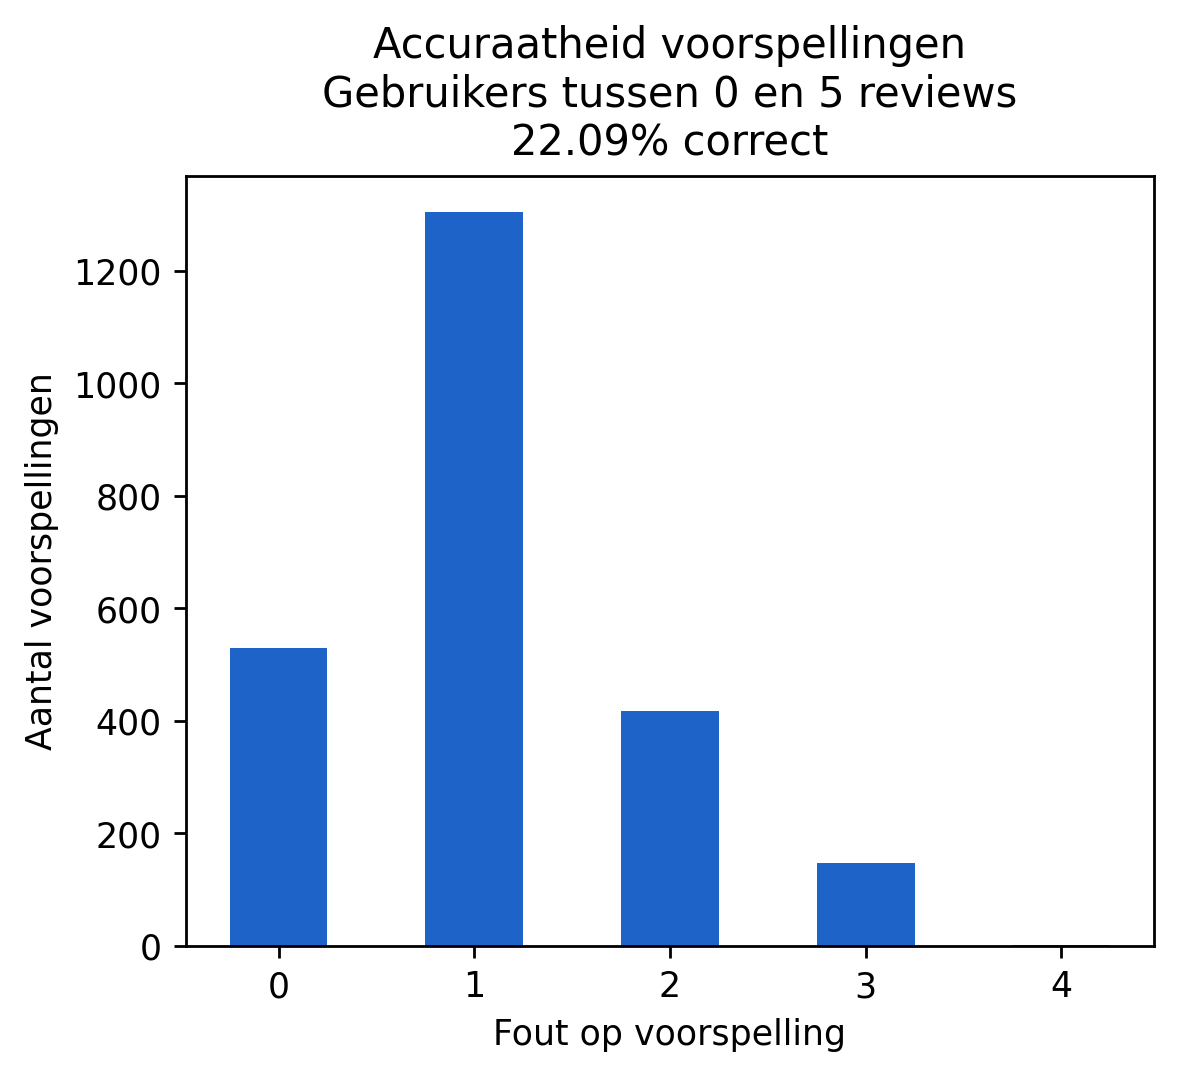
\includegraphics[width=1\linewidth]{fig/chapt5/predictor/accuracy_0_5.png}
    \end{subfigure}
    \begin{subfigure}{.45\textwidth}
        \centering
        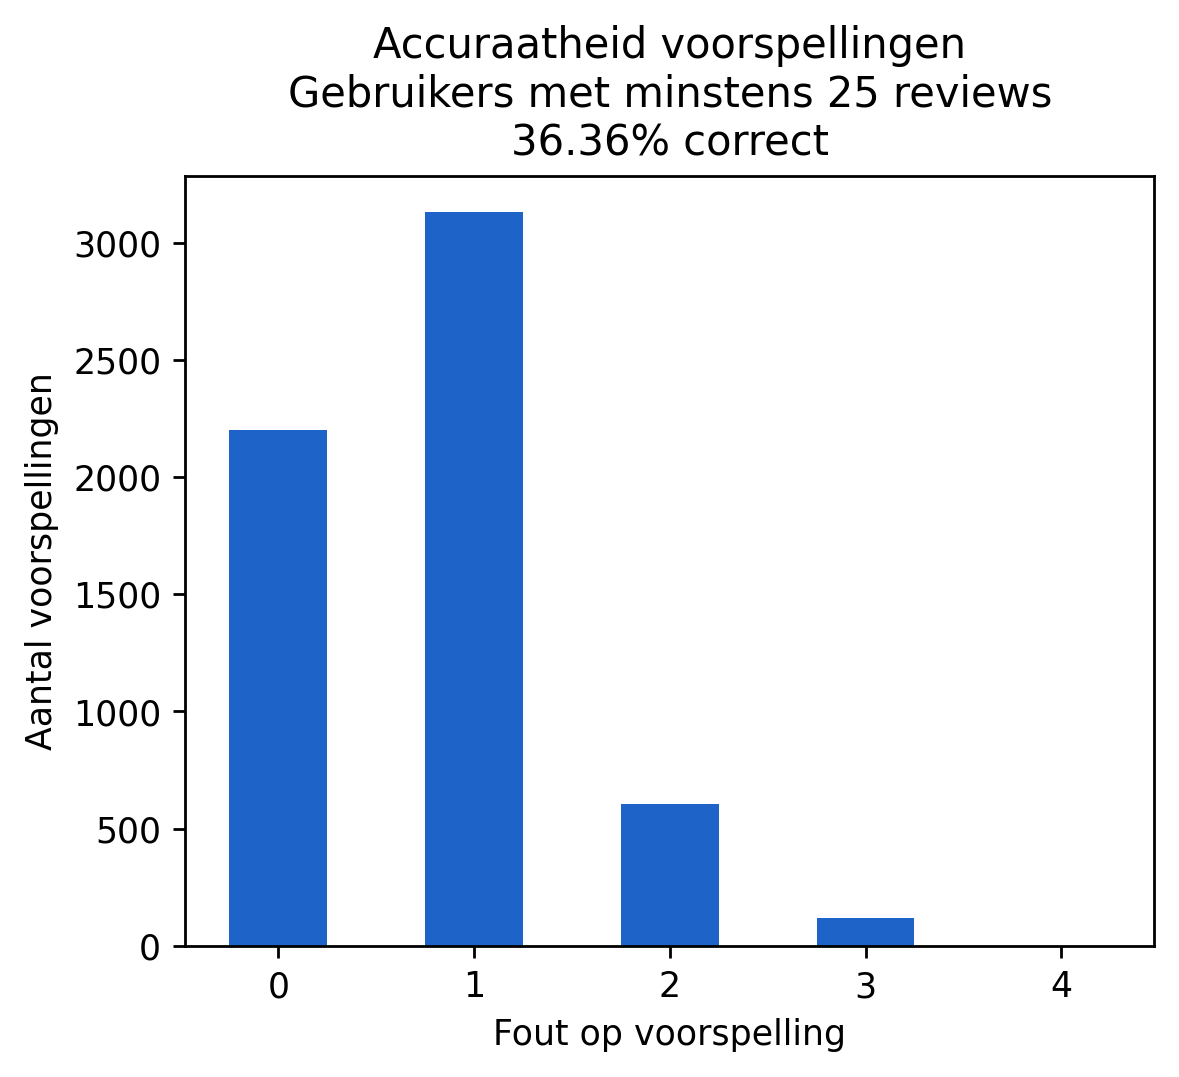
\includegraphics[width=1\linewidth]{fig/chapt5/predictor/accuracy_25+.png}
    \end{subfigure}
    \caption{Accuraatheid voor gebruikers met maximaal vijf reviews versus gebruikers met minimaal 25 reviews}
    \label{fig:chapt5_accuracy_coldstart}
\end{figure}

\subsection{Grootte dataset}
Na experimenten zien we dat het algoritme nog steeds goed presteert indien we slechts de helft van de originele trainset gebruiken om te trainen. Er zijn wel meer epochs nodig om de loss te laten convergeren. Dit is logisch, daar in één epoch er nu maar half zoveel informatie aanwezig is. Bij 25\% merken we dat het gebrek aan data een probleem vormt: overfitting vindt plaats, daar het model niet meer in staat is om algemene conclusies te capteren uit de beperkte trainset.

\mijnfiguur[H]{width=10cm}{fig/chapt5/predictor/loss_all_beperkte_data.png}{Loss voor verschillende groottes van trainset}{fig:chapt5_loss_all_beperkte_data}

\subsection{Extreme voorspellingen}
Het model neigt te vaak 4 op 5 sterren te voorspellen, aangezien deze waarde een \q{gouden middenweg} is: het ligt dichtbij de meest-voorkomende waarde van 5 op 5 sterren, maar ook dichter in de buurt bij de lagere scores. We verklaren het gebrek aan accuraatheid voor 1-ster reviews door de onbalans voor deze klasse in de dataset. Het is ook mogelijk dat deze reviews afwijkingen voorstellen die moeilijk te voorspellen zijn, zoals bijvoorbeeld \q{Extreem lange wachttijd} op een uitzonderlijk drukke dag, of \q{Gesloten}.

\begin{figure}[H]
    \begin{subfigure}{.30\textwidth}
        \centering
        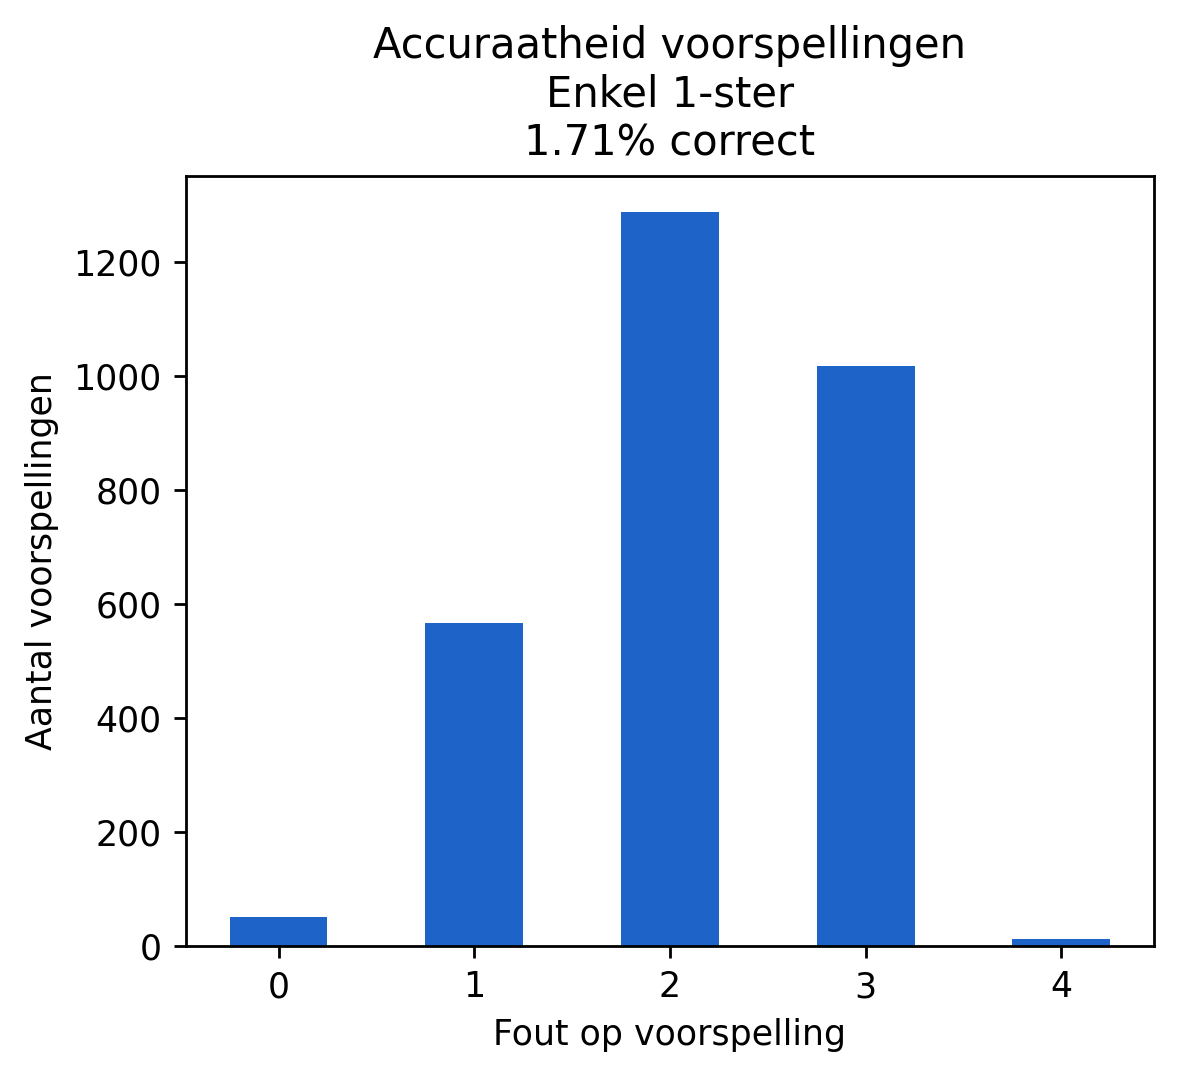
\includegraphics[width=1\linewidth]{fig/chapt5/predictor/extreem_1ster.png}
        \caption{Fouten bij 1 ster}
        \label{fig:chapt5_extreem_1ster}
    \end{subfigure}
    \begin{subfigure}{.30\textwidth}
        \centering
        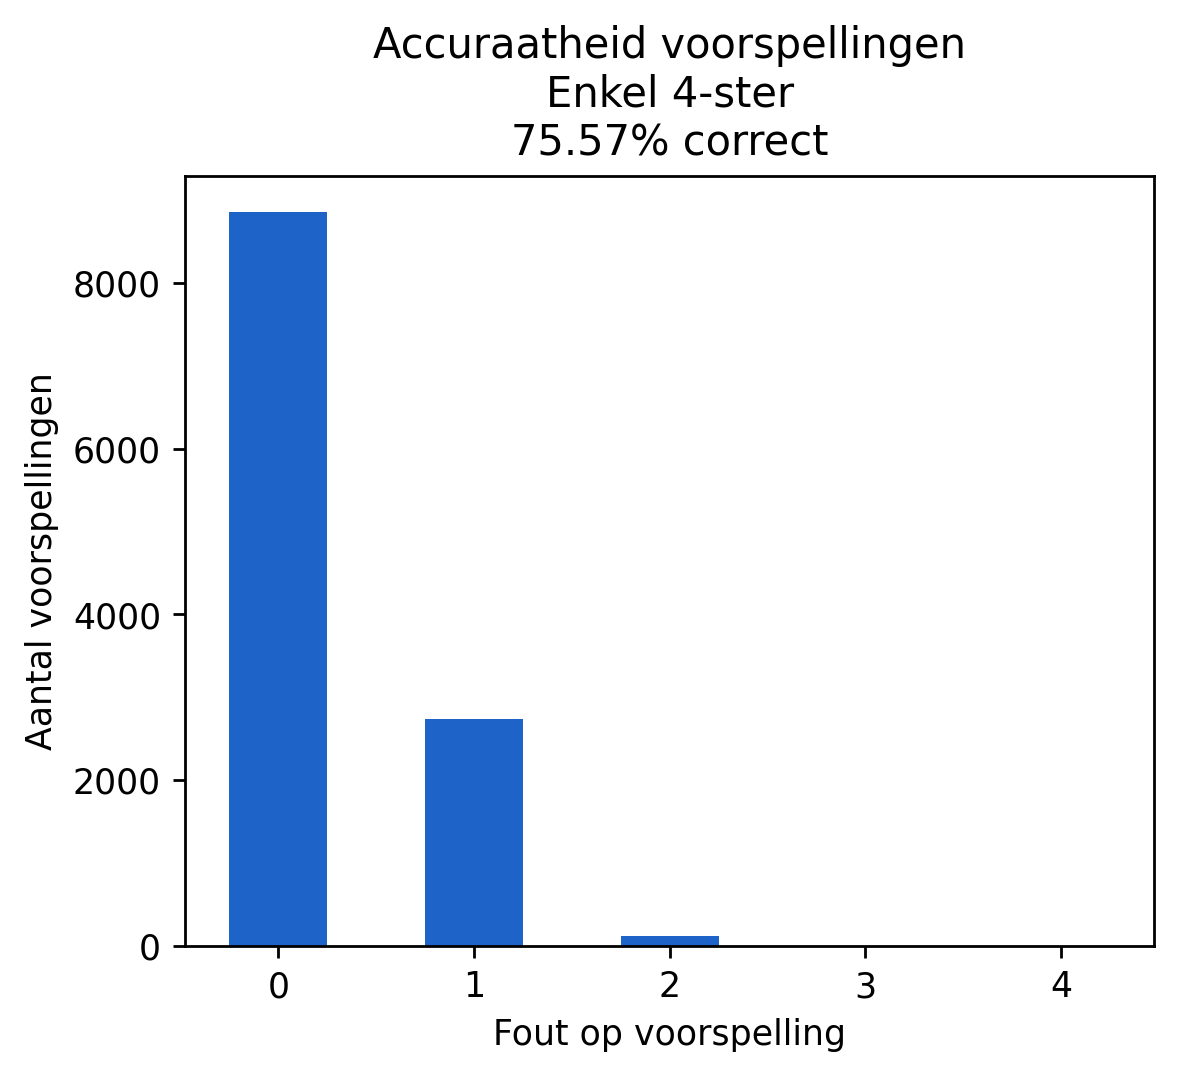
\includegraphics[width=1\linewidth]{fig/chapt5/predictor/extreem_4ster.png}
        \caption{Fouten bij 4 sterren}
        \label{fig:chapt5_extreem_4ster}
    \end{subfigure}
    \begin{subfigure}{.30\textwidth}
        \centering
        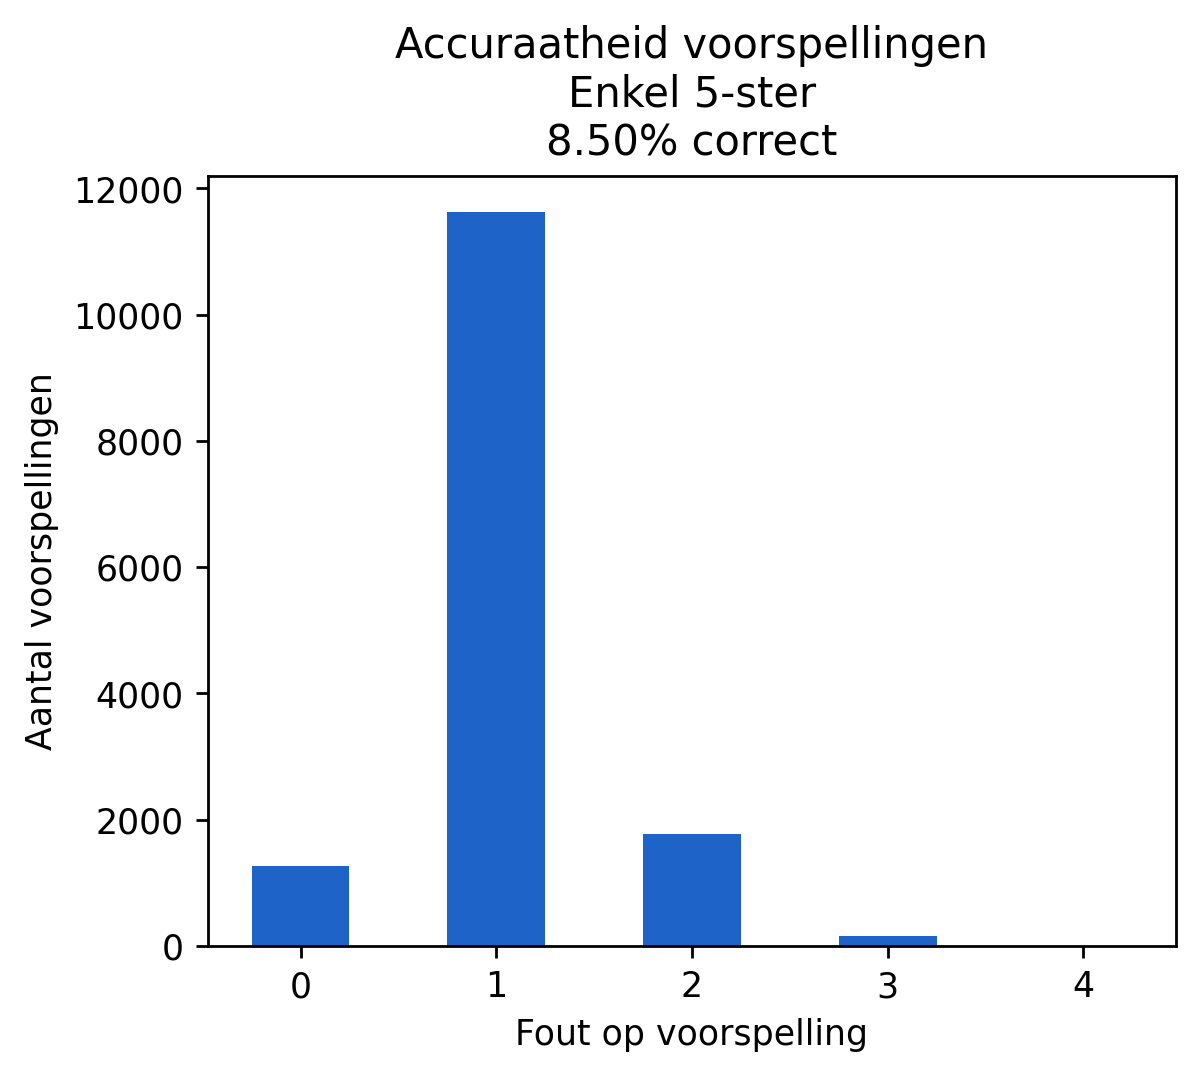
\includegraphics[width=1\linewidth]{fig/chapt5/predictor/extreem_5ster.png}
        \caption{Fouten bij 5 sterren}
        \label{fig:chapt5_extreem_5ster}
    \end{subfigure}
    \caption{Gemaakte fouten voor alle reviews uit de testset met een specifieke score}
    \label{fig:chapt5_extreme_scores}
\end{figure}



\subsection{Lossfuncties}
Het probleem waarbij het model te vaak conservatief een score van 4 sterren voorspelt kunnen we proberen oplossen met een aangepaste lossfunctie. Om makkelijk de resultaten te kunnen vergelijken, wordt deze lossfunctie enkel gebruikt tijdens het trainen van het netwerk, en niet tijdens het testen.

Een eerste alternatief zal de lossfunctie sneller laten stijgen, zodat kleine fouten een grotere straf krijgen. Het idee is dat het model zo meer geforceerd wordt om niet steeds 4 te voorspellen omdat de loss te groot wordt.\newline
Een tweede idee zal het extra gewichten toekennen aan ondergerepresenteerde klassen. Reviews die 1, 2, of 3 sterren hebben zullen 60\% meer doorwegen. Reviews met 5 sterren zullen 10\% meer doorwegen. Hierdoor proberen we opnieuw het model aan te leren om meer diverse scores te voorspellen.\newline

De resultaten tonen dat het eerste alternatief de loss marginaal naar beneden krijgt. Het toekennen van extra gewichten om de onbalans te remediëren lijkt niet te werken. Het model is hierbij niet in staat om verbanden te ontdekken tussen de output van de lossfunctie en de gewichten van de neuronen. We probeerden verschillende waarden voor de gewichten, maar sloegen er niet in om betere resultaten te behalen.

Geen van beide alternatieve lossfuncties loste het probleem op waarbij het model een extreem lage accuraatheid haalt op ondergerepresenteerde klassen. In tegendeel, de accuraatheid voor reviews met 1 ster gaat naar beneden (\autoref{fig:chapt5_accuracy_lossfunction_combined}). We besluiten daarom om deze varianten op de MSE niet te gebruiken.



\mijnfiguur[H]{width=14cm}{fig/chapt5/predictor/lossfuncties_samen.png}{Vergelijking van verschillende lossfuncties}{fig:chapt5_lossfuncties_samen}

\begin{figure}[H]
    \begin{subfigure}{.45\textwidth}
        \centering
        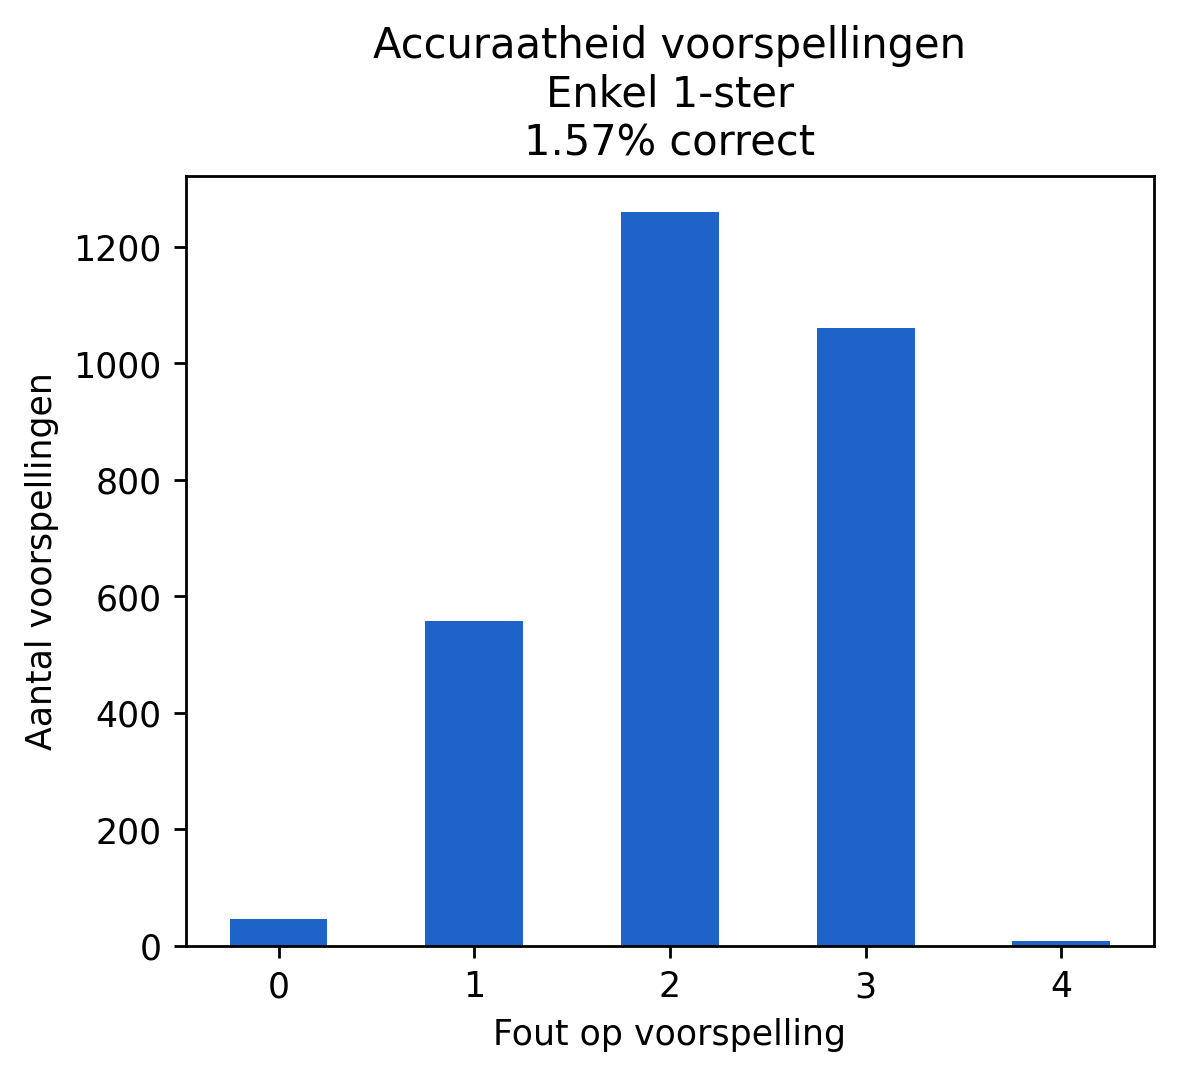
\includegraphics[width=1\linewidth]{fig/chapt5/predictor/1ster_nieuwe_loss.png}
        \caption{Alternatief 1: {\fontfamily{qcr}\selectfont mean(5 * error²)}}
        \label{fig:chapt5_extreem_1ster_nieuwe_loss}
    \end{subfigure}
    \begin{subfigure}{.45\textwidth}
        \centering
        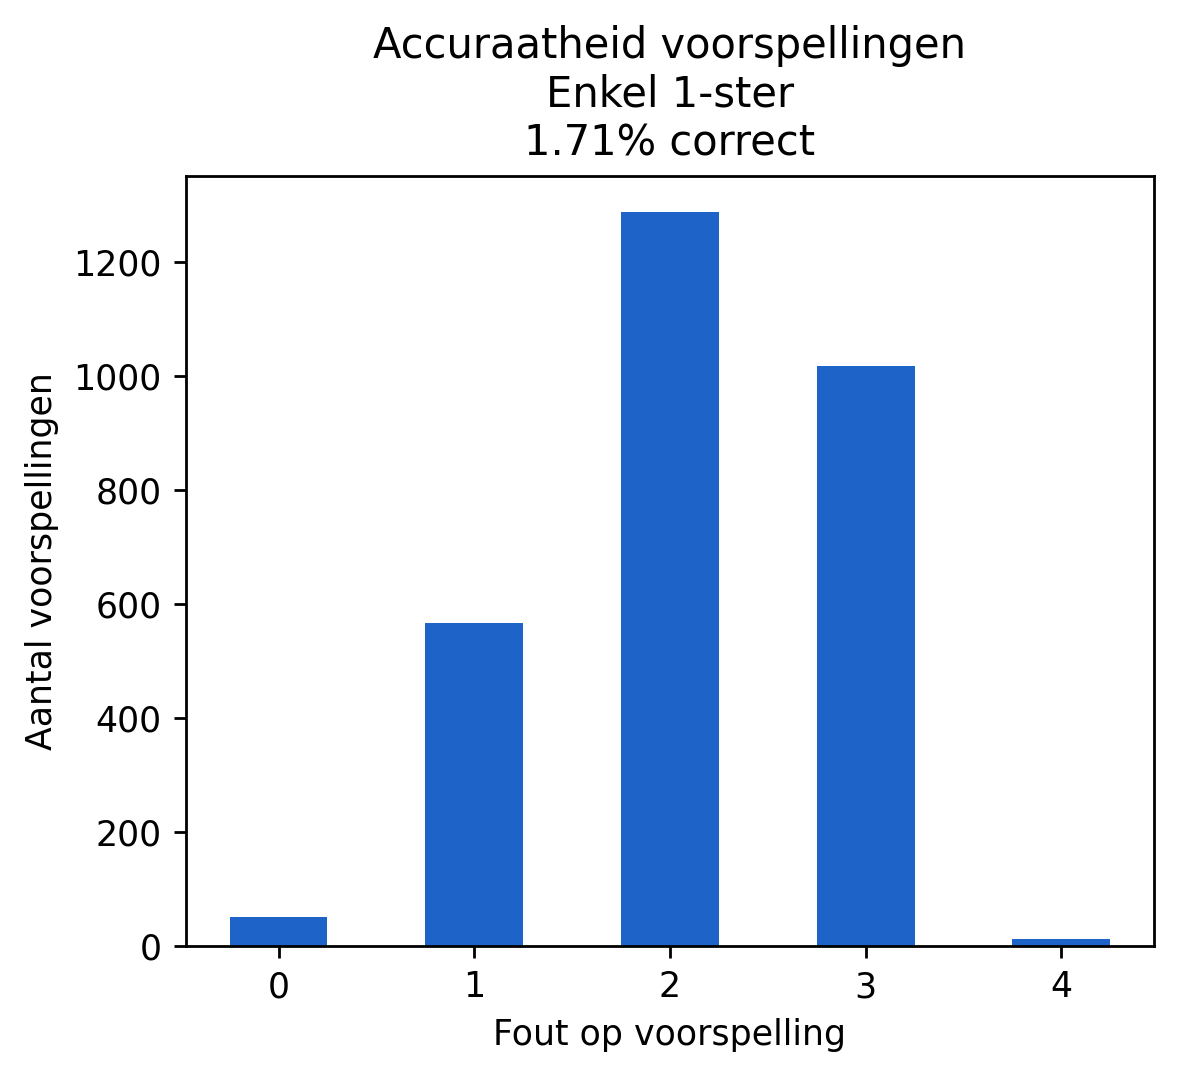
\includegraphics[width=1\linewidth]{fig/chapt5/predictor/extreem_1ster.png}
        \caption{Origineel: MSE}
        \label{fig:chapt5_extreem_4ster_again}
    \end{subfigure}
    \caption{Gemaakte fouten voor alle reviews uit de testset met een specifieke score}
    \label{fig:chapt5_accuracy_lossfunction_combined}
\end{figure}



\section{Vergelijking met andere methoden}
Op dit punt hebben we onderzocht welke NLP-modellen het beste werken om de tekstuele data om te zetten naar vectoren, en weten we welke parametercombinaties de beste performantie opleveren voor het neuraal netwerk. We vergelijken nu onze beste implementatie met andere technieken uit de literatuur, toegepast op dezelfde dataset.

\mijnfiguur[H]{width=15cm}{fig/chapt5/predictor/comparison_implementations.png}{Vergelijken van traditionele methoden en state-of-the-arttechnieken met onze implementatie aan de hand van RMSE. \cite{wide_and_deep_implementation_yelp, narre} Hierbij betekent 'Eigen' dat de inputvector bestaat uit gebruikers- en restaurantprofielen, opgesteld zoals beschreven in deze thesis.}{fig:compare_implementations}

Ons neuraal netwerk is in staat om een lagere loss te scoren dan alle andere geteste technieken op de Yelp Dataset.

Het valt op dat Content-Based Filtering uiterst slecht presteert, waarbij de voorspellingen gemiddeld 3.1 sterren naast de effectieve waarde zitten. Dit komt doordat de labels die gebruikt worden bij CB filtering zeer ijl zijn, en gebruikers veel diverse restaurants bezoeken (\autoref{fig:chapt3_stijging_categorieen_per_gebruiker}). Er zijn te veel zeer specifieke categorieën in de dataset, die ervoor zorgen dat de afstand tussen restaurants te groot is. De hoge loss voor CB bevestigt de hypothese uit \autoref{sec:chapt3_labeled_data_attributes_categories}.\newline
Andere traditionele methoden zoals Item-Item Collaborative Filtering (IICF) en User-User Collaborative Filtering (UUCF) presteren significant beter. Hierbij merken we dat UUCF het een stuk beter doet dan IICF. Bij deze dataset is het dus makkelijker om vergelijkbare gebruikers te modelleren dan restaurants. Dit komt overeen met de analyse dat de NLP-restaurantprofielen minder impact hebben dan de NLP-gebruikersprofielen op de performantie van het neuraal netwerk.
De volgende techniek is een bias recommender op basis van de formule gebruikt door LensKit \cite{bias_lenskit}. Deze recommender presteert gelijkaardig aan UUCF, wat opmerkelijk is voor deze vrij eenvoudige techniek.\newline
We hebben ook twee state-of-the-arttechnieken machine learning-algoritmen vergeleken. Wide \& Deep Learning maakt enkel gebruik de gelabelde data. Aan de andere kant gebruikt DeepCoNN enkel de tekstuele data. De inputvectoren die wij gebruiken voor ons neuraal netwerk zijn gebaseerd op zowel gelabelde als tekstuele data. We merken op dat de implementatie van Wide \& Deep learning merkbaar slechter presteert dan UUCF en de bias recommender. Daartegenover heeft DeepCoNN een lagere RMSE dan alle vorige resultaten waardoor het de beste implementatie is die geen gebruik maakt van onze NLP-inputvectoren.

Ten slotte hebben we zelf nog een tweede model geïmplementeerd dat gebruik maakt van onze eigen inputvectoren zoals beschreven in \autoref{sec:chapt4_nn_input}: een Random Forest. Deze presteert net iets beter dan DeepCoNN, ondanks de relatieve simpliciteit van het model. Dit Random Forest maakt dus ook gebruik van zowel gelabelde als tekstuele data. Deze aanpak lijkt een voordeel te hebben op algoritmen die slechts één van de twee gebruiken. We concluderen dus dat het combineren van gelabelde en tekstuele data een meerwaarde is voor de performantie.

Informatie over de implementaties staat in \verb|src/predictor/implementations|.

\chapter{Conclusie}
% TODO: conclusie
\section{Toekomstig werk}
% TODO: toekomstig werk

% ------------ REFERENCES ------------
% Here you have your bibliography created


\addcontentsline{toc}{chapter}{Bibliografie} %show bibliografie in TOC
\nocite{*}
\printbibliography
% Here you insert your appendices
\appendix

\begin{appendices}

% Dit voegt het woord Bijlage toe aan de titel!
\titleformat{\chapter} % command
  [display] % shape
  {\fontsize{18}{22} \selectfont \coltitle } % format
  {\MakeUppercase{\chaptertitlename \ \thechapter}} % the label
  {-2ex} %separator space
  {\fontsize{24}{32} \selectfont \bf \raggedright \MakeUppercase{\uline{#1}}} %before code
  { } %aft%after code


\chapter[Model development coding]%
{Model development coding}

\section{Pseudocode of the presented algorithm}

\begin{algorithm}[H]
 \SetAlgoLined
 \KwData{this text}
 \KwResult{how to write algorithm with \LaTeX2e }
 initialization\;
 \While{not at end of this document}{
  read current\;
  \eIf{understand}{
   go to next section\;
   current section becomes this one\;
   }{
   go back to the beginning of current section\;
  }
 }
 \caption{How to write algorithms}
\end{algorithm}

\section{Sensitivity base class code \label{senscode}}

\begin{lstlisting}
import os
import numpy as np

from parameter import *
import matplotlib.pyplot as plt
from matplotlib.ticker import FixedLocator, MaxNLocator

class SensitivityAnalysis(object):
    """
    Base class for the Sensitivity Analysis
       
    Parameters
    ----------
    ParsIn : list
        ModPar class instances in list or list of (min,max,'name')-tuples
    
    Attributes
    -----------
    ParsIn : list
        a list of (min,max,'name') values, 
        [(min,max,'name'),(min,max,'name'),...(min,max,'name')]
    parmap : dict
        tracks the sequence of the parameters 
    Pars : list of ModPar instances
        Used when working with the pyFUSE package
    ndim :  int
        number of uncertain input factors
    namelist : list
        list of the uncertain input factors used
    
    """
    
    def __init__(self,ParsIn):
        '''
        Check if all uniform distribution => TODO ! if all -> sobol sampling
        is possible, else, only uniform and normal distribution are supported
        for using the sobol sampling... Here is still work to do!!
        '''
        
        if  isinstance(ParsIn, dict): #bridge with pyFUSE!
            dictlist = []
            for key, value in ParsIn.iteritems():
                dictlist.append(value)
            ParsIn = dictlist
            print ParsIn
       
        #control for other 
        self.ParsIn = ParsIn  
        self.parmap={} #dictionary linking ID and name, since dict instance has no intrinsic sequence
        for i in range(len(ParsIn)):
            if isinstance(ParsIn[i], ModPar): #or isinstance(ParsIn[i], pyFUSE.parameter.ModPar):
                cname = ParsIn[i].name
                self.Pars = ParsIn
                self.ParsIn[i] = (ParsIn[i].min, ParsIn[i].max, cname)
                self.parmap[i] = cname
                
            elif isinstance(ParsIn[i],tuple):
                if ParsIn[i][0] > ParsIn[i][1]:
                    raise Exception('Min value larger than max value')
                if not isinstance(ParsIn[i][0],float) and isinstance(ParsIn[i][1],float):
                    raise Exception('Min and Max value need to be float')
                if not isinstance(ParsIn[i][2],str):
                    raise Exception('Name of par needs to be string')                    
                self.parmap[i] = ParsIn[i][2]
                #create modpar instance of the tuple
                self.Pars=[]
                for par in ParsIn:
                    self.Pars.append(ModPar(par[2],par[0],par[1],(par[0]+par[1])/2.,'randomUniform'))
            else:
                raise Exception('The input type for sampling not correct,\
                choose ModPar instance or list of (min,max)-tuples')        
        
        self.ndim=len(ParsIn)

        self.namelist = [] 
        for i in range(self.ndim):
            self.namelist.append(self.parmap[i])        

    def WritePre(self,filename = 'inputparameterfile', *args, **kwargs):
        '''
        Parameterinputfile for external model, parameters in the columns files
        and every line the input parameters
        
        Parameters
        -----------
        filename : str
            name of the textfile to save
        *args, **kwargs : args
            arguments passed to the numpy savetext-function
        '''
        
        np.savetxt(filename,self.parset2run,*args,**kwargs)
        print 'file saved in directory %s'%os.getcwd()
          
    def ReadRuns(self,filename, *args, **kwargs): 
        '''
        Read model outputs (TODO: do sobol for multiple outputs, iterating the
        post)
        Format is: every output of the ithe MC on ith line
        
        output2evaluate can also be made on a other way

        Parameters
        -----------
        filename : str
            name of the textfile to load    
        *args, **kwargs : args
            arguments passed to the numpy loadtext-function
            
        '''
        self.output2evaluate = np.loadtxt(filename, *args, **kwargs)
\end{lstlisting}




\section{Model input file for PyFUSE model \label{inpufile}}

\begin{lstlisting}[frame=single,columns=fixed]
######################################################
##    Model Parameter input file
##    The parameter is defined by his distribution,
##    boundaries and extra info needed by distribution 
##    provide on each line one parameter with 
##    following information:
##    name : string
##        Name of the parameter
##    minval : float
##        Minimum value of the parameter distribution
##    maxval :  float
##        Maximum value of the parameter distribution
##    optguess : float
##        Optimal guess of the parameter, must be 
##        between min and max value
##    pardistribution : string
##        choose a distributionfrom: randomUniform,
##        randomTriangular, randomTrapezoidal, 
##        randomNormal, randomLogNormal
##    *kargs  :
##        Extra arguments necessary for the 
##        chosen distribution
##	Lines with ## marks are neglected
######################################################
## NAME	MIN MAX OPTGUESS DISTRIBUTION ARGS*
S1max	50. 5000.000 400. randomTriangular 1000.
S2max	100. 10000.000 1000. randomNormal 500. 25. 
fitens 0.01 1.0 0.99 randomLogNormal	0.5 0.2
firchr 0.050 0.950 0.5 randomTrapezoidal 0.4 0.6
fibase 0.050 0.950 0.5 randomUniform
r1 0.050 0.950 0.5 randomUniform
ku 0.01 1000. 0.044 randomUniform
c 0.99 20.0 1. randomUniform
alfa 1.000 250. 150. randomUniform
psi 1.000 5.0 2.5 randomUniform
kappa 0.050 0.950 0.5 randomUniform
ki 0.001 1000. 0.00833 randomUniform
ks 0.001 10000. 0.5 randomUniform
n 1.000 10. 3. randomUniform
v 0.00001 0.250 0.004	randomUniform
vA 0.001 0.250	0.0015 randomUniform
vB 0.001 0.250 0.0015 randomUniform
Acmax 0.050 0.950 0.5 randomUniform
b 0.001 3.0 0.2 randomUniform
loglambda	5.000 10.0 7.5 randomUniform
chi 2.000 5.0 3.5 randomUniform
mut 0.010 5.0 0.6 randomUniform
be 0.99 4. 3.1 randomUniform
alfah	0.01 0.99 0.5 randomUniform
tg 0.0 0.7 0.3 randomUniform
tif 0.0 0.7 0.26 randomUniform
tof 0.0 0.7 0.12 randomUniform
ko 0.01 0.99 0.15 randomUniform
timeo 2. 48 24 randomUniform
timei 2. 250. 20 randomUniform
timeb 200. 10000. 2100. randomUniform
\end{lstlisting}

\end{appendices}

\end{document}
